% Options for packages loaded elsewhere
\PassOptionsToPackage{unicode}{hyperref}
\PassOptionsToPackage{hyphens}{url}
\PassOptionsToPackage{dvipsnames,svgnames,x11names}{xcolor}
%
\documentclass[
  letterpaper,
  DIV=11,
  numbers=noendperiod]{scrartcl}

\usepackage{amsmath,amssymb}
\usepackage{lmodern}
\usepackage{iftex}
\ifPDFTeX
  \usepackage[T1]{fontenc}
  \usepackage[utf8]{inputenc}
  \usepackage{textcomp} % provide euro and other symbols
\else % if luatex or xetex
  \usepackage{unicode-math}
  \defaultfontfeatures{Scale=MatchLowercase}
  \defaultfontfeatures[\rmfamily]{Ligatures=TeX,Scale=1}
\fi
% Use upquote if available, for straight quotes in verbatim environments
\IfFileExists{upquote.sty}{\usepackage{upquote}}{}
\IfFileExists{microtype.sty}{% use microtype if available
  \usepackage[]{microtype}
  \UseMicrotypeSet[protrusion]{basicmath} % disable protrusion for tt fonts
}{}
\makeatletter
\@ifundefined{KOMAClassName}{% if non-KOMA class
  \IfFileExists{parskip.sty}{%
    \usepackage{parskip}
  }{% else
    \setlength{\parindent}{0pt}
    \setlength{\parskip}{6pt plus 2pt minus 1pt}}
}{% if KOMA class
  \KOMAoptions{parskip=half}}
\makeatother
\usepackage{xcolor}
\setlength{\emergencystretch}{3em} % prevent overfull lines
\setcounter{secnumdepth}{-\maxdimen} % remove section numbering
% Make \paragraph and \subparagraph free-standing
\ifx\paragraph\undefined\else
  \let\oldparagraph\paragraph
  \renewcommand{\paragraph}[1]{\oldparagraph{#1}\mbox{}}
\fi
\ifx\subparagraph\undefined\else
  \let\oldsubparagraph\subparagraph
  \renewcommand{\subparagraph}[1]{\oldsubparagraph{#1}\mbox{}}
\fi

\usepackage{color}
\usepackage{fancyvrb}
\newcommand{\VerbBar}{|}
\newcommand{\VERB}{\Verb[commandchars=\\\{\}]}
\DefineVerbatimEnvironment{Highlighting}{Verbatim}{commandchars=\\\{\}}
% Add ',fontsize=\small' for more characters per line
\usepackage{framed}
\definecolor{shadecolor}{RGB}{241,243,245}
\newenvironment{Shaded}{\begin{snugshade}}{\end{snugshade}}
\newcommand{\AlertTok}[1]{\textcolor[rgb]{0.68,0.00,0.00}{#1}}
\newcommand{\AnnotationTok}[1]{\textcolor[rgb]{0.37,0.37,0.37}{#1}}
\newcommand{\AttributeTok}[1]{\textcolor[rgb]{0.40,0.45,0.13}{#1}}
\newcommand{\BaseNTok}[1]{\textcolor[rgb]{0.68,0.00,0.00}{#1}}
\newcommand{\BuiltInTok}[1]{\textcolor[rgb]{0.00,0.23,0.31}{#1}}
\newcommand{\CharTok}[1]{\textcolor[rgb]{0.13,0.47,0.30}{#1}}
\newcommand{\CommentTok}[1]{\textcolor[rgb]{0.37,0.37,0.37}{#1}}
\newcommand{\CommentVarTok}[1]{\textcolor[rgb]{0.37,0.37,0.37}{\textit{#1}}}
\newcommand{\ConstantTok}[1]{\textcolor[rgb]{0.56,0.35,0.01}{#1}}
\newcommand{\ControlFlowTok}[1]{\textcolor[rgb]{0.00,0.23,0.31}{#1}}
\newcommand{\DataTypeTok}[1]{\textcolor[rgb]{0.68,0.00,0.00}{#1}}
\newcommand{\DecValTok}[1]{\textcolor[rgb]{0.68,0.00,0.00}{#1}}
\newcommand{\DocumentationTok}[1]{\textcolor[rgb]{0.37,0.37,0.37}{\textit{#1}}}
\newcommand{\ErrorTok}[1]{\textcolor[rgb]{0.68,0.00,0.00}{#1}}
\newcommand{\ExtensionTok}[1]{\textcolor[rgb]{0.00,0.23,0.31}{#1}}
\newcommand{\FloatTok}[1]{\textcolor[rgb]{0.68,0.00,0.00}{#1}}
\newcommand{\FunctionTok}[1]{\textcolor[rgb]{0.28,0.35,0.67}{#1}}
\newcommand{\ImportTok}[1]{\textcolor[rgb]{0.00,0.46,0.62}{#1}}
\newcommand{\InformationTok}[1]{\textcolor[rgb]{0.37,0.37,0.37}{#1}}
\newcommand{\KeywordTok}[1]{\textcolor[rgb]{0.00,0.23,0.31}{#1}}
\newcommand{\NormalTok}[1]{\textcolor[rgb]{0.00,0.23,0.31}{#1}}
\newcommand{\OperatorTok}[1]{\textcolor[rgb]{0.37,0.37,0.37}{#1}}
\newcommand{\OtherTok}[1]{\textcolor[rgb]{0.00,0.23,0.31}{#1}}
\newcommand{\PreprocessorTok}[1]{\textcolor[rgb]{0.68,0.00,0.00}{#1}}
\newcommand{\RegionMarkerTok}[1]{\textcolor[rgb]{0.00,0.23,0.31}{#1}}
\newcommand{\SpecialCharTok}[1]{\textcolor[rgb]{0.37,0.37,0.37}{#1}}
\newcommand{\SpecialStringTok}[1]{\textcolor[rgb]{0.13,0.47,0.30}{#1}}
\newcommand{\StringTok}[1]{\textcolor[rgb]{0.13,0.47,0.30}{#1}}
\newcommand{\VariableTok}[1]{\textcolor[rgb]{0.07,0.07,0.07}{#1}}
\newcommand{\VerbatimStringTok}[1]{\textcolor[rgb]{0.13,0.47,0.30}{#1}}
\newcommand{\WarningTok}[1]{\textcolor[rgb]{0.37,0.37,0.37}{\textit{#1}}}

\providecommand{\tightlist}{%
  \setlength{\itemsep}{0pt}\setlength{\parskip}{0pt}}\usepackage{longtable,booktabs,array}
\usepackage{calc} % for calculating minipage widths
% Correct order of tables after \paragraph or \subparagraph
\usepackage{etoolbox}
\makeatletter
\patchcmd\longtable{\par}{\if@noskipsec\mbox{}\fi\par}{}{}
\makeatother
% Allow footnotes in longtable head/foot
\IfFileExists{footnotehyper.sty}{\usepackage{footnotehyper}}{\usepackage{footnote}}
\makesavenoteenv{longtable}
\usepackage{graphicx}
\makeatletter
\def\maxwidth{\ifdim\Gin@nat@width>\linewidth\linewidth\else\Gin@nat@width\fi}
\def\maxheight{\ifdim\Gin@nat@height>\textheight\textheight\else\Gin@nat@height\fi}
\makeatother
% Scale images if necessary, so that they will not overflow the page
% margins by default, and it is still possible to overwrite the defaults
% using explicit options in \includegraphics[width, height, ...]{}
\setkeys{Gin}{width=\maxwidth,height=\maxheight,keepaspectratio}
% Set default figure placement to htbp
\makeatletter
\def\fps@figure{htbp}
\makeatother

\KOMAoption{captions}{tableheading}
\makeatletter
\makeatother
\makeatletter
\makeatother
\makeatletter
\@ifpackageloaded{caption}{}{\usepackage{caption}}
\AtBeginDocument{%
\ifdefined\contentsname
  \renewcommand*\contentsname{Table of contents}
\else
  \newcommand\contentsname{Table of contents}
\fi
\ifdefined\listfigurename
  \renewcommand*\listfigurename{List of Figures}
\else
  \newcommand\listfigurename{List of Figures}
\fi
\ifdefined\listtablename
  \renewcommand*\listtablename{List of Tables}
\else
  \newcommand\listtablename{List of Tables}
\fi
\ifdefined\figurename
  \renewcommand*\figurename{Figure}
\else
  \newcommand\figurename{Figure}
\fi
\ifdefined\tablename
  \renewcommand*\tablename{Table}
\else
  \newcommand\tablename{Table}
\fi
}
\@ifpackageloaded{float}{}{\usepackage{float}}
\floatstyle{ruled}
\@ifundefined{c@chapter}{\newfloat{codelisting}{h}{lop}}{\newfloat{codelisting}{h}{lop}[chapter]}
\floatname{codelisting}{Listing}
\newcommand*\listoflistings{\listof{codelisting}{List of Listings}}
\makeatother
\makeatletter
\@ifpackageloaded{caption}{}{\usepackage{caption}}
\@ifpackageloaded{subcaption}{}{\usepackage{subcaption}}
\makeatother
\makeatletter
\@ifpackageloaded{tcolorbox}{}{\usepackage[many]{tcolorbox}}
\makeatother
\makeatletter
\@ifundefined{shadecolor}{\definecolor{shadecolor}{rgb}{.97, .97, .97}}
\makeatother
\makeatletter
\makeatother
\ifLuaTeX
  \usepackage{selnolig}  % disable illegal ligatures
\fi
\IfFileExists{bookmark.sty}{\usepackage{bookmark}}{\usepackage{hyperref}}
\IfFileExists{xurl.sty}{\usepackage{xurl}}{} % add URL line breaks if available
\urlstyle{same} % disable monospaced font for URLs
\hypersetup{
  pdftitle={Foundations of HPC - Assignment},
  pdfauthor={Filippo Olivo},
  colorlinks=true,
  linkcolor={blue},
  filecolor={Maroon},
  citecolor={Blue},
  urlcolor={Blue},
  pdfcreator={LaTeX via pandoc}}

\title{Foundations of HPC - Assignment}
\author{Filippo Olivo}
\date{}

\begin{document}
\maketitle
\ifdefined\Shaded\renewenvironment{Shaded}{\begin{tcolorbox}[interior hidden, boxrule=0pt, sharp corners, frame hidden, borderline west={3pt}{0pt}{shadecolor}, enhanced, breakable]}{\end{tcolorbox}}\fi

\renewcommand*\contentsname{Table of contents}
{
\hypersetup{linkcolor=}
\setcounter{tocdepth}{4}
\tableofcontents
}
\newpage

\noindent

\hypertarget{excercise-1}{%
\section{Excercise 1}\label{excercise-1}}

\hypertarget{introduction}{%
\subsection{Introduction}\label{introduction}}

The aim of the excercise is to implement a parallel version of the
Conway's Game of Life through MPI and OpenMP. Game of life is a zero
player game which evolution depends only on the initial conditions. In
this project I have implemented three possible iteration tecniques:

\begin{itemize}
\item
  Static iteration: we freeze the system at each state \(s_i\) and then
  we evaluate the new cell status \(s_{i+1}\) based on the system at
  state \(s_i\)
\item
  Ordered iteration: we start from the cell (0,0) and we evolve by lines
\end{itemize}

\begin{figure}

\begin{minipage}[t]{0.20\linewidth}

{\centering 

~

}

\end{minipage}%
%
\begin{minipage}[t]{0.25\linewidth}

{\centering 

\raisebox{-\height}{

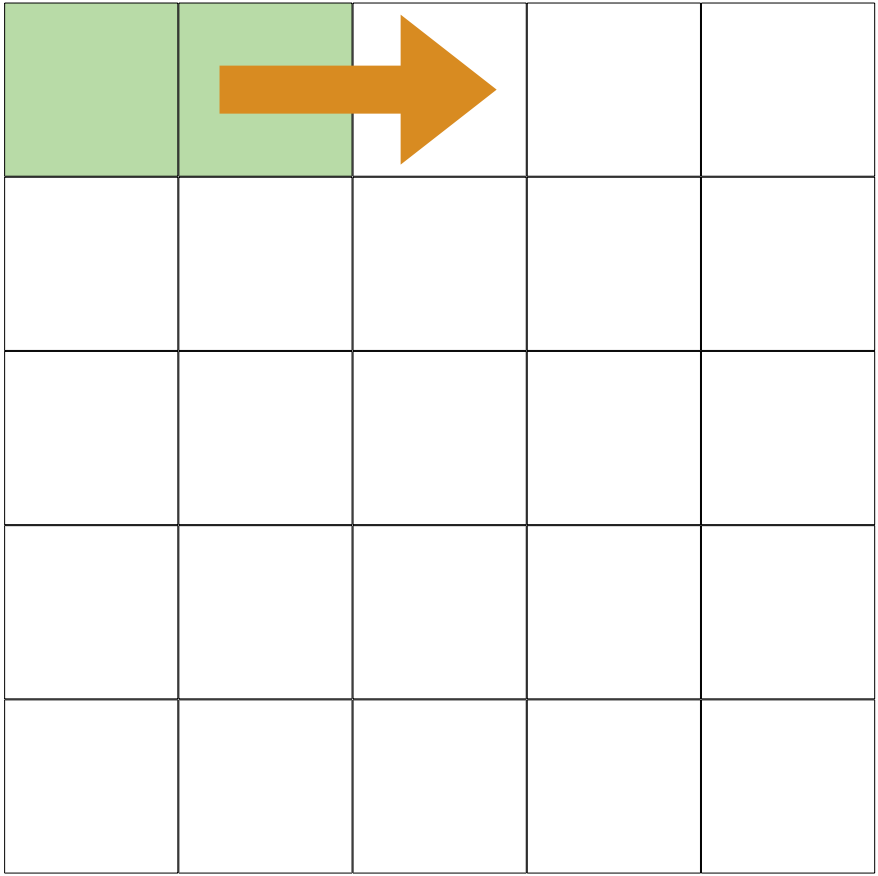
\includegraphics{img/iterate_ordered_intro_1.png}

}

}

\end{minipage}%
%
\begin{minipage}[t]{0.10\linewidth}

{\centering 

~

}

\end{minipage}%
%
\begin{minipage}[t]{0.25\linewidth}

{\centering 

\raisebox{-\height}{

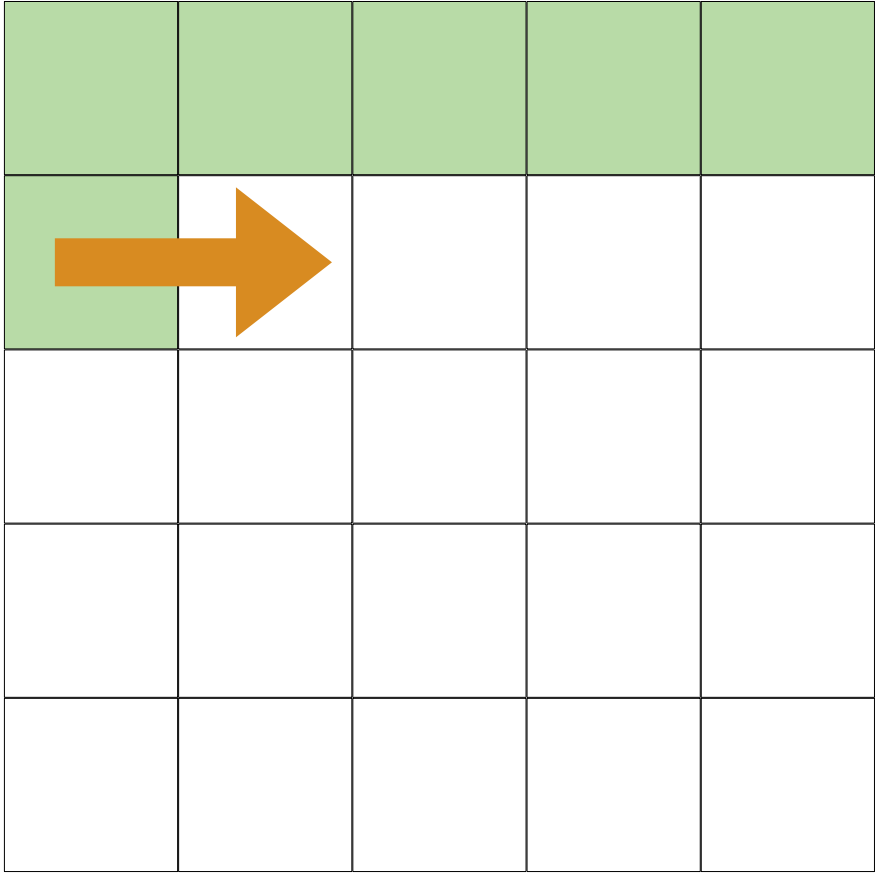
\includegraphics{img/iterate_ordered_intro_2.png}

}

}

\end{minipage}%
%
\begin{minipage}[t]{0.20\linewidth}

{\centering 

~

}

\end{minipage}%

\end{figure}

\begin{itemize}
\tightlist
\item
  Wave iteration: wave that spread in diagonal from cell (0,0) (futher
  details below)
\end{itemize}

\hypertarget{metodology}{%
\subsection{Metodology}\label{metodology}}

The program is written in C language and it can perform the three types
of operations explained in the previous section. The world must be read
from a \texttt{pgm} file and which is converted in arrays of
\texttt{unsigned\ char}. The choice of using a matrix of
\texttt{unsigned\ char} has been made to reduce the usage of RAM. Inside
the program the alive cells are represented with the number 0, while the
dead cells are represented with the number 255, respectively the black
and the white colour in the output grid. The program consist in mainly
four modules:

\begin{enumerate}
\tightlist
\item
  Read and write: a support module that read/write from/to a
  \texttt{pgm} file. In order to distribute the data across the nodes
  the reading operation is done in parallel (if the code is runned on
  more than one MPI Task)
\item
  Run static: implement the static iteration already mentioned above.
\item
  Run ordered: implement the ordered iteration already mentioned above.
  Ordered iterations are by definition serial and, for this reason, I
  have only implemented a domain decomposition across the nodes (see
  below for futher details)
\item
  Run wave: implement the wave iteration already mentioned above. This
  implmenetation is done only with OpenMP (see below for further
  details)
\end{enumerate}

To evaluate the performances I have run multiple test on the Epyc and
Thin nodes of the orfeo cluster changing properly the number of MPI
processes and OpenMP threads. In this section I am mainly interested in
the speed up described by the formula below: \[
    \text{Speed up} = \frac{T_s}{T_{np}}
\] Where \(T_s\) is the time taken by a single process and \(T_{np}\) is
the time taken by n processes (note that the ideal speed up is given by
\(\text{Speed up} = n\) (\(n\) is the number of processes)

\hypertarget{implementation}{%
\subsection{Implementation}\label{implementation}}

In this section I discuss some technical aspects of the code, in
particular I focus on the parallelization methods.

\hypertarget{read-and-write-operations}{%
\subsubsection{Read and write
operations}\label{read-and-write-operations}}

Reading from \texttt{pgm} files operation is performed in parallel: from
a single \texttt{pgm} file the master thread reads the header, captures
the parameter, such as the size of the matrix, the max value, and the
type of the file, and broadcasts them to other MPI Tasks. Each process
reads and stores inside an array of \texttt{unsigned\ char} a matrix of
size equal to \(size_{world}\)x\(R_i\) where \(R_i\) is the number of
rows, calculated by the formula:

\[
R_i = 
\begin{cases}
\text{floor}\bigg(\frac{size_{world}}{n_{MPI \; Process}}\bigg)+1 & \text{if module}(size_{world},n_{MPI \; Process}) > 0 \\
\text{floor}\bigg(\frac{size_{world}}{n_{MPI \; Process}}\bigg) & \text{otherwise} \\
\end{cases}
\]

The reading is performed through MPI I/O and more precisely by calling
the function \texttt{MPI\_File\_read}

Writing is performed in parallel: each MPI Task writes its output in a
separate file and a bash script perform the joining of the files.

\hypertarget{initialization}{%
\subsubsection{Initialization}\label{initialization}}

The initialization part is performed in parallel. The work is subdivided
among the MPI Tasks and more precisely each of those has to initialize a
submatrix of size \(size_{world}\cdot R_i\), where \(R_i\) is a positive
number given by the formula: \[
R_i = 
\begin{cases}
\text{floor}\bigg(\frac{size_{world}}{n_{MPI \; Process}}\bigg)+1 & \text{if module}(size_{world},n_{MPI \; Process}) > 0 \\
\text{floor}\bigg(\frac{size_{world}}{n_{MPI \; Process}}\bigg) & \text{otherwise} \\
\end{cases}
\]

A for loop, parallelized through the usage of OpenMP, perform the
initialization of the submatrix. The scheduling used for the loop
paralleliization is static due to the balanced workload that each thread
has to perform at each iteration. Increasing/decreasing the chunk size
does not improve the overall performances and, for this reason, I have
decided to keep it to the default value (chunk size =
num\_it/num\_threads). After the initialization, the OpenMP parallel
region ends. Each MPI Tasks, in the correct order, writes on the target
file its submtrix (the process 0 write also the initial lines that
specify the type of file and the dimension of the image).

\hypertarget{static-iteration-method}{%
\subsubsection{Static iteration method}\label{static-iteration-method}}

The apporch used to parallelize this type of operation is the domain
decomposition: each MPI Task has to work on a submatrix of size
\(size_{world}\times R_i\) as defined in the previous subsection. In
order to allow each MPI Task to calculate the new status of its cells,
the MPI Task needs to have also the last line of the submatrix of the
process before (rank-1 or size-1 for the first process) and the first
line of the submatrix of the process after (rank+1 or 0 for the process
size-1). Below is shown an example with a matrix 6x6 and 3 MPI Processes
(in this case this process has a submatrix of size 2x3 and 3 additional
rows).

\begin{figure}

{\centering 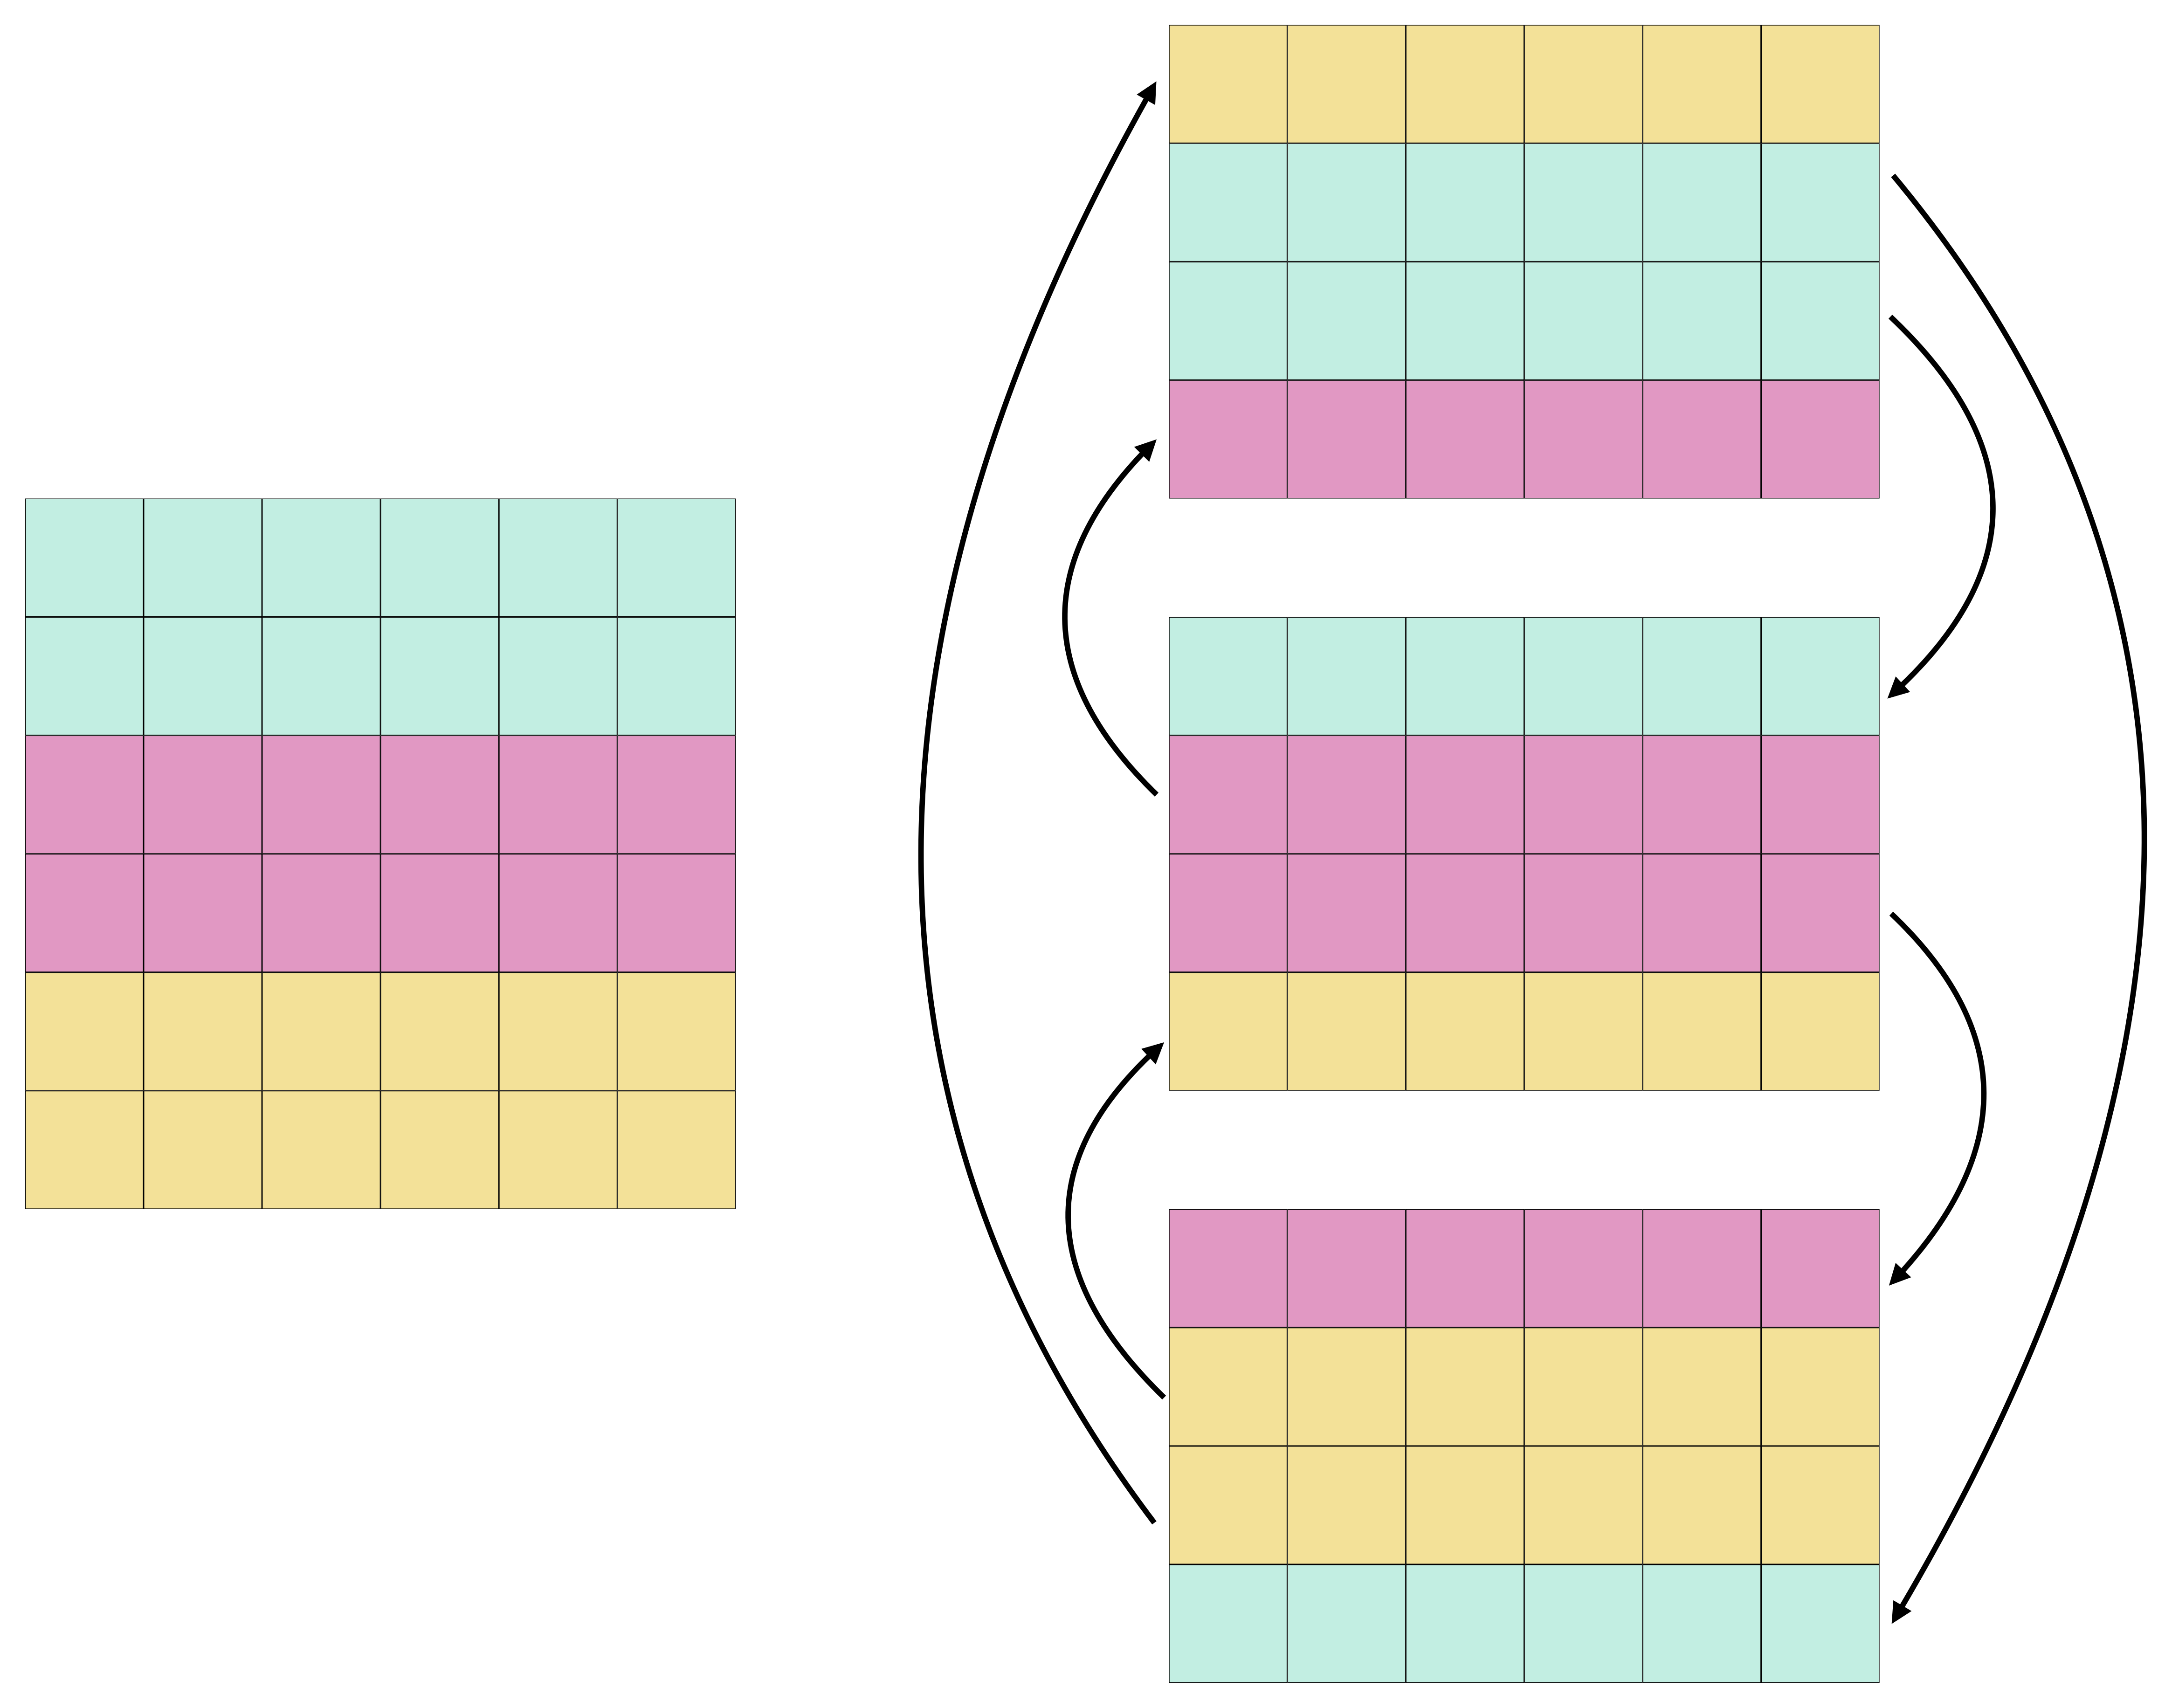
\includegraphics[width=\textwidth,height=2.08333in]{img/domain_decomposition_static.png}

}

\caption{Domain decomposition}

\end{figure}

Each process create another matrix of the same size of the previous one.
The idea is to calculate the status \(s_{i+1}\) from the matrix of the
status \(s_{i}\). At the beggining of each iteration each MPI Process:

\begin{itemize}
\tightlist
\item
  Send (through a non-blocking send) its first and last rows
\item
  Received from/to the other processes the necessary rows
\item
  Store them in the local matrix that contains the values of the
  iteration \(s_i\)
\end{itemize}

In order to avoid errors each at iteration the tag changes. It could
happen that a MPI Task is one complete iteration in advance than the
following or previous MPI Tasks. Find above the lines that perform the
send and receive of the rows:

\begin{figure}

{\centering 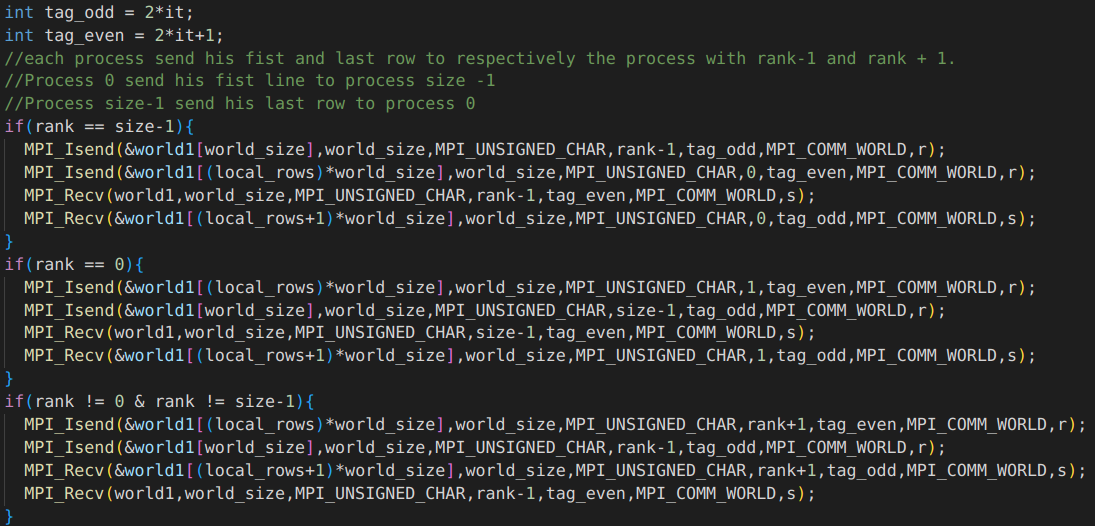
\includegraphics[width=\textwidth,height=2.5in]{img/send_receive_ordered.png}

}

\caption{Send and receive process}

\end{figure}

Then the update method is called it consists in a for loop which, for
each cell of status \(s_{i+1}\):

\begin{itemize}
\tightlist
\item
  read the value of all the neighbour from matrix of status \(s_{i}\)
\item
  calculate the value of the new status and write it on the new matrix
\end{itemize}

This for loop is parallelized with OpenMP: each MPI Task has to update a
bunch of cells independently from other OpenMP threads. The best
scheduling policy is the static one and this is reasonable due to the
almost costant workload of the iterations. As it concern the chunk size,
an increase/decrease of it does not bring a significant improvement of
the overall performances of the program. For this reason, I have decided
to keep it at the default value (chunk size = num\_it/num\_threads).
Note that the program keeps in memory only the matrix of the actual and
the previous status.

\hypertarget{ordered-iteration-method}{%
\subsubsection{Ordered iteration
method}\label{ordered-iteration-method}}

Similar to the static iteration method, the ordered iteration method
uses a domain decomposition approch. As in the previous case each
process reads a portion of the world. Before starting the iteration
process, the last MPI Task sends respectively its last row to process 0
and each process sends his first row to the previous process. Each
process, at the end of the elaboration, sends its last row to the
previous process. Note that in this case an MPI task start the
computation when it receives the last row of the following process.

In this way I expect that the parallelization does not improve the
computational time but we have to consider that with this type domain
decomposition the memory scales. Because of the fact that each MPI Task
has its submatrix directly read from the file the overall size of the
matrix can be larger then the RAM of a single node. In the serial
problem the entire world must fit inside the RAM of a single node.

\hypertarget{wave-iteration-method}{%
\subsubsection{Wave iteration method}\label{wave-iteration-method}}

The data structure that are needed for this method are two matrices of
size \(size_{world} \times size_{world}\) and an array of struct Cell
(below the definition).

\begin{Shaded}
\begin{Highlighting}[]
\KeywordTok{struct}\NormalTok{ Cell}\OperatorTok{\{}
  \DataTypeTok{long}\NormalTok{ row}\OperatorTok{;}
  \DataTypeTok{long}\NormalTok{ col}\OperatorTok{;}
\OperatorTok{\};}
\end{Highlighting}
\end{Shaded}

A single iteration starts with the update of the cell (0,0) of the
world. After the update, a struct Cell variable is created for all the
neightbour of the cell (0,0) and stored in an array. The only purpose of
the struct is to represent in a more simple way the cells that must be
updated in the next step of the iteration.

Before starting the next step of the single iteration, also the matrix
that represent the previous status of the world is updated with the new
values. On the following step each OpenMP thread updates a bunch of
Cells presents in the array using the previous state world (\texttt{for}
loops parallelized through OpenMP). This procedure continues until the
last row and column are updated.

\begin{figure}

{\centering 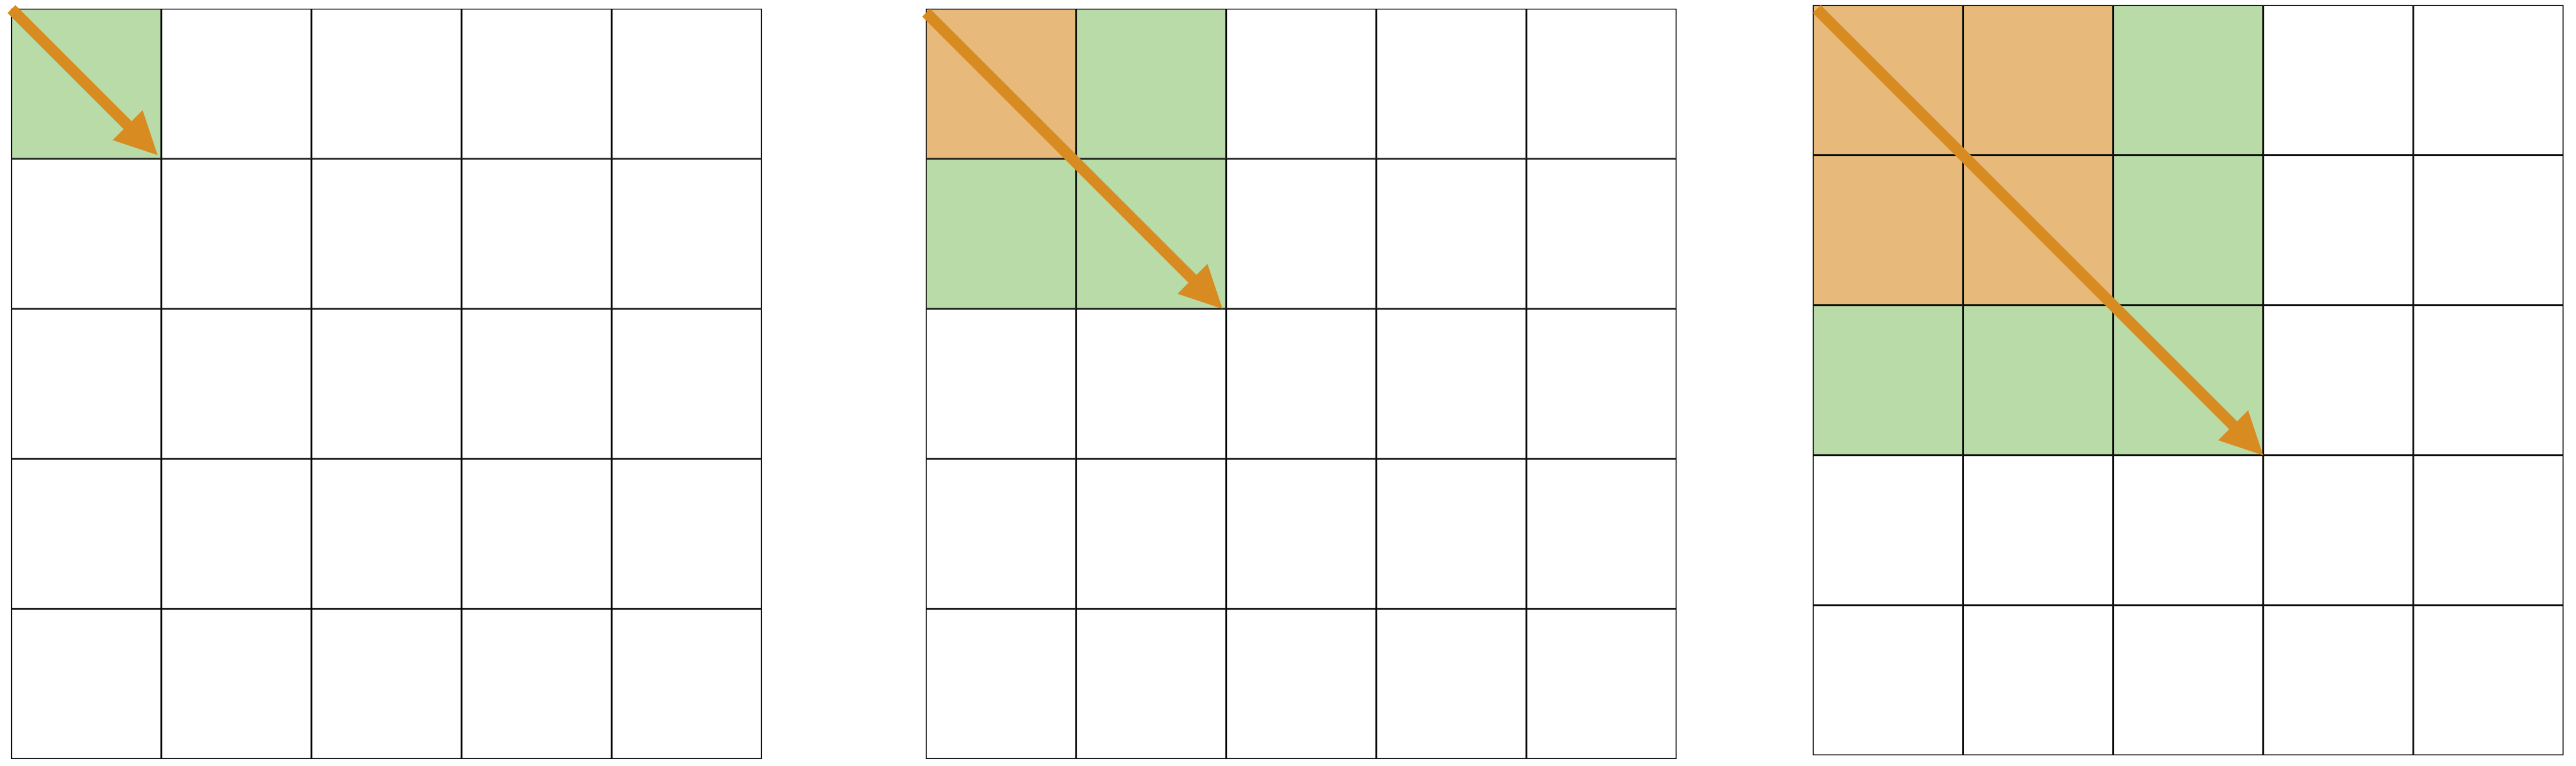
\includegraphics[width=\textwidth,height=2.08333in]{img/wave_update.png}

}

\caption{Wave iteration}

\end{figure}

The best schedule of the for loop is static, as expected, due to the
balanced workload of each iteration of the for loop. I have chosen to
use chunk size equal to 1 in order to parallelize the the update
procudure starting from the second step of each iteration.

\hypertarget{code-validation}{%
\subsection{Code validation}\label{code-validation}}

To asses that the code works properly I have started considering a very
small problem with size \(10 \times 10\) and the serial version of the
program. First I have updated the initial world with only one time and
assess that the result was correct. After having assessed that the
serial program works properly for a single iteration I have tried to do
two iterations and also in this case I manually verified the output.
Below the used example:

\begin{figure}

{\centering 
\includegraphics[width=\textwidth,height=2.08333in]{img/test_static.png}

}

\caption{Test run static}

\end{figure}

After this procedure I have assesed that the serial cose works properly.
To test the parallel computation I have calculated the sha256 for the
serial and the parallel output (for different number of MPI tasks,
OpenMP threads and size of the world) and verified that these two values
were equal.

\hypertarget{result-and-performances}{%
\subsection{Result and performances}\label{result-and-performances}}

I have performed several test to evaluate the computation time and the
speedup of the different type of evolution, with different size and with
different OpenMP and MPI options. The time has been taken from the start
to the end of the MPI parallel region, which almost coincide with the
overall time of the program.

\hypertarget{iterate-static}{%
\subsubsection{Iterate static}\label{iterate-static}}

The measure made for this type of iteration method are:

\begin{itemize}
\tightlist
\item
  \textbf{OpenMP Scalability}
\item
  \textbf{MPI Strong Scalability}
\item
  \textbf{Weak MPI Scalability}
\end{itemize}

All the measurements in this section have been made on the Epyc and Thin
node of the High performance computing cluster Orfeo whithout the SMT.

\hypertarget{openmp-scalability}{%
\paragraph{OpenMP Scalability}\label{openmp-scalability}}

We want to measure how much the program scales when we increase the
number of OpenMP threads. The test has been made with the OpenMP option
\texttt{OMP\_PROC\_BIND=close} and I have placed one single MPI Task for
each socket with the option \texttt{-\/-map-by\ socket} when I have used
1 or 2 sockets on the same machine and with the options
\texttt{-\/-map-by\ node\ -\/-bind-to\ socket} when I have used more
than 3 socket (up to 6 socket for Epyc nodes and up to 4 for Thin node).
For the Epyc node I have tested two different sizes of the matrix with
different number of iterations:

\begin{itemize}
\tightlist
\item
  Size: \(25000\times 25000\) and 50 iterations
\item
  Size: \(25000\times 25000\) and 100 iterations
\item
  Size \(12500\times 125000\) and 50 iterations
\end{itemize}

The graphs below show the OpenMP scalability for the epyc nodes:

\begin{figure}

{\centering 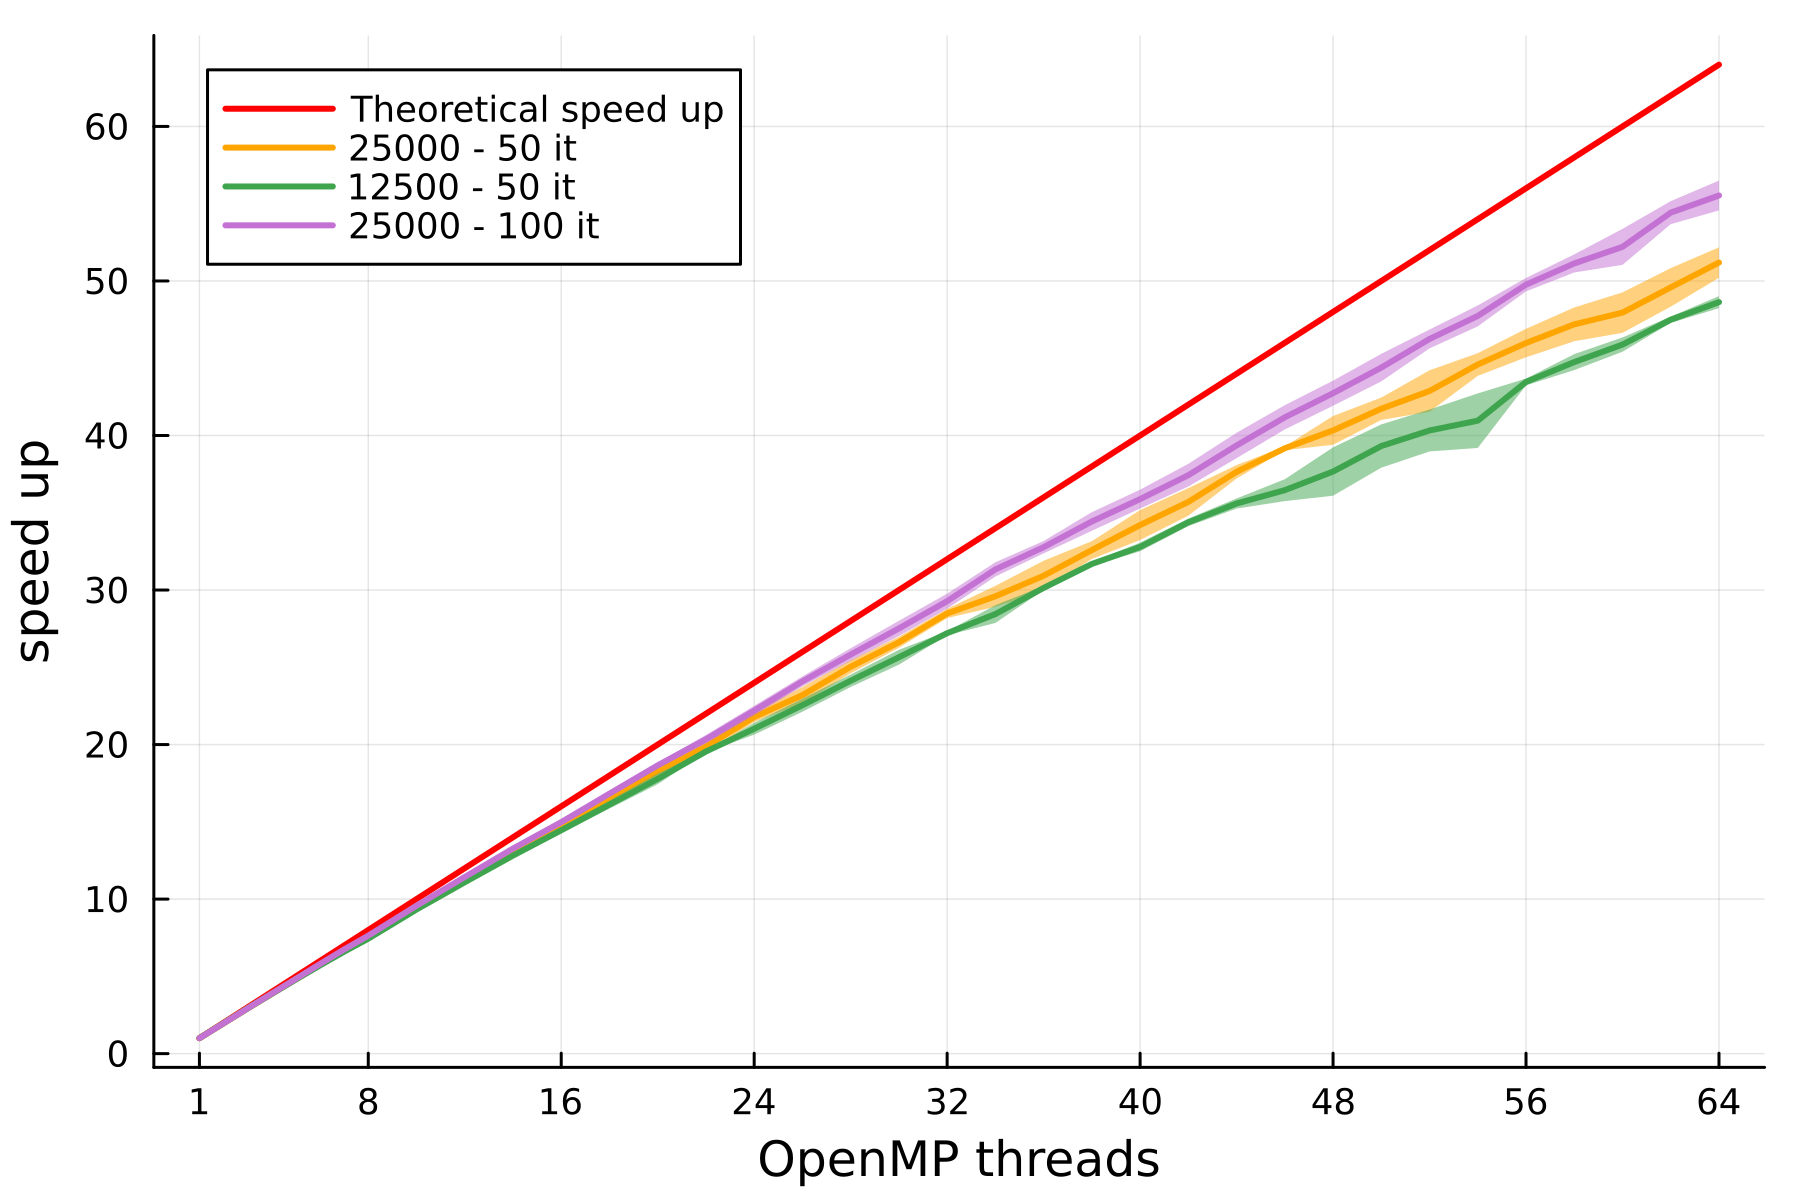
\includegraphics[width=\textwidth,height=3.64583in]{img/epyc_1_socket.png}

}

\caption{OpenMP scalability - 1 socket}

\end{figure}

\begin{figure}

{\centering 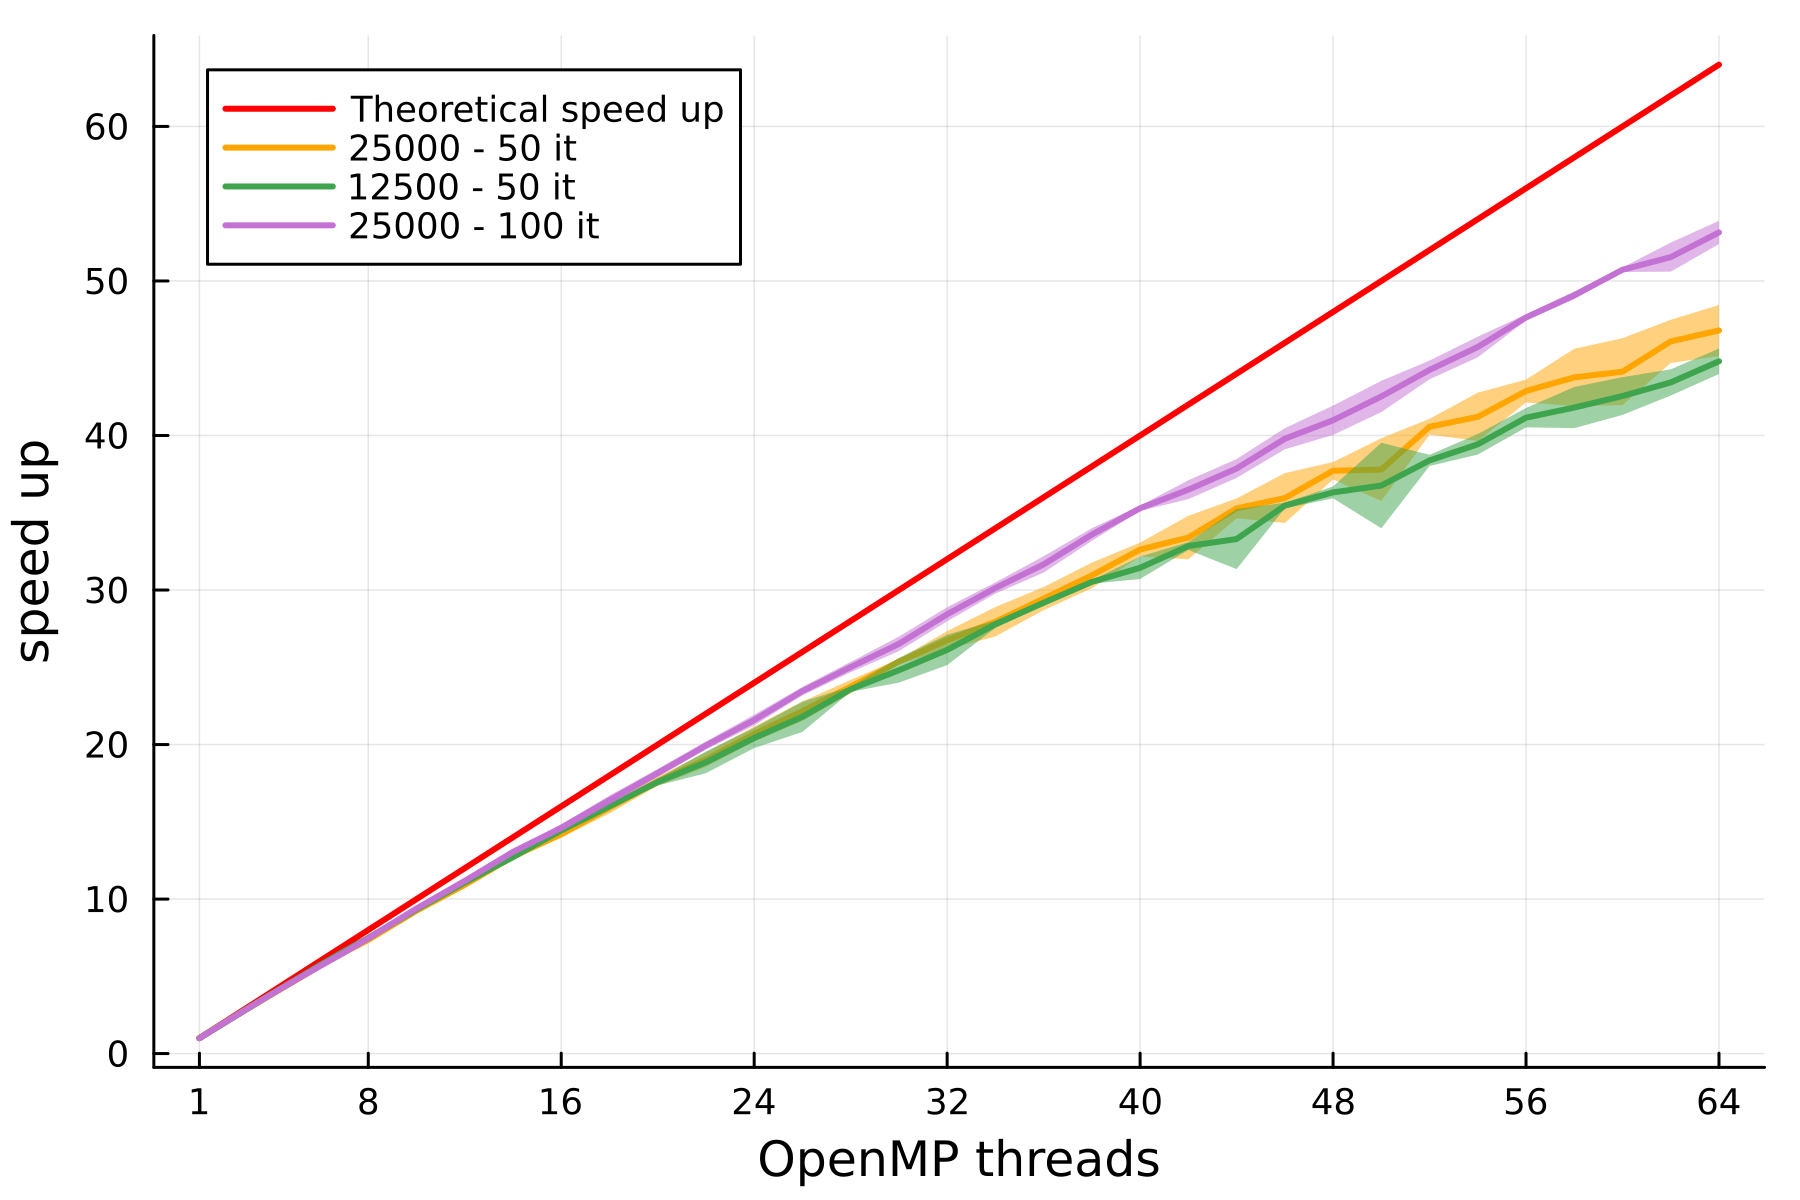
\includegraphics[width=\textwidth,height=3.64583in]{img/epyc_2_sockets.png}

}

\caption{OpenMP scalability - 2 sockets}

\end{figure}

\begin{figure}

{\centering 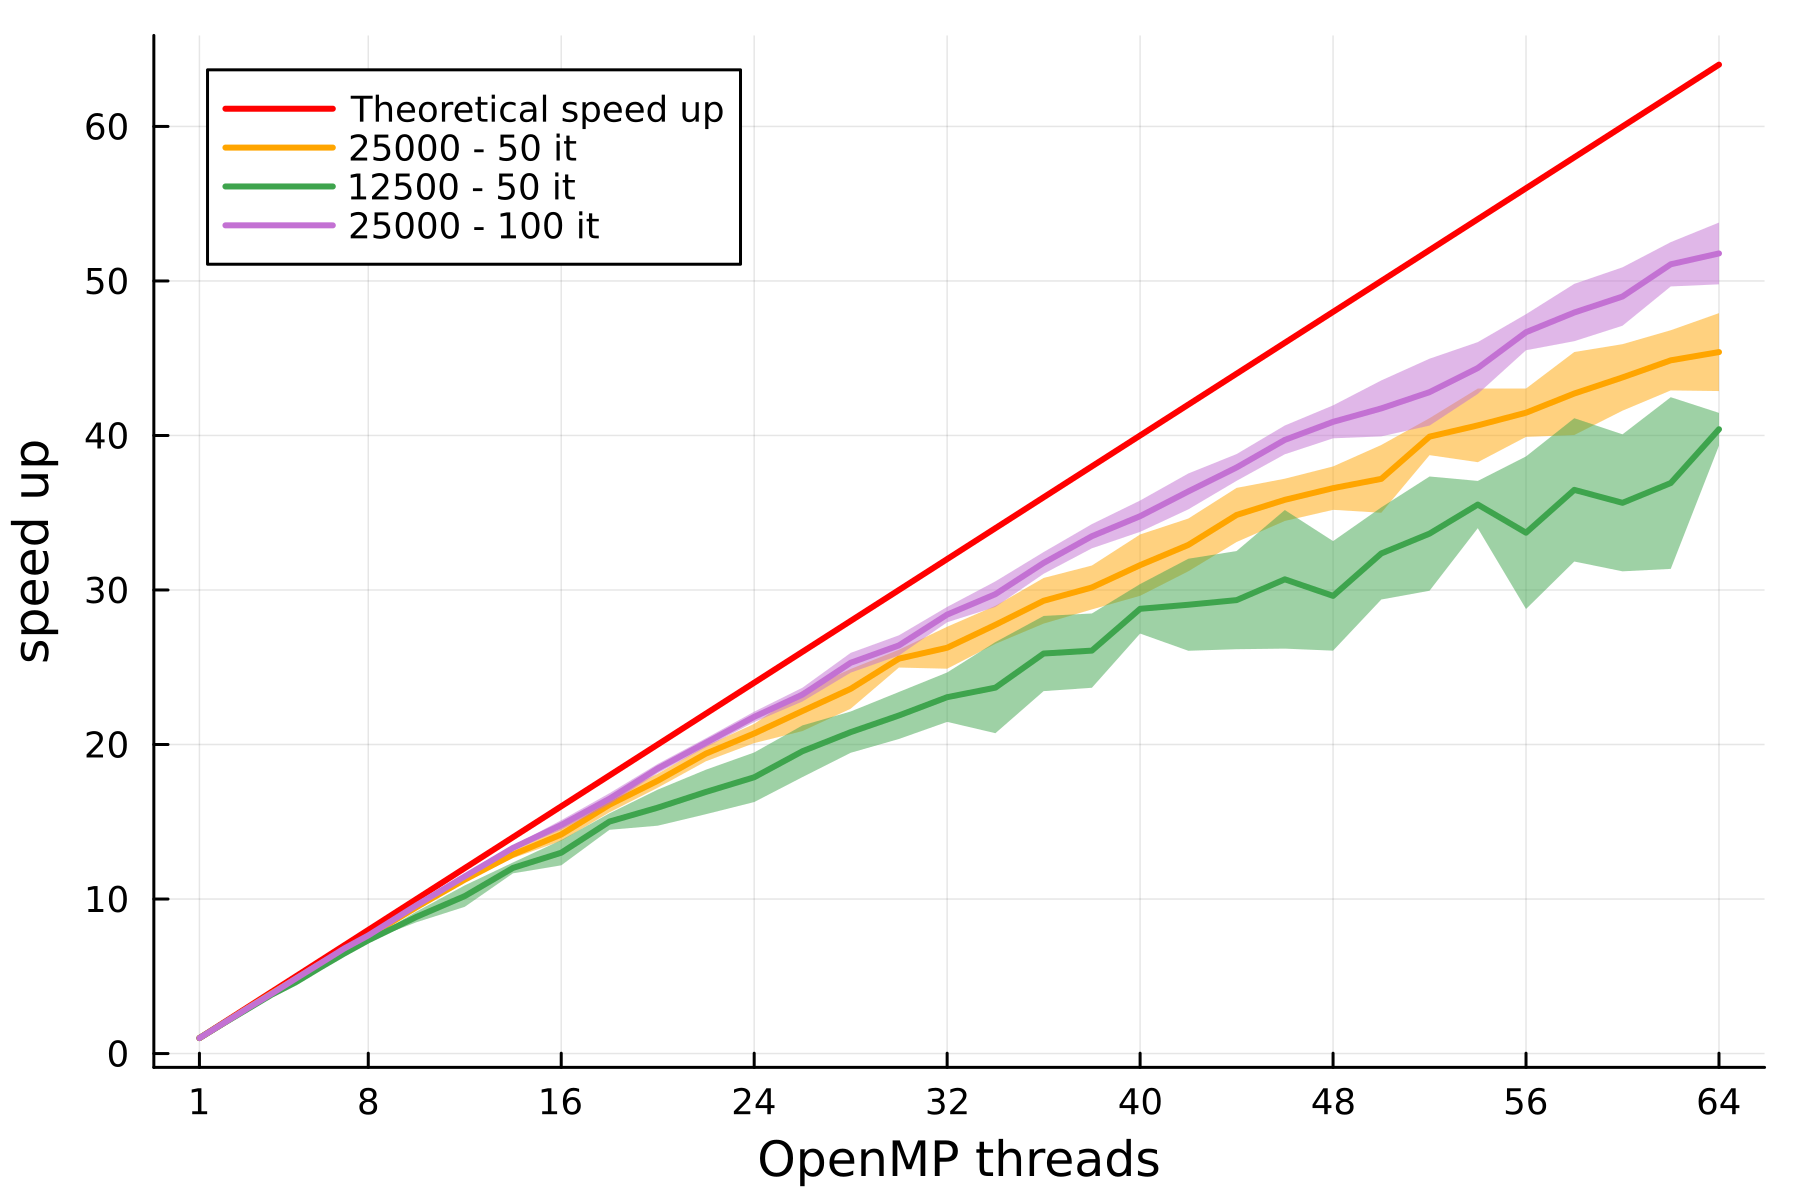
\includegraphics[width=\textwidth,height=3.64583in]{img/epyc_3_sockets.png}

}

\caption{OpenMP scalability - 3 sockets}

\end{figure}

\begin{figure}

{\centering 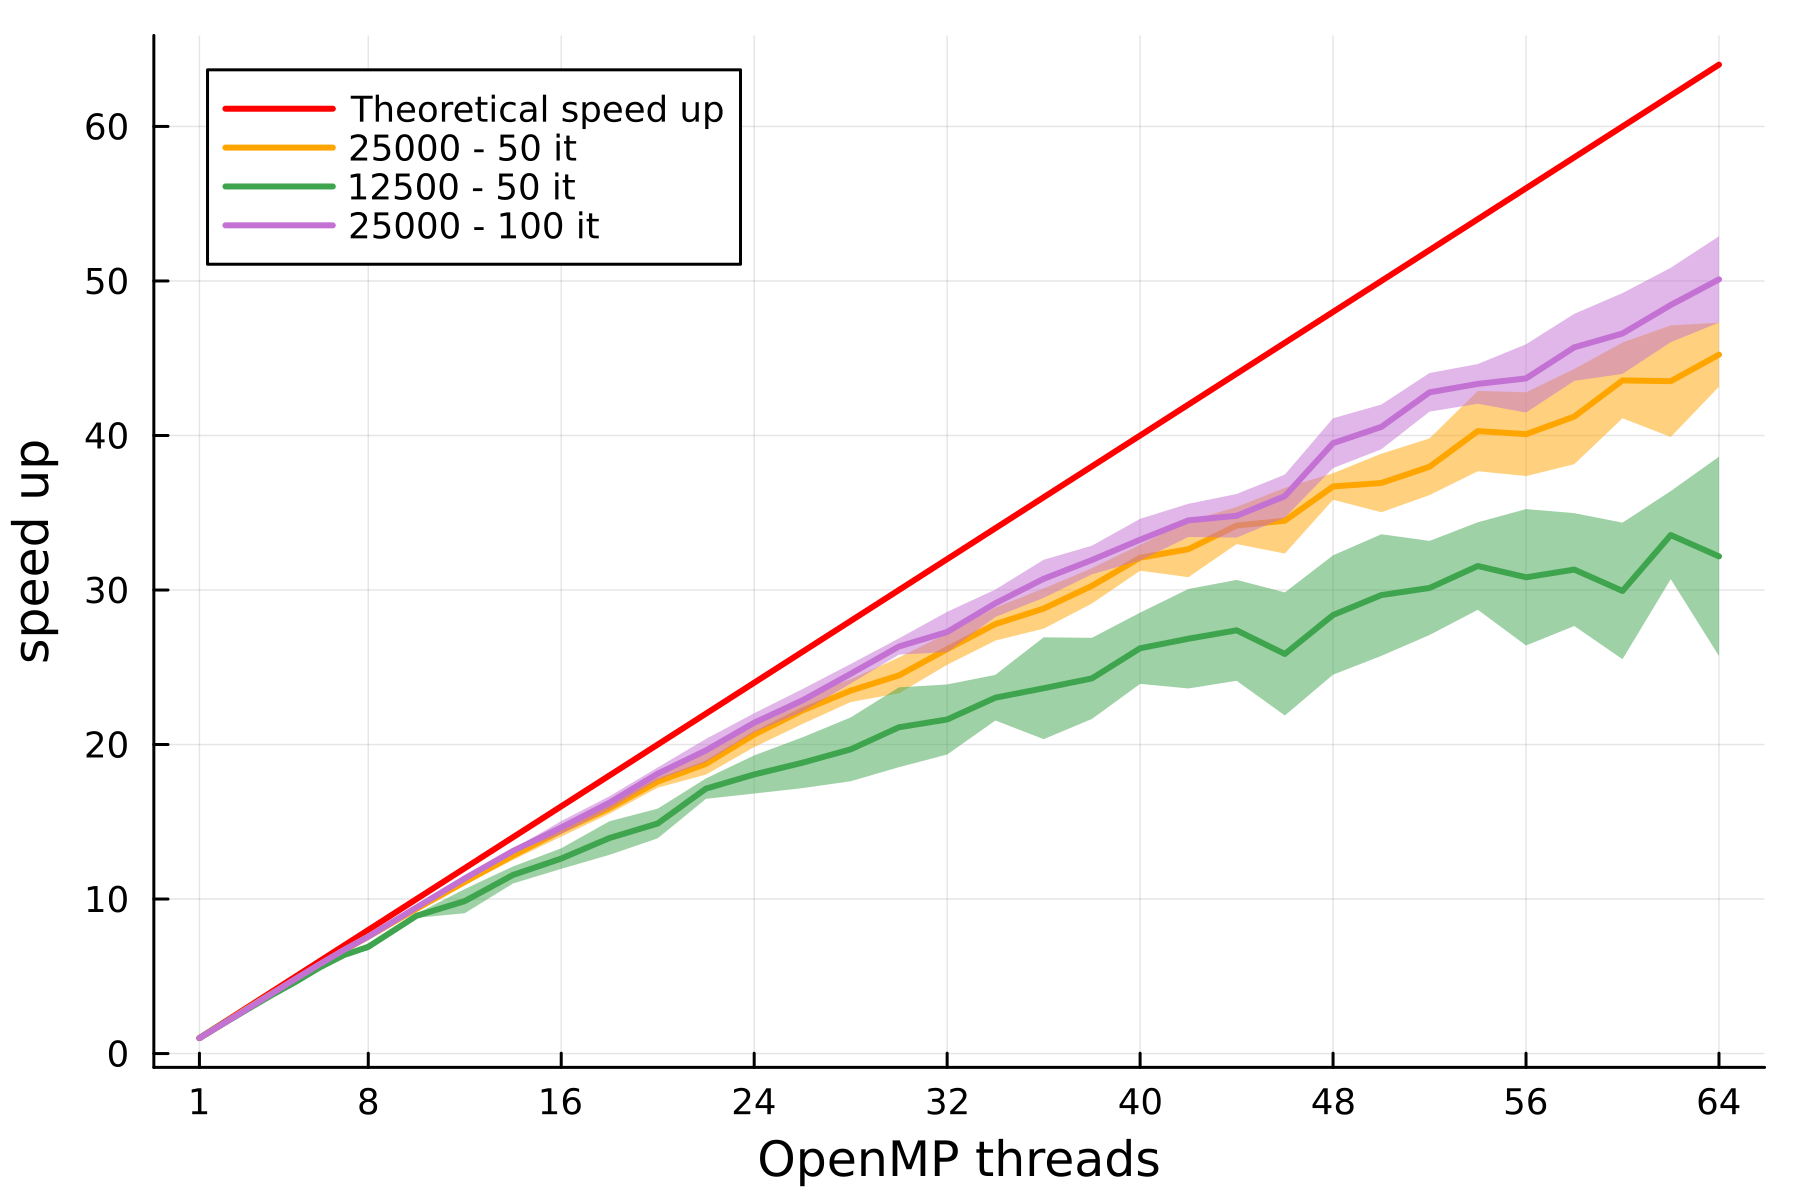
\includegraphics[width=\textwidth,height=3.64583in]{img/epyc_4_sockets.png}

}

\caption{OpenMP scalability - 4 sockets}

\end{figure}

\begin{figure}

{\centering 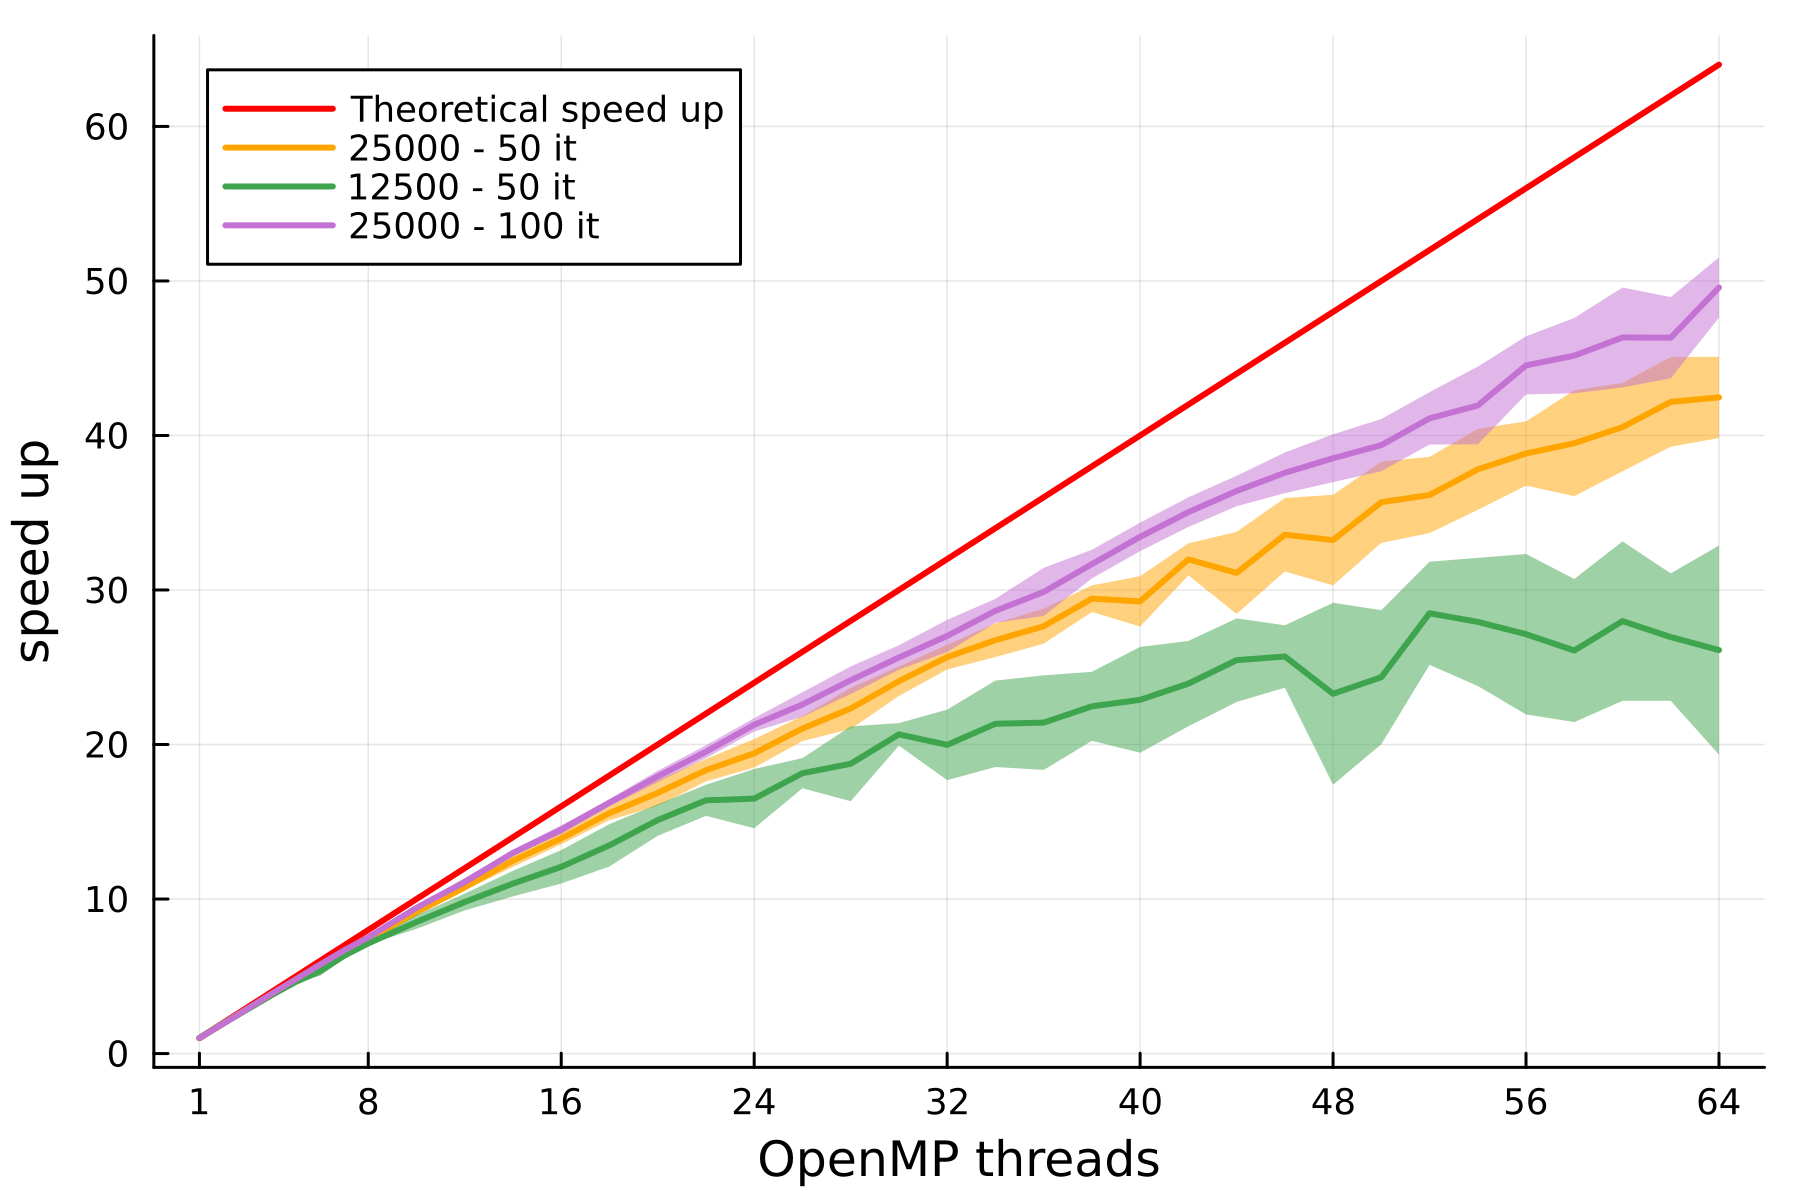
\includegraphics[width=\textwidth,height=3.64583in]{img/epyc_5_sockets.png}

}

\caption{OpenMP scalability - 5 sockets}

\end{figure}

\begin{figure}

{\centering 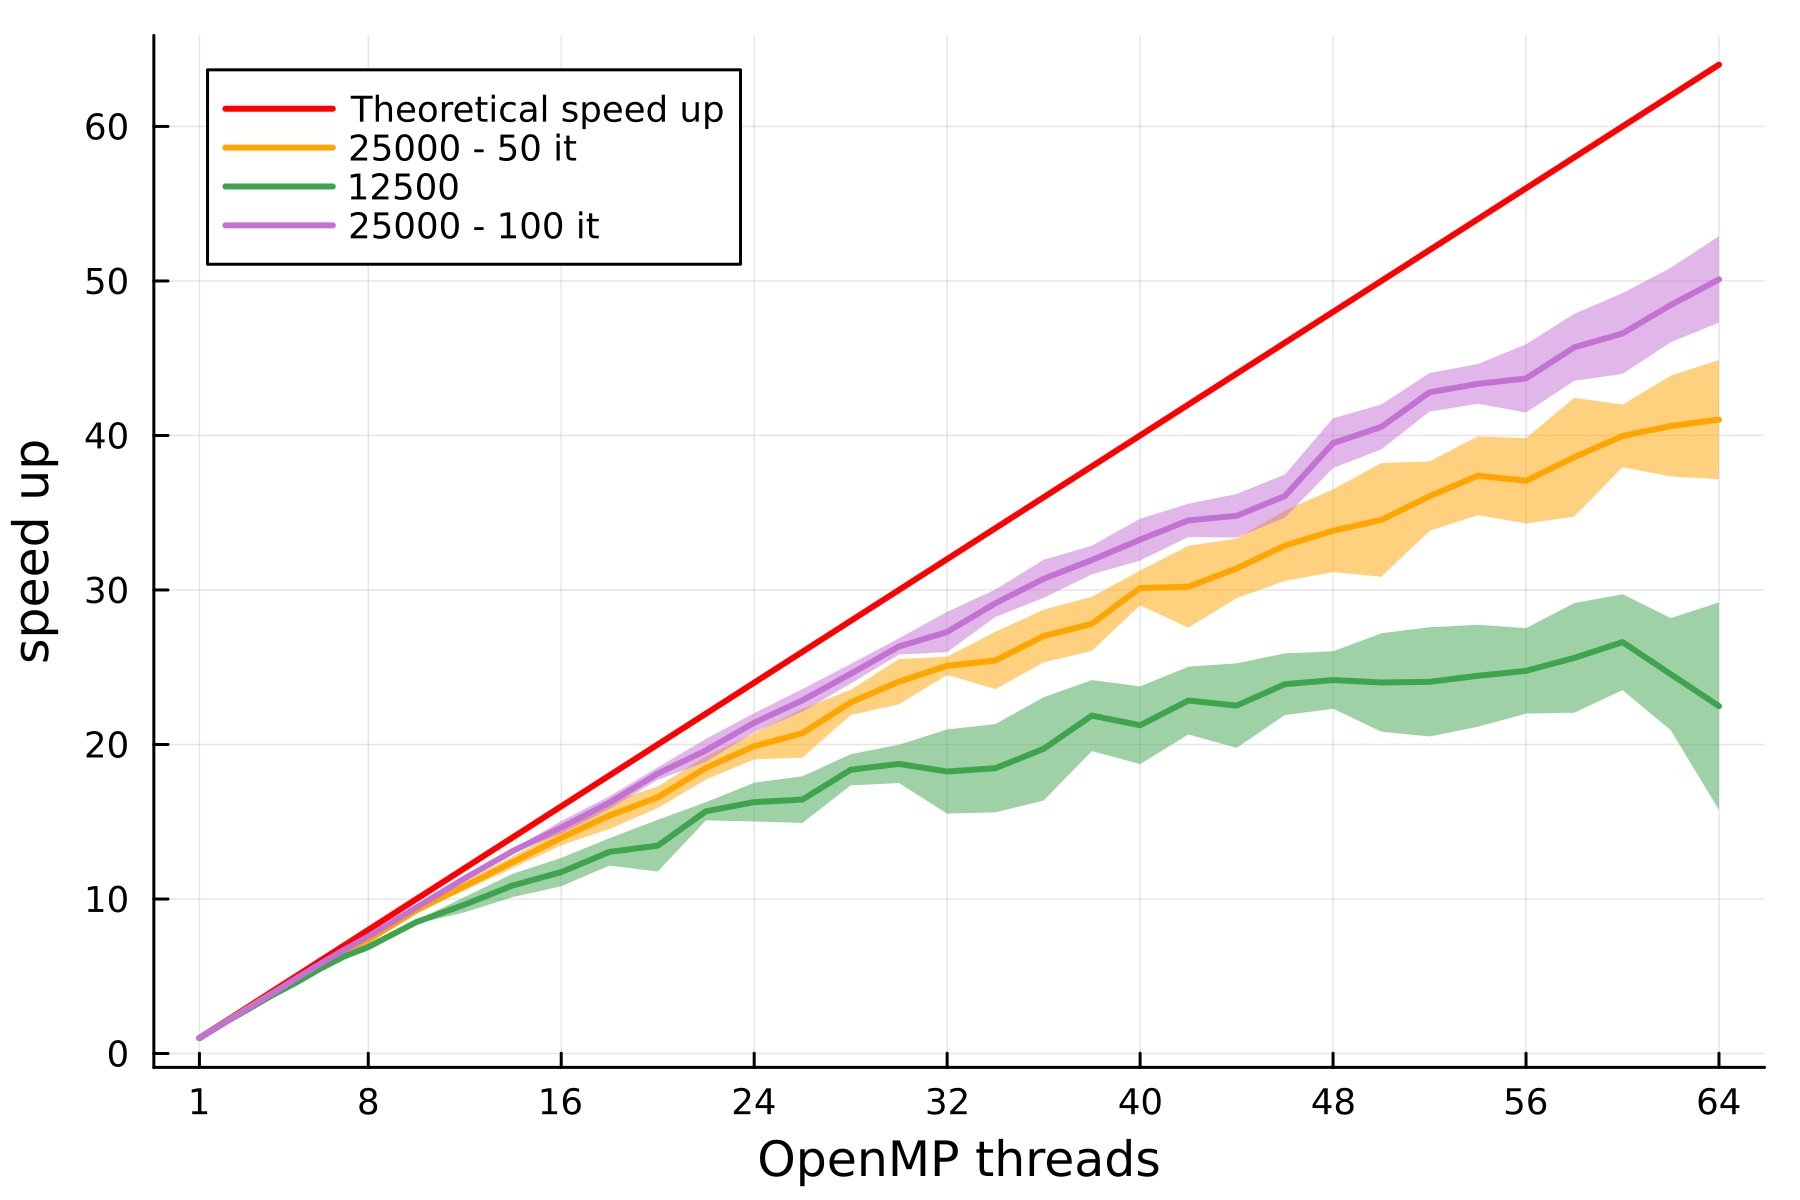
\includegraphics[width=\textwidth,height=3.64583in]{img/epyc_6_sockets.png}

}

\caption{OpenMP scalability - 6 sockets}

\end{figure}

\begin{figure}

{\centering 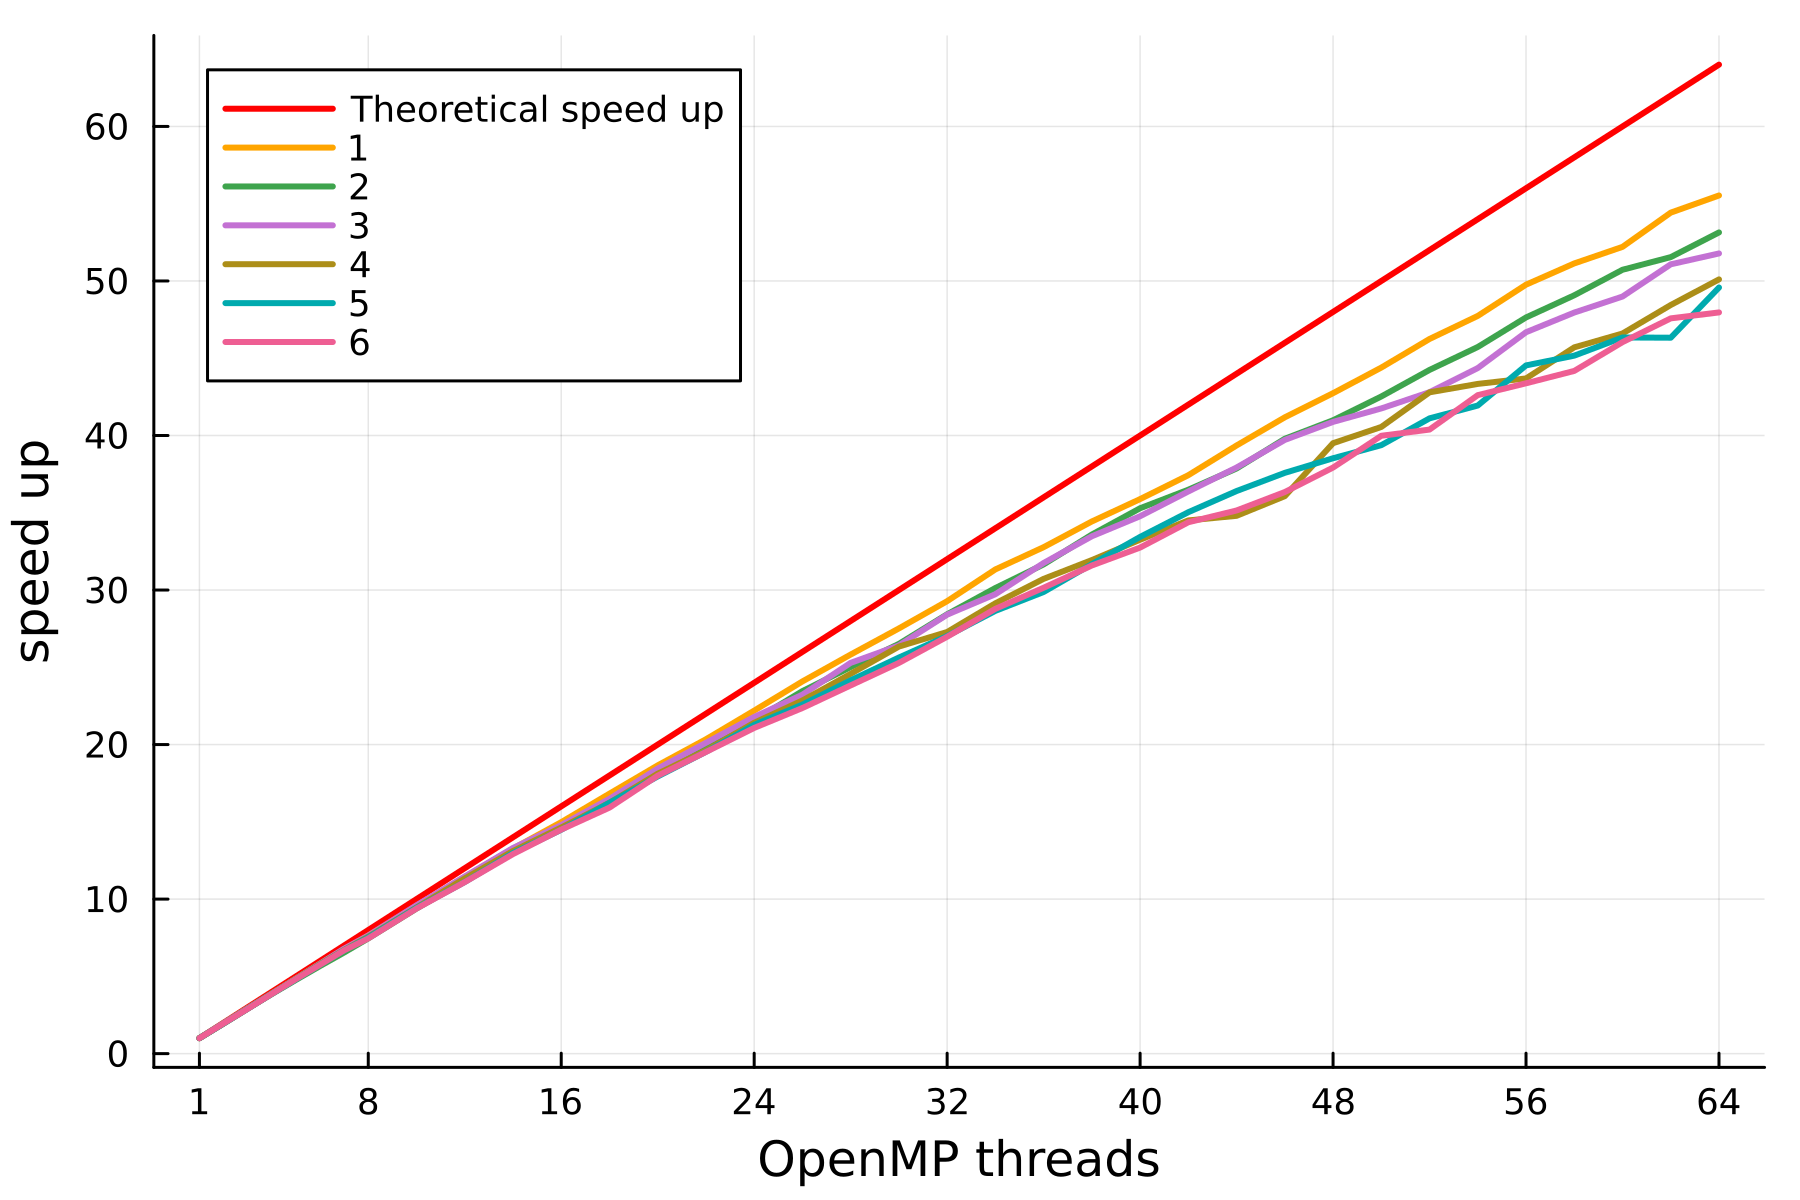
\includegraphics[width=\textwidth,height=3.64583in]{img/epyc_comparison.png}

}

\caption{OpenMP scalability - comparison matrix 25000x25000, 100 it}

\end{figure}

\newpage

As we can see from all the plots we have that as the workload increases,
the speed up increases too. We can also see that as the number of MPI
cores increases the speedup decreses. For example if we consider on epyc
node the line of the matrix of size \(25000\times 25000\) the speedup at
64 OpenMP threads with 1 MPI Task is about 52 indeed for 6 MPI Task the
speed up is around 48 (Figure{[}10{]}). This difference is even larger
if we consider the other two cases.

For the Thin node I have tested different two sizes of the matrix with
different number of iterations:

\begin{itemize}
\tightlist
\item
  Size: \(12500\times 12500\) and 50 iterations
\item
  Size: \(12500\times 12500\) and 100 iterations
\item
  Size \(62500\times 62500\) and 50 iterations
\end{itemize}

Below the graph of the scalability for the thin nodes:

\begin{figure}

{\centering 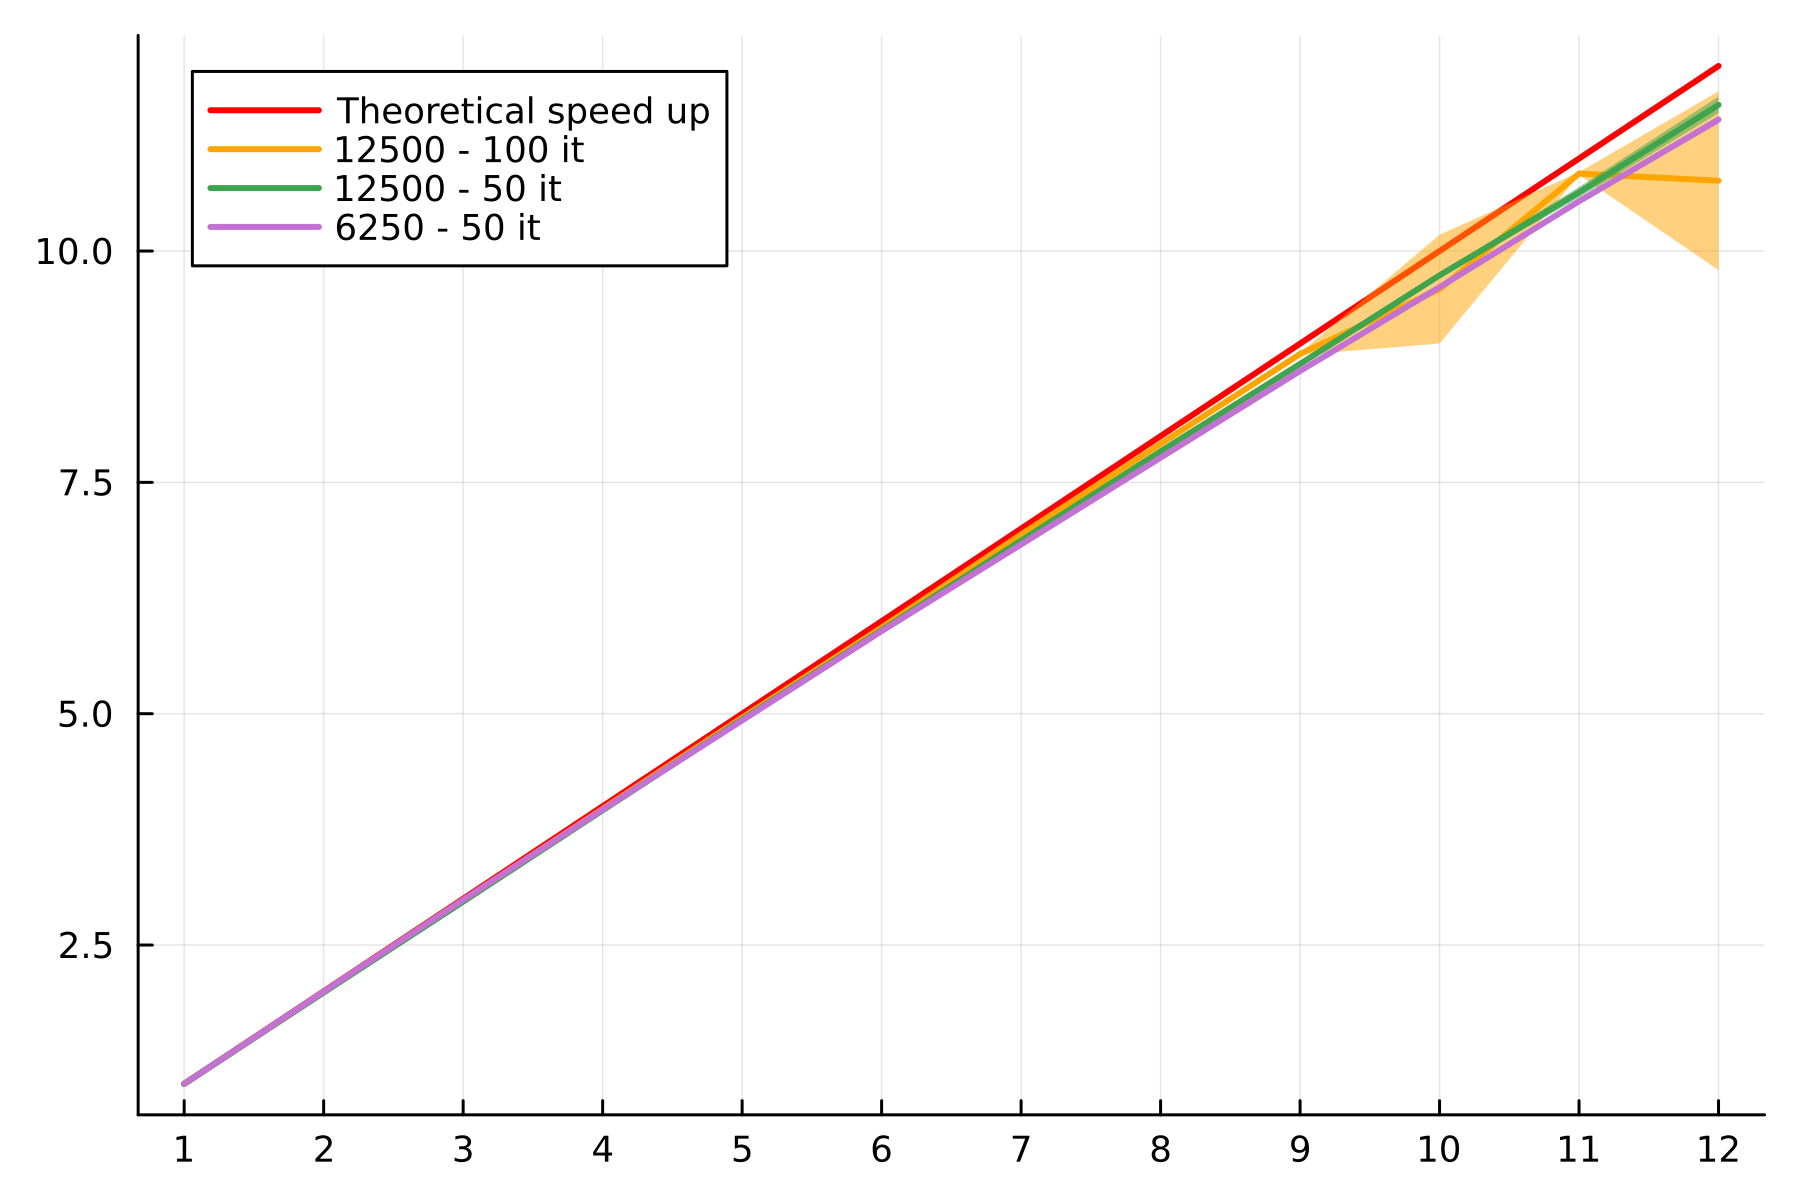
\includegraphics[width=\textwidth,height=3.64583in]{img/thin_1_socket.png}

}

\caption{OpenMP scalability Thin - 1 socket}

\end{figure}

\begin{figure}

{\centering 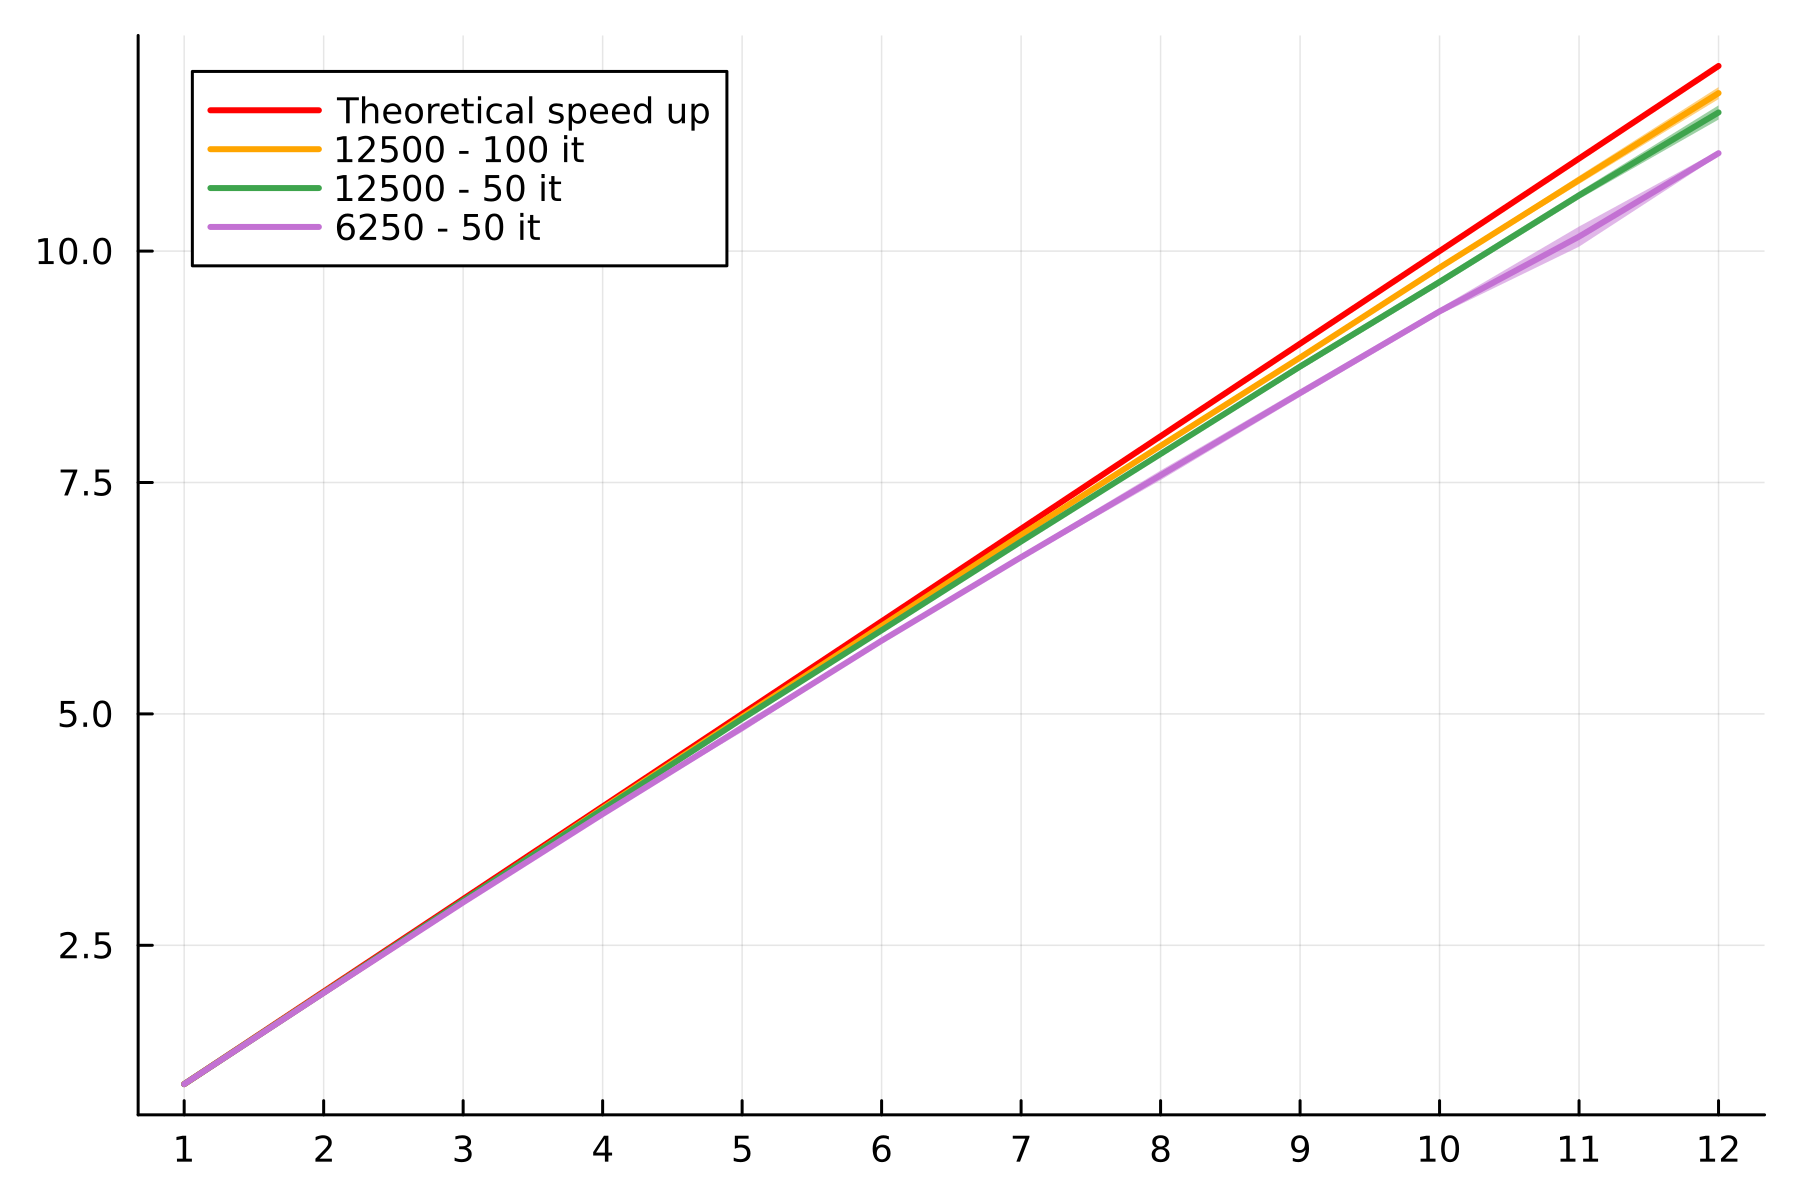
\includegraphics[width=\textwidth,height=3.64583in]{img/thin_2_sockets.png}

}

\caption{OpenMP scalability Thin - 2 sockets}

\end{figure}

\begin{figure}

{\centering 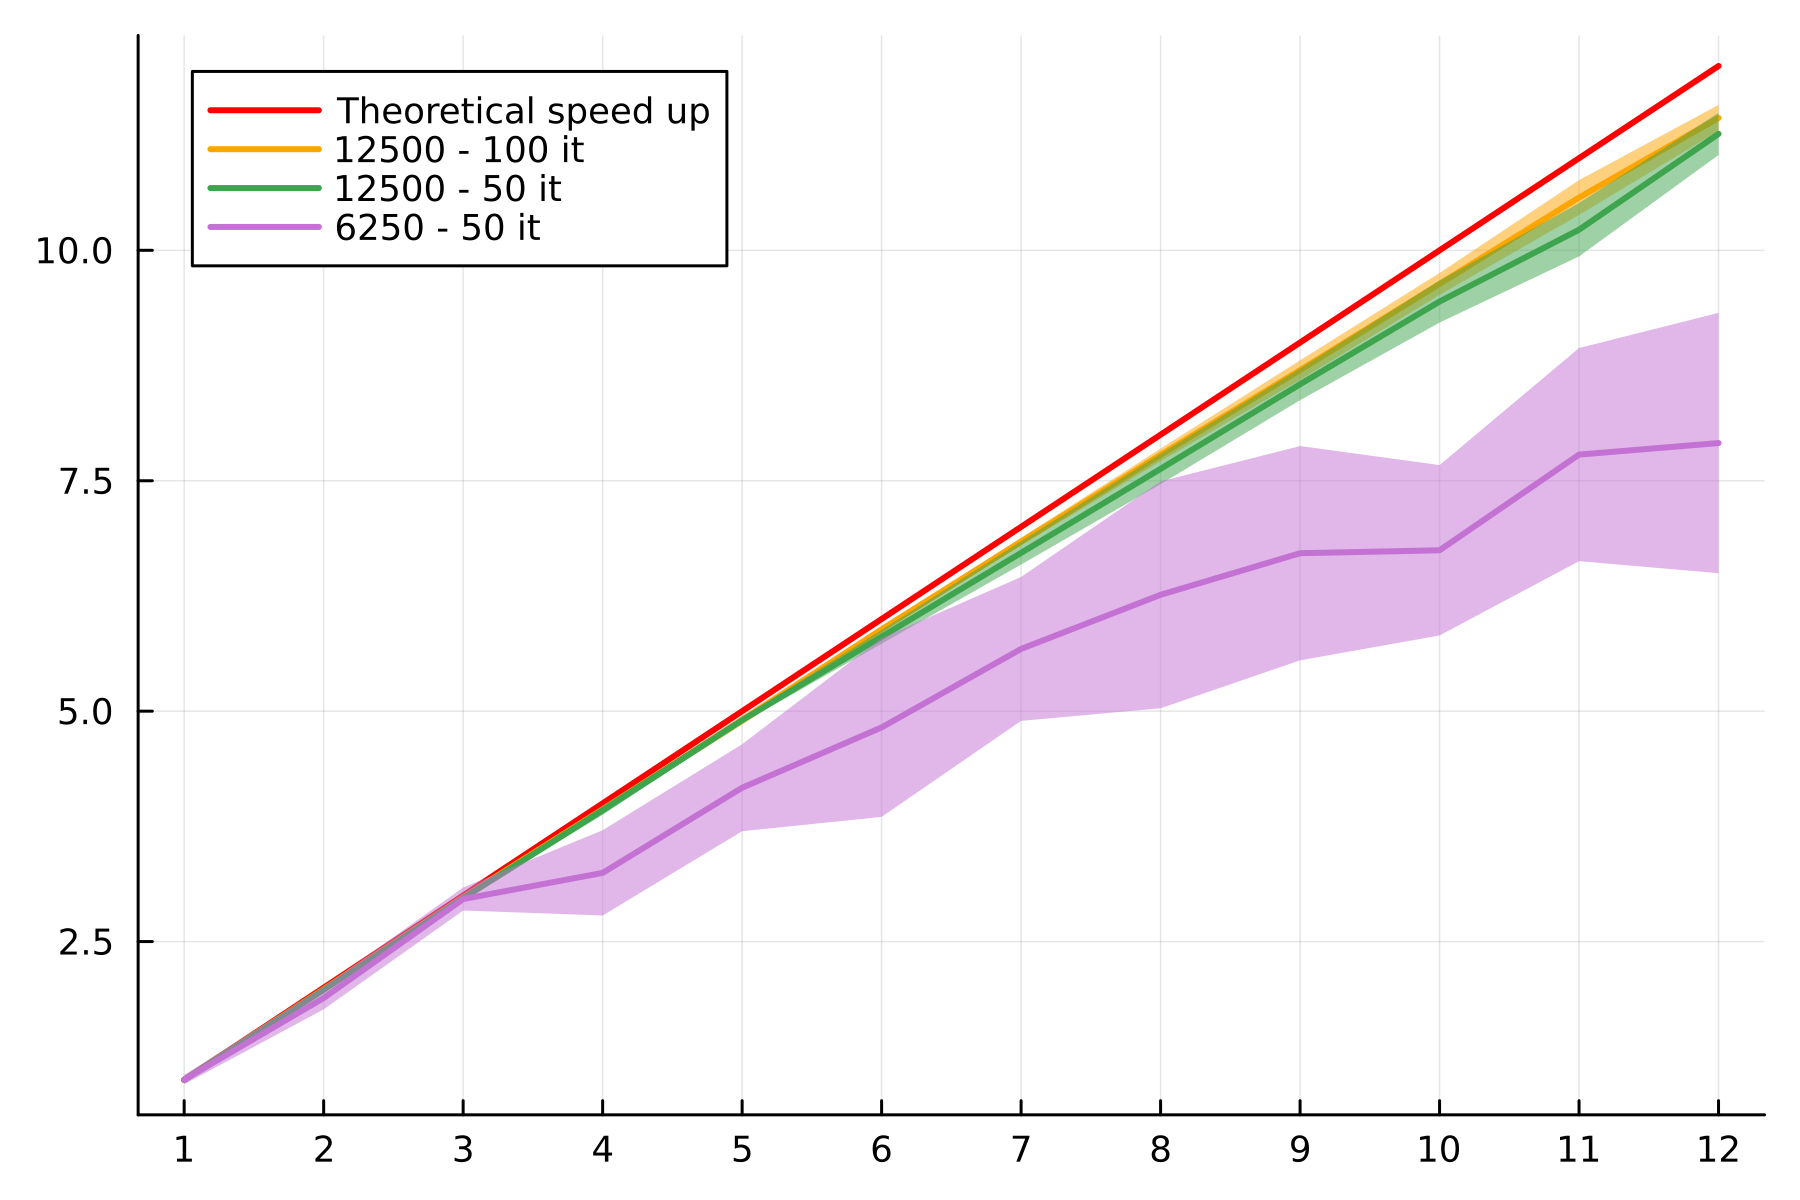
\includegraphics[width=\textwidth,height=3.64583in]{img/thin_3_sockets.png}

}

\caption{OpenMP scalability Thin - 3 sockets}

\end{figure}

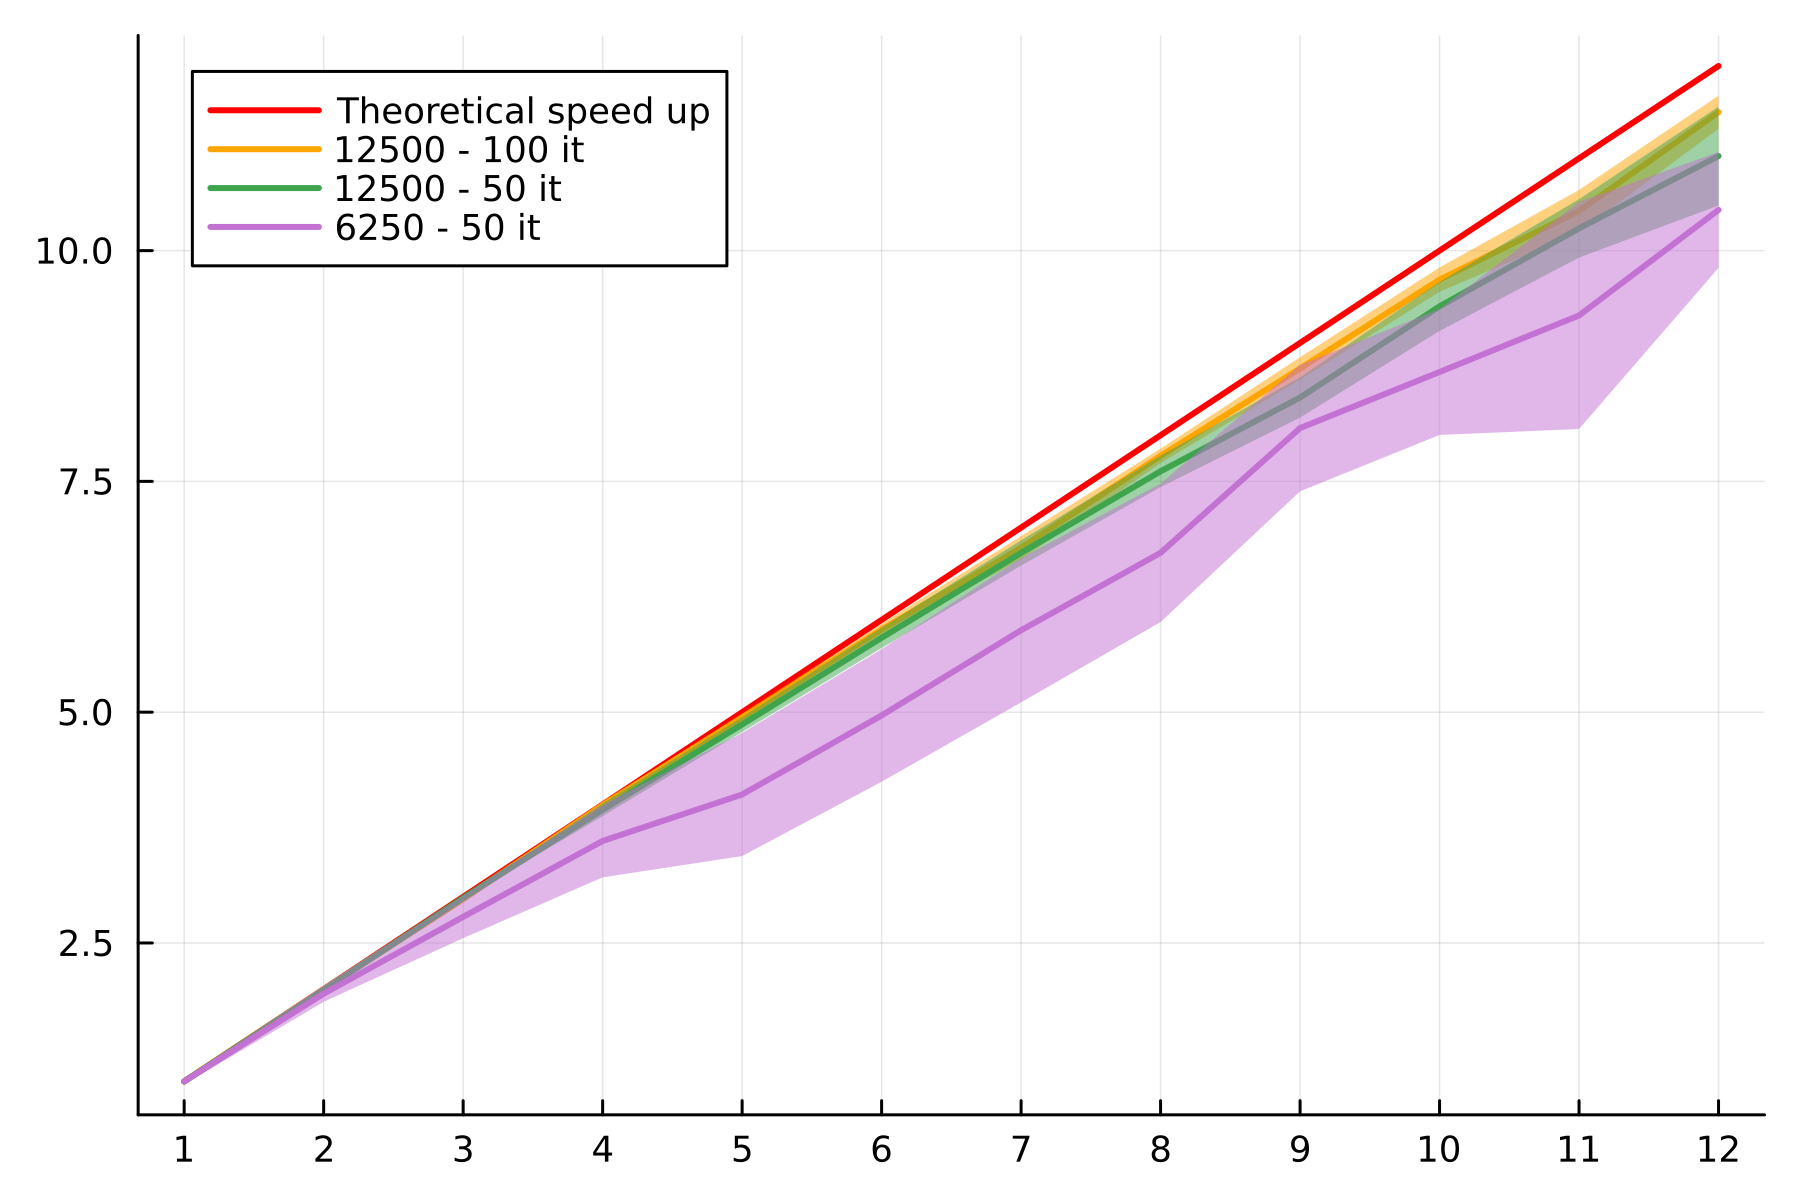
\includegraphics[width=\textwidth,height=3.64583in]{img/thin_4_sockets.png}
\newpage

All the observations made for Epyc nodes are valid, even, on the Thin
nodes

\hypertarget{mpi-weak-scalability}{%
\paragraph{MPI weak scalability}\label{mpi-weak-scalability}}

In this section the main idea is to mantain the workload for each MPI
Task constant. For this purpose I have decided to increase the size of
the matrix: the workload is basically determine by the size of the
matrix that each MPI Task has to work on. The formula that I have used
to determine the size of the matrix is:

\[
x\cdot \frac{x}{n} = s_{serial}^2
\]

Where \(s_{serial}\) is the size of a column/row of the original world.
Below the size of the world that I have used for the analysis:

\begin{longtable}[]{@{}cc@{}}
\toprule()
MPI Tasks & Size \\
\midrule()
\endhead
1 & 10000 \\
2 & 14143 \\
3 & 17321 \\
4 & 20000 \\
5 & 22361 \\
6 & 24495 \\
\bottomrule()
\end{longtable}

Below two graphs (using respectively 1 OpenMP thread and 32 OpenMP
threads) that shows the time of elaboration for the different number of
MPI Tasks). More graphs of this kind are available on the github
repository. As expected we can see that the computation time is almost
constant.

\begin{figure}

{\centering 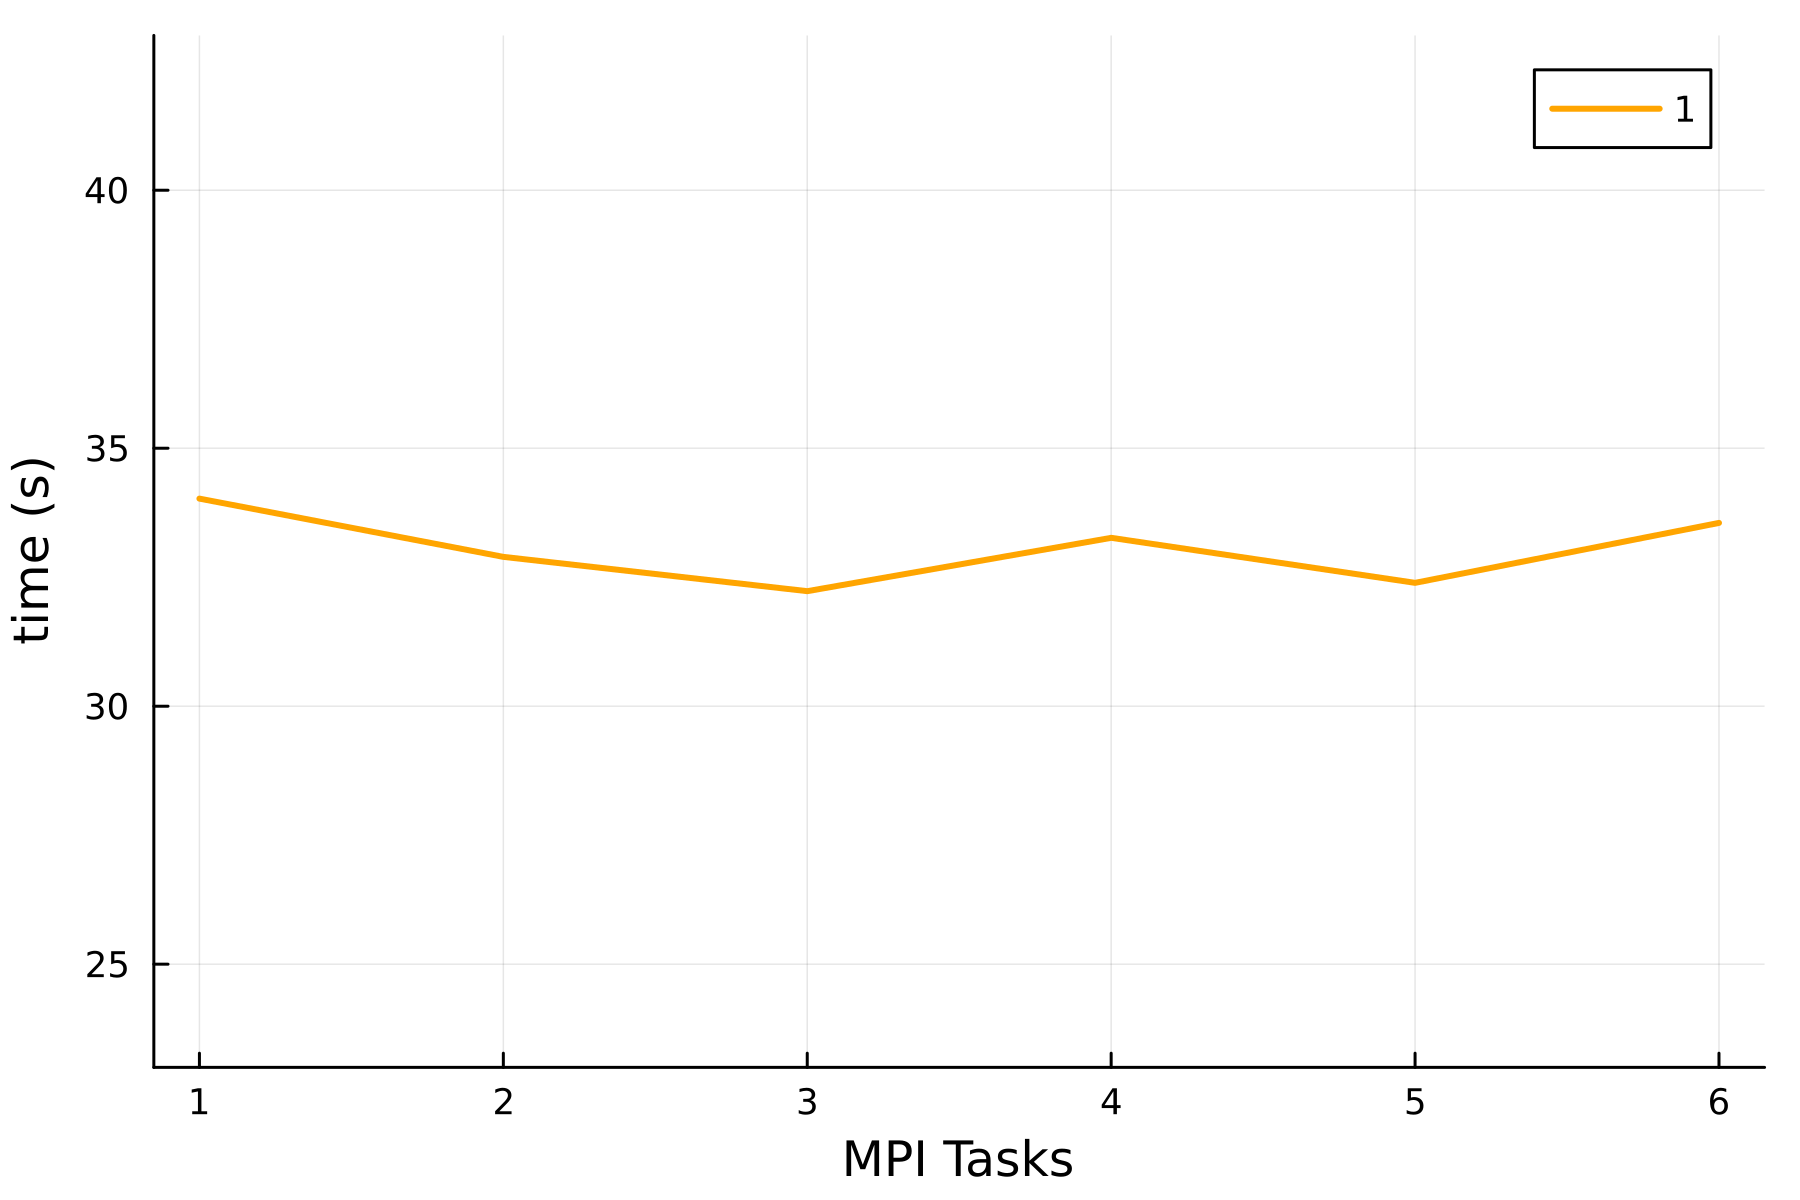
\includegraphics[width=\textwidth,height=3.64583in]{img/weak_scalability_mpi.png}

}

\caption{MPI Weak scalability - 1 OpenMP thread}

\end{figure}

\begin{figure}

{\centering 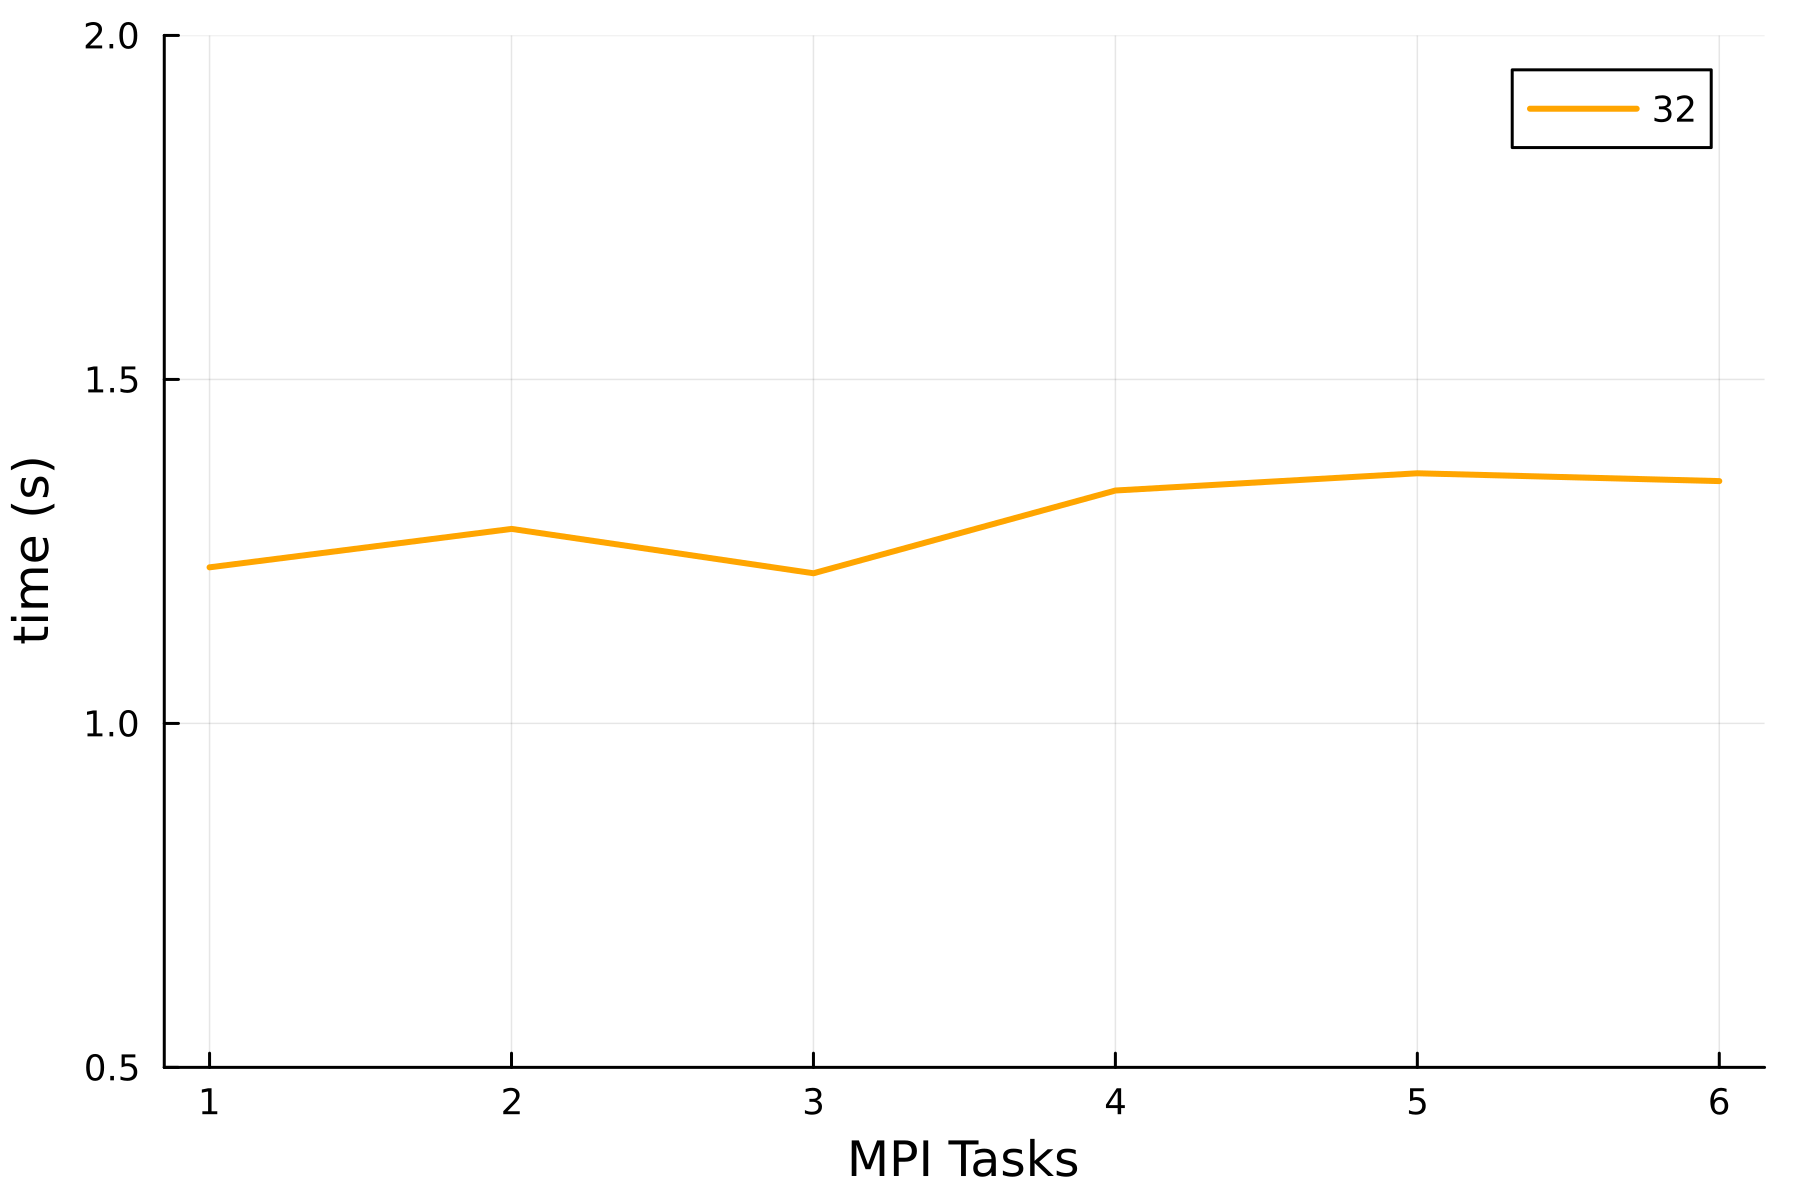
\includegraphics[width=\textwidth,height=3.64583in]{img/weak_scalability_mpi_32.png}

}

\caption{MPI Weak scalability - 32 OpenMP threads}

\end{figure}

\newpage

\hypertarget{strong-mpi-scalability}{%
\paragraph{Strong MPI scalability}\label{strong-mpi-scalability}}

In this section the main idea is to test how the code scales when the
number of MPI Tasks increses on a fixed size world. To do so I have run
the program using the option \texttt{-\/-map-by\ core} to place a
different MPI Task on each core. The test has been perform on epyc nodes
with the following parameters:

\begin{itemize}
\tightlist
\item
  Size=\(25000\times 250000\), it = 50
\item
  Size=\(25000\times 250000\), it = 100
\item
  Size=\(12500\times 125000\), it = 100
\end{itemize}

And on thin node with :

\begin{itemize}
\tightlist
\item
  Size \(12500\times 12500\) and 50 iterations
\item
  Size \(12500\times 12500\) and 100 iterations
\end{itemize}

Below the graphs:

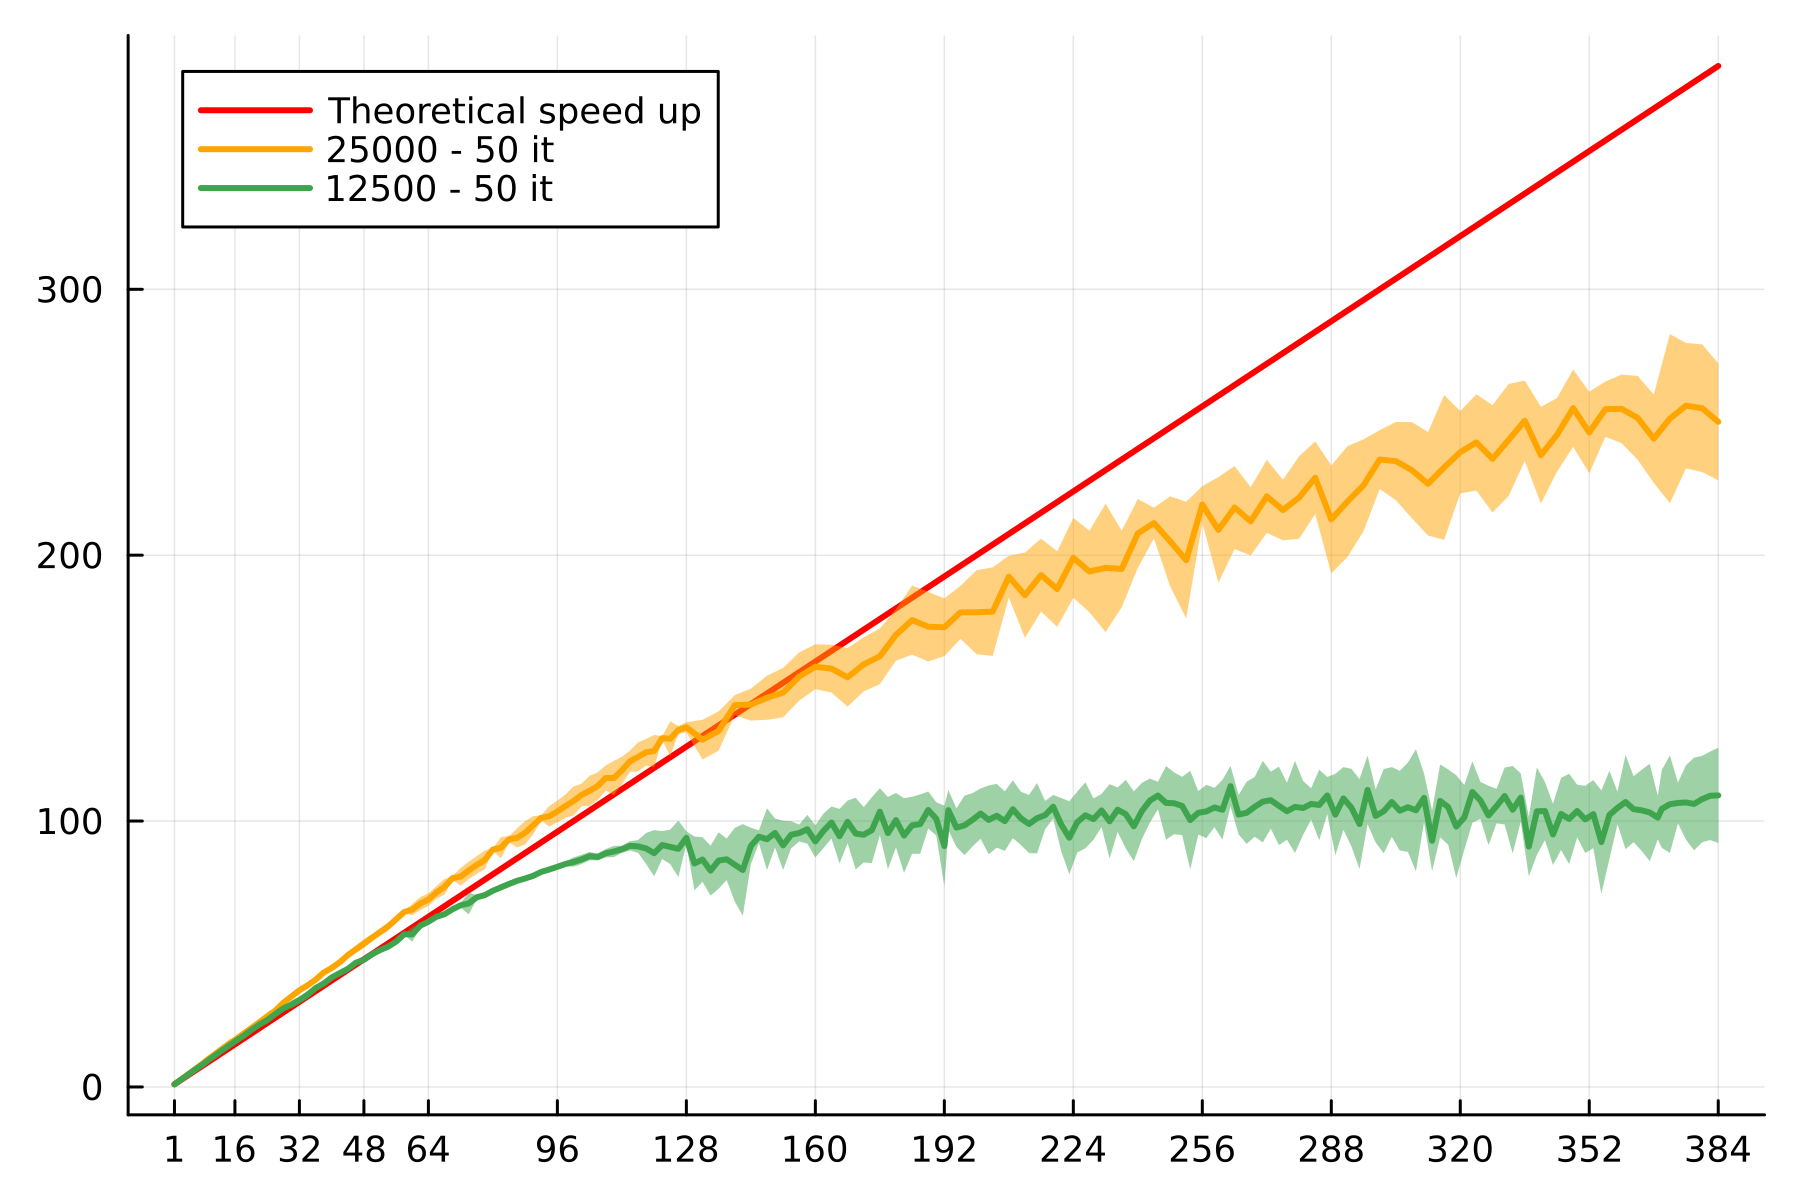
\includegraphics[width=\textwidth,height=3.64583in]{img/epyc_mpi_sockets.png}
\newpage

\begin{figure}

{\centering 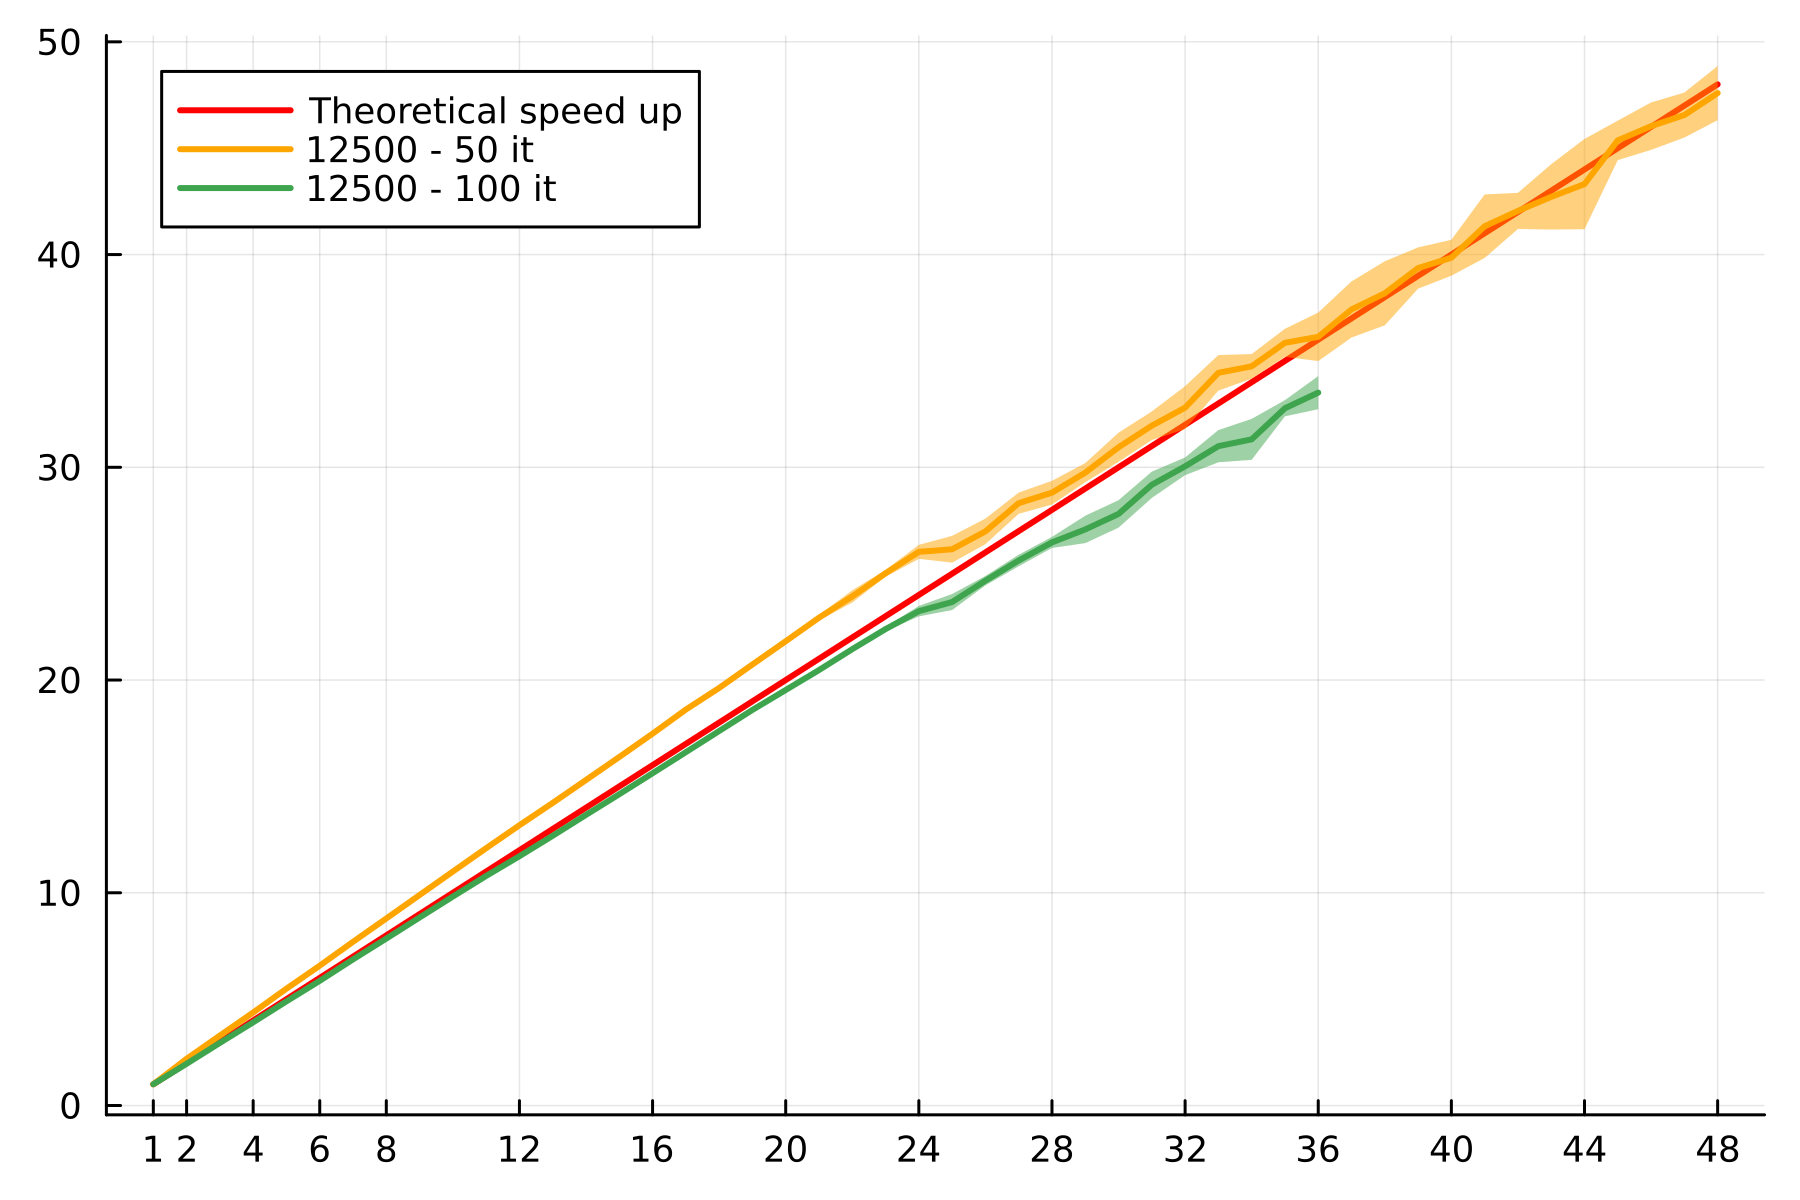
\includegraphics[width=\textwidth,height=3.64583in]{img/thin_mpi_sockets.png}

}

\caption{MPI Strong scalability - Thin}

\end{figure}

We can see, both on epyc and thin nodes, that before ``\emph{running
out}'' of the first node (48 MPI Tasks for thin and 128 MPI Tasks for
epyc) the speed up is above the ideal speed up. Another important thing
is that, similairly to the OpenMP scalability, the speedup is higher
when the workload is higher.

\hypertarget{iterate-ordered}{%
\subsubsection{Iterate ordered}\label{iterate-ordered}}

The program is strictly serial and, for this reason, I expect that the
elapsed time is constant, or increase due to parallelization overhead,
when we increases the numeber of MPI Tasks. Also a small increment on
the performances are not excluded due to better usage of the cache

\newpage

\begin{figure}

{\centering 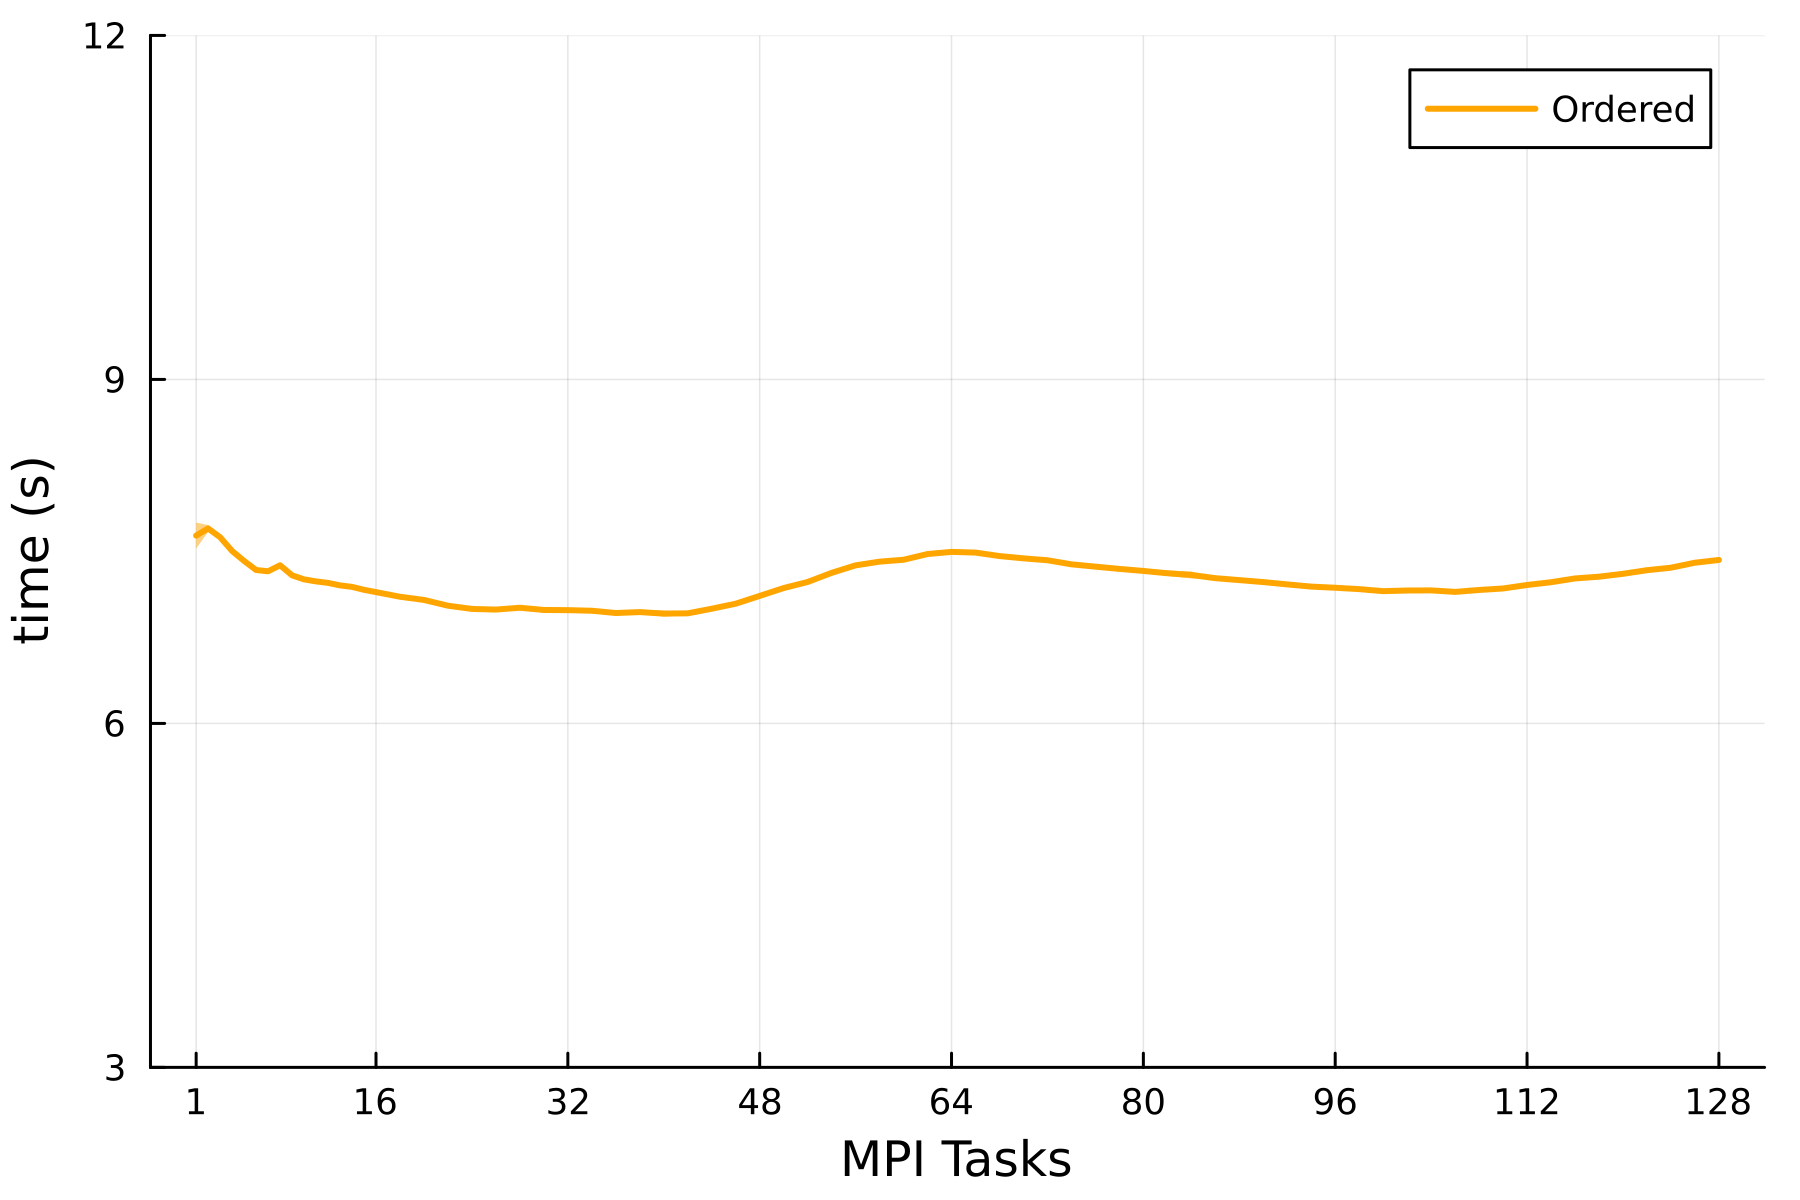
\includegraphics[width=\textwidth,height=3.64583in]{img/epyc_ordered.png}

}

\caption{Ordered Iteration - Epyc}

\end{figure}

\hypertarget{iterate-wave}{%
\subsubsection{Iterate wave}\label{iterate-wave}}

The test has been performed on a world of size \(10000 \times 10000\)
and 50 as number of iteration from 1 to 64 OpenMP threads. The OpenMP
options were \texttt{OMP\_PLACES=cores} end
\texttt{OMP\_PROC\_BIND=close}. The green in the plot below represent
the scalability when no numactl option have been set, while for the red
line I have used the following policy

\begin{itemize}
\tightlist
\item
  OpenMP threads from 1 to 16: \texttt{-\/-interleave=0}
\item
  OpenMP threads from 17 to 32: \texttt{-\/-interleave=0,1}
\item
  OpenMP threads from 33 to 48: \texttt{-\/-interleave=0,1,2}
\item
  OpenMP threads from 49 to 64: \texttt{-\/-interleave=0,1,2,3}
\end{itemize}

If we consider the green line we can se that the speed up is higher than
the theoretical one for the number of core in the range (14,36).
Something similar happen for the red line but fot the number of cores in
the range (16,24). We can also se that the speed up without the usage of
numactl is higher until 32 OpenMP threads. When we pass from 32 to 34
threads the speed up represented by the red line (wave iteration with
the usage of numactl) increase drastically.

\begin{figure}

{\centering 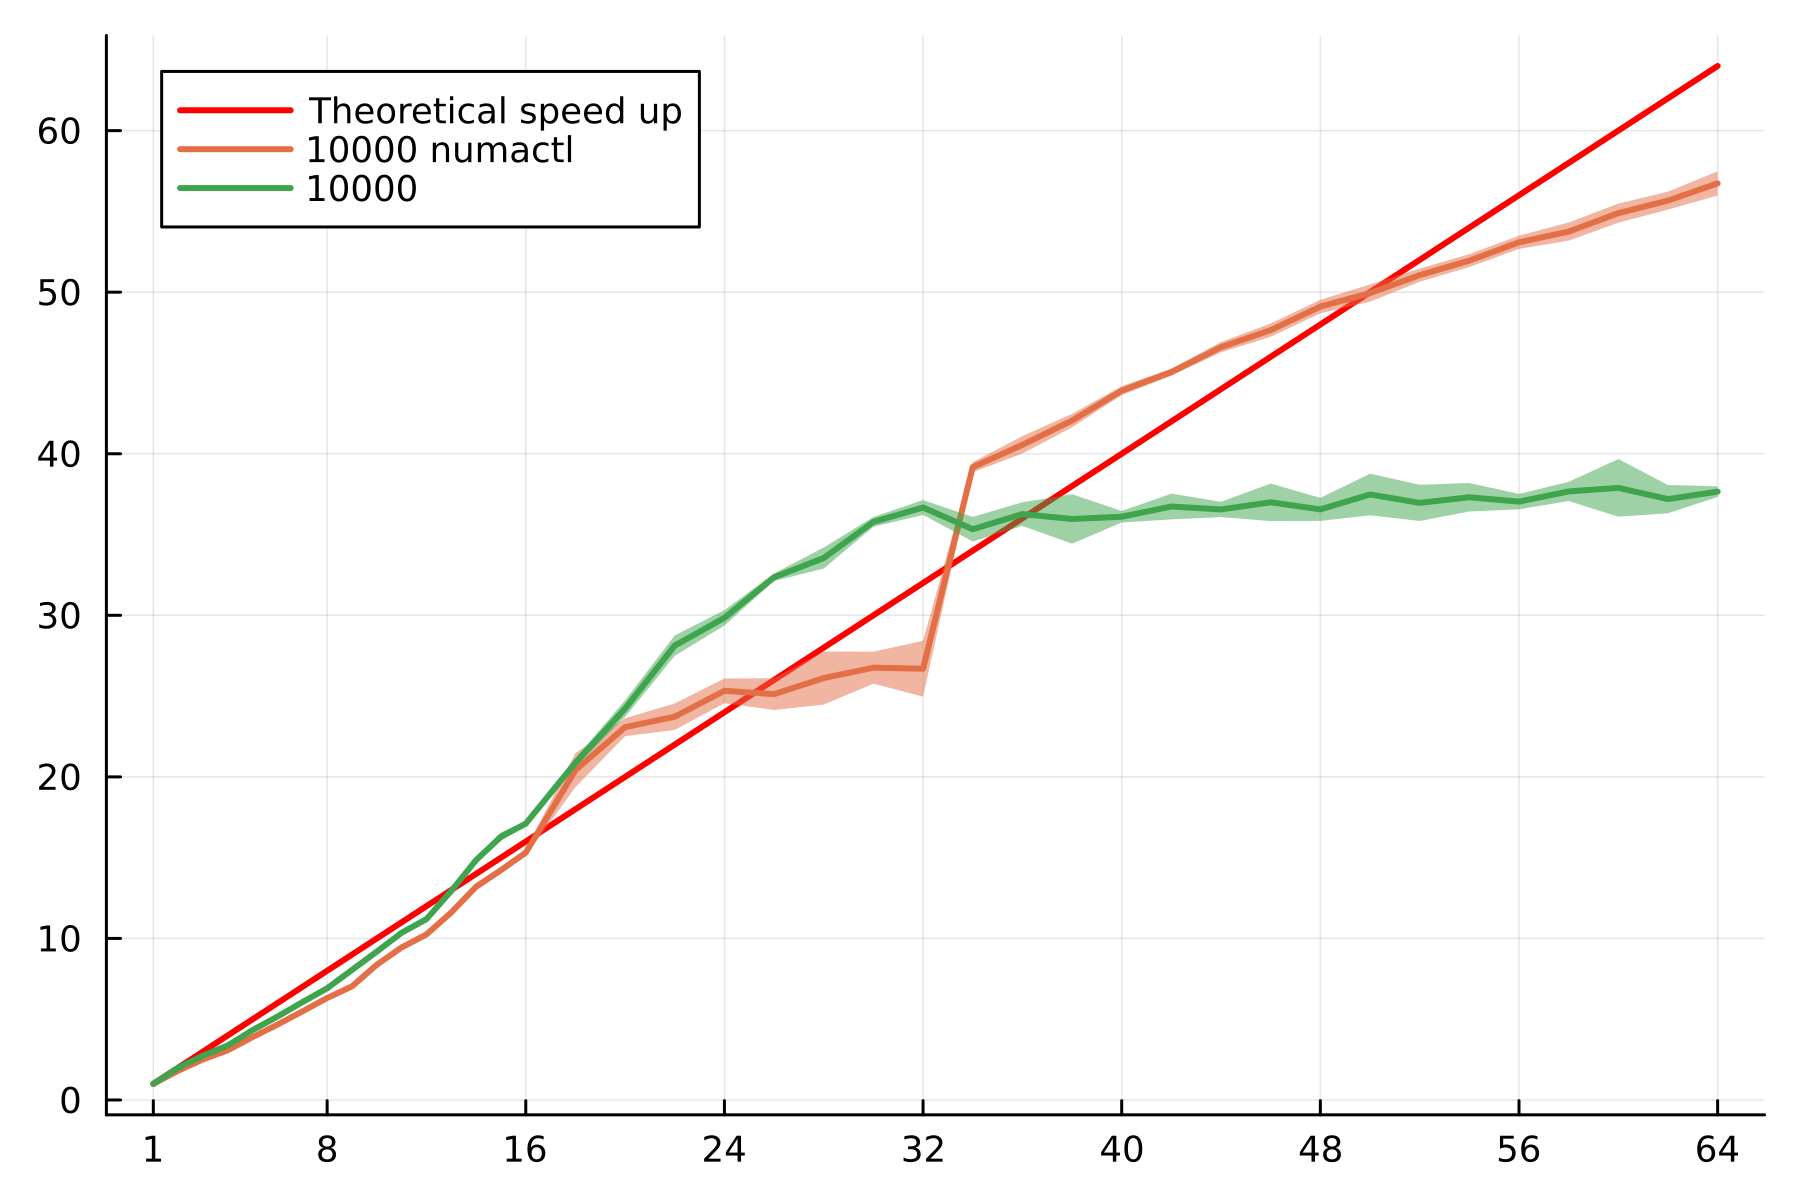
\includegraphics[width=\textwidth,height=3.64583in]{img/wave_scalability.png}

}

\caption{Wave Iteration - Epyc}

\end{figure}

\hypertarget{final-considerations}{%
\subsection{Final considerations}\label{final-considerations}}

At the end of this analysis I can say that program achived a good level
of scalability both in wave and static iteration methods. As it concerns
the ordered iteration my conclusion is that it is stricly serial and the
only possible parallelization is the one presented in the section above
which give as memory scalability.

Some possible improvements could be:

\begin{itemize}
\tightlist
\item
  Optimization of the writing procedure through MPI I/O.
\item
  Parallelize the reading from the file with openMP in order to improve
  also the memory allocation
\end{itemize}

\hypertarget{excercise-2}{%
\section{Excercise 2}\label{excercise-2}}

The goal of the excercise is to compare the performances of the math
libraries OpenBlas, Blis and MKL on the epyc node. The metric that has
been used to compare the performances is the number of floating point
operations per second, measured in GFlops. We are mainly intrestated in
analyzing the size scaling and the core scaling of the three algotithms.
To achive the goal I have used a slightly modified version of the code
\texttt{dgemm.c} present in the Assignment folder.

\hypertarget{size-scaling}{%
\subsection{Size scaling}\label{size-scaling}}

For the size scaling I have increased the size of the matrix from
\(2000 \times 20000\) to \(20000 \times 20000\) by steps of \(500\) (at
each step I have increased both the number of rows and the numbrer of
columns in order to have always square matrices). For each size and math
library I have taken 10 different measurment.

Below the tested policies (default options:
\texttt{OMP\_NUM\_THREADS=64} and \texttt{OMP\_PLACES=cores}):

\begin{itemize}
\tightlist
\item
  \texttt{OMP\_PROC\_BIND=close}, no numaclt options
\item
  \texttt{OMP\_PROC\_BIND=close}, \texttt{-\/-interleave=0,1,2,3}
\item
  \texttt{OMP\_PROC\_BIND=spred}, no numaclt options
\item
  \texttt{OMP\_PROC\_BIND=close},
  \texttt{-\/-interleave=0,1,2,3,4,5,6,7}
\end{itemize}

\hypertarget{single-precison}{%
\subsubsection{Single precison}\label{single-precison}}

The theoretical peak performance for a single socket on an epyc node is:

\[
P = n. cores\cdot frequency \cdot \frac{FLOPC}{cycle} = 64\cdot 2.6 GHz\cdot 32 Flops = 5324,8 GFlops
\]

A AMD Epyc 7H12 (the one that we can find on orfeo cluster) can deliver
16 double precision \(\frac{FLOPS}{cycle}\) and 32 single precision
\(\frac{FLOPS}{cycle}\)

The table below shows the peak performances:

\begin{longtable}[]{@{}
  >{\raggedright\arraybackslash}p{(\columnwidth - 12\tabcolsep) * \real{0.3725}}
  >{\raggedright\arraybackslash}p{(\columnwidth - 12\tabcolsep) * \real{0.0980}}
  >{\raggedright\arraybackslash}p{(\columnwidth - 12\tabcolsep) * \real{0.1471}}
  >{\raggedright\arraybackslash}p{(\columnwidth - 12\tabcolsep) * \real{0.0882}}
  >{\raggedright\arraybackslash}p{(\columnwidth - 12\tabcolsep) * \real{0.1078}}
  >{\raggedright\arraybackslash}p{(\columnwidth - 12\tabcolsep) * \real{0.0882}}
  >{\raggedright\arraybackslash}p{(\columnwidth - 12\tabcolsep) * \real{0.0980}}@{}}
\toprule()
\begin{minipage}[b]{\linewidth}\raggedright
Settings
\end{minipage} & \begin{minipage}[b]{\linewidth}\raggedright
OpenBlas
\end{minipage} & \begin{minipage}[b]{\linewidth}\raggedright
Size OpenBlas
\end{minipage} & \begin{minipage}[b]{\linewidth}\raggedright
Blis
\end{minipage} & \begin{minipage}[b]{\linewidth}\raggedright
Size Blis
\end{minipage} & \begin{minipage}[b]{\linewidth}\raggedright
MKL
\end{minipage} & \begin{minipage}[b]{\linewidth}\raggedright
Size MKL
\end{minipage} \\
\midrule()
\endhead
close, no numactl & 2493.85 & 19500 & 2579.73 & 5500 & 2097.68 & 5500 \\
close, --interleave=0,1,2,3 & 3838.42 & 18500 & 3930.98 & 19500 &
2770.25 & 20000 \\
spread, no numactl & 2553.95 & 18000 & 2959.80 & 7500 & 2199.13 &
7000 \\
spread, --interleave=0,1,2,3,4,5,6,7 & 4444.82 & 19500 & 4314.61 & 19500
& 3042.04 & 7000 \\
\bottomrule()
\end{longtable}

\newpage

The graphs below represent the scaling of math library when the policy
changes (one graph for each policy). In all the three math libraries the
usage of numactl options improve the overall performance. This is
reasonable because of the lower average time that an OpenMP thread needs
to access the RAM (better memory allocation). We can also see, on blis
graph, that the curve of the policy spread with the usage of numactl,
has a local maximum for \(n=m=k=9000\). A possible explanation for this
behaviour cuold be linked to a optimal cache usage at those sizes.

\begin{figure}

{\centering 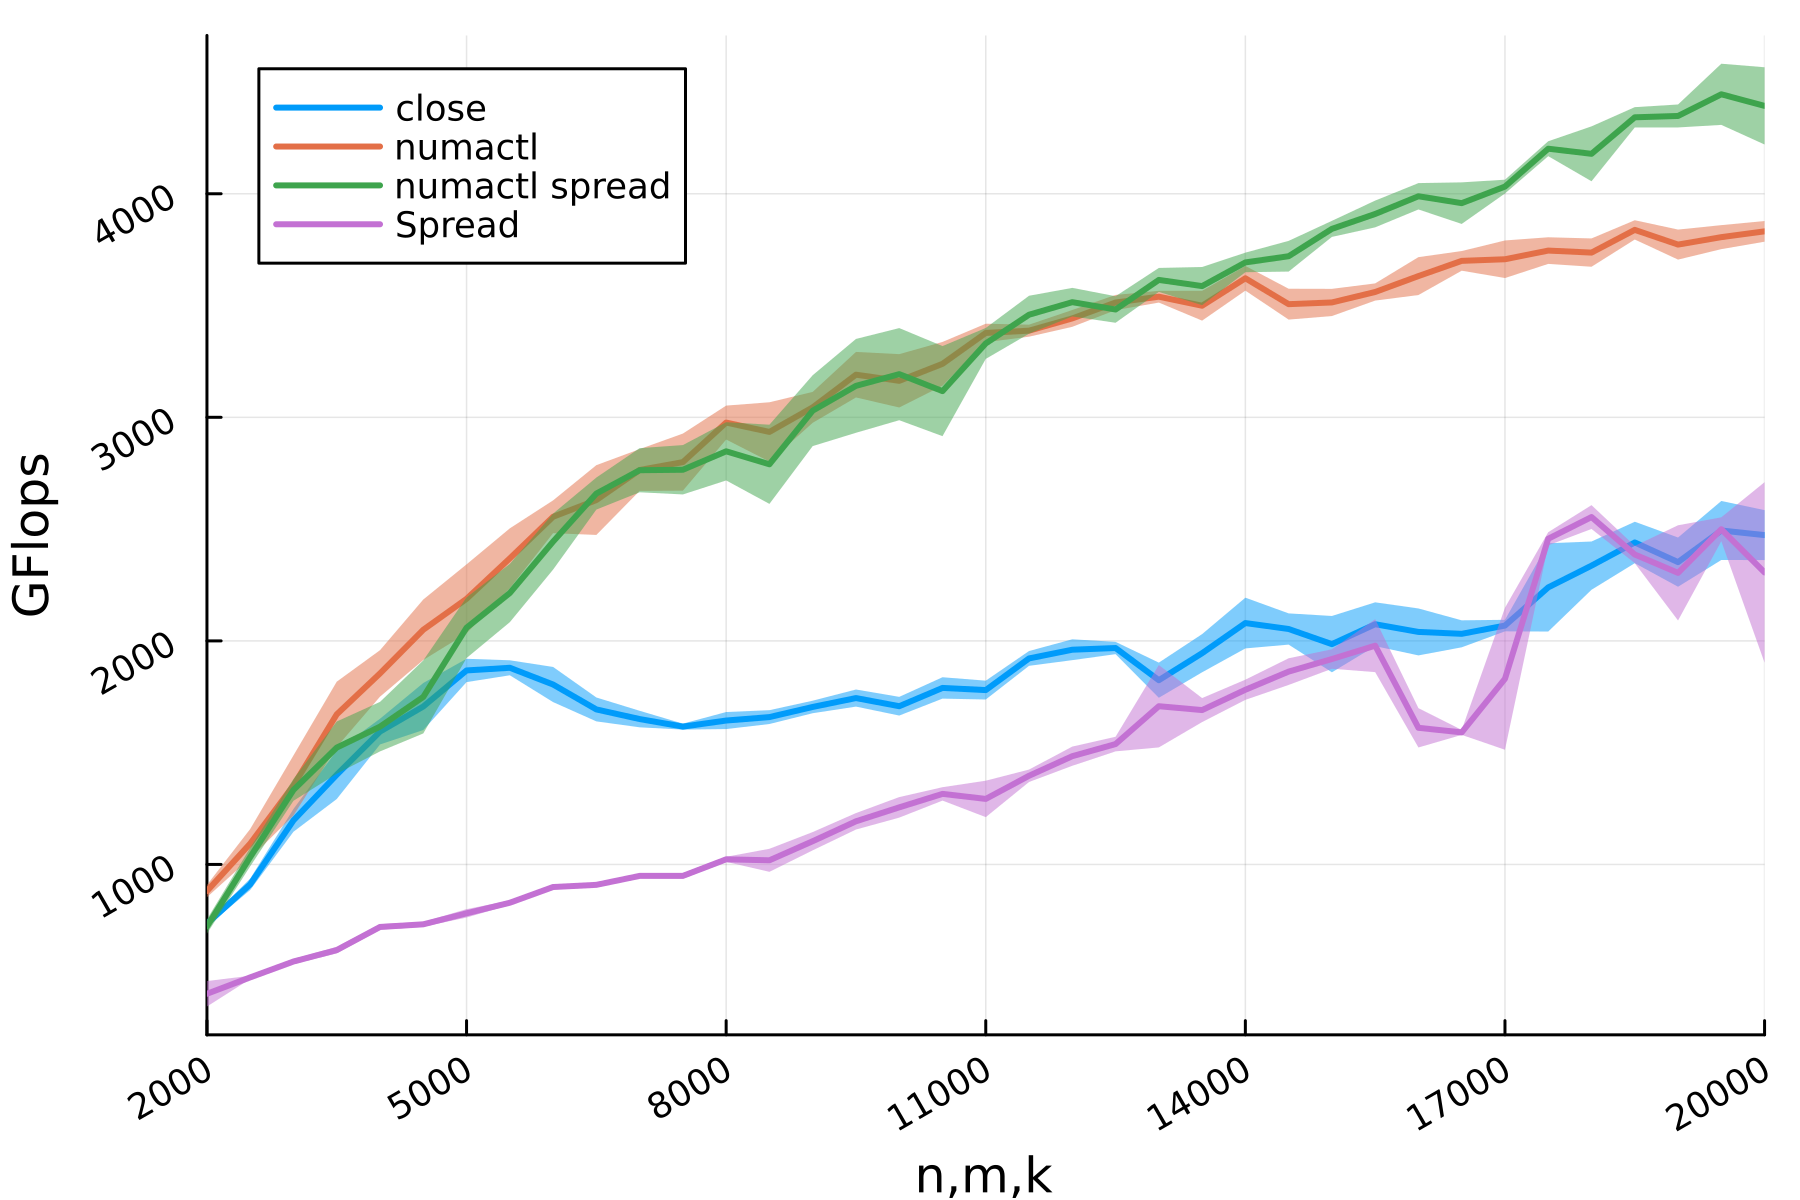
\includegraphics[width=\textwidth,height=3.64583in]{img/float_obals_comparison.png}

}

\caption{Comparison OpenBlas - Float}

\end{figure}

\begin{figure}

{\centering 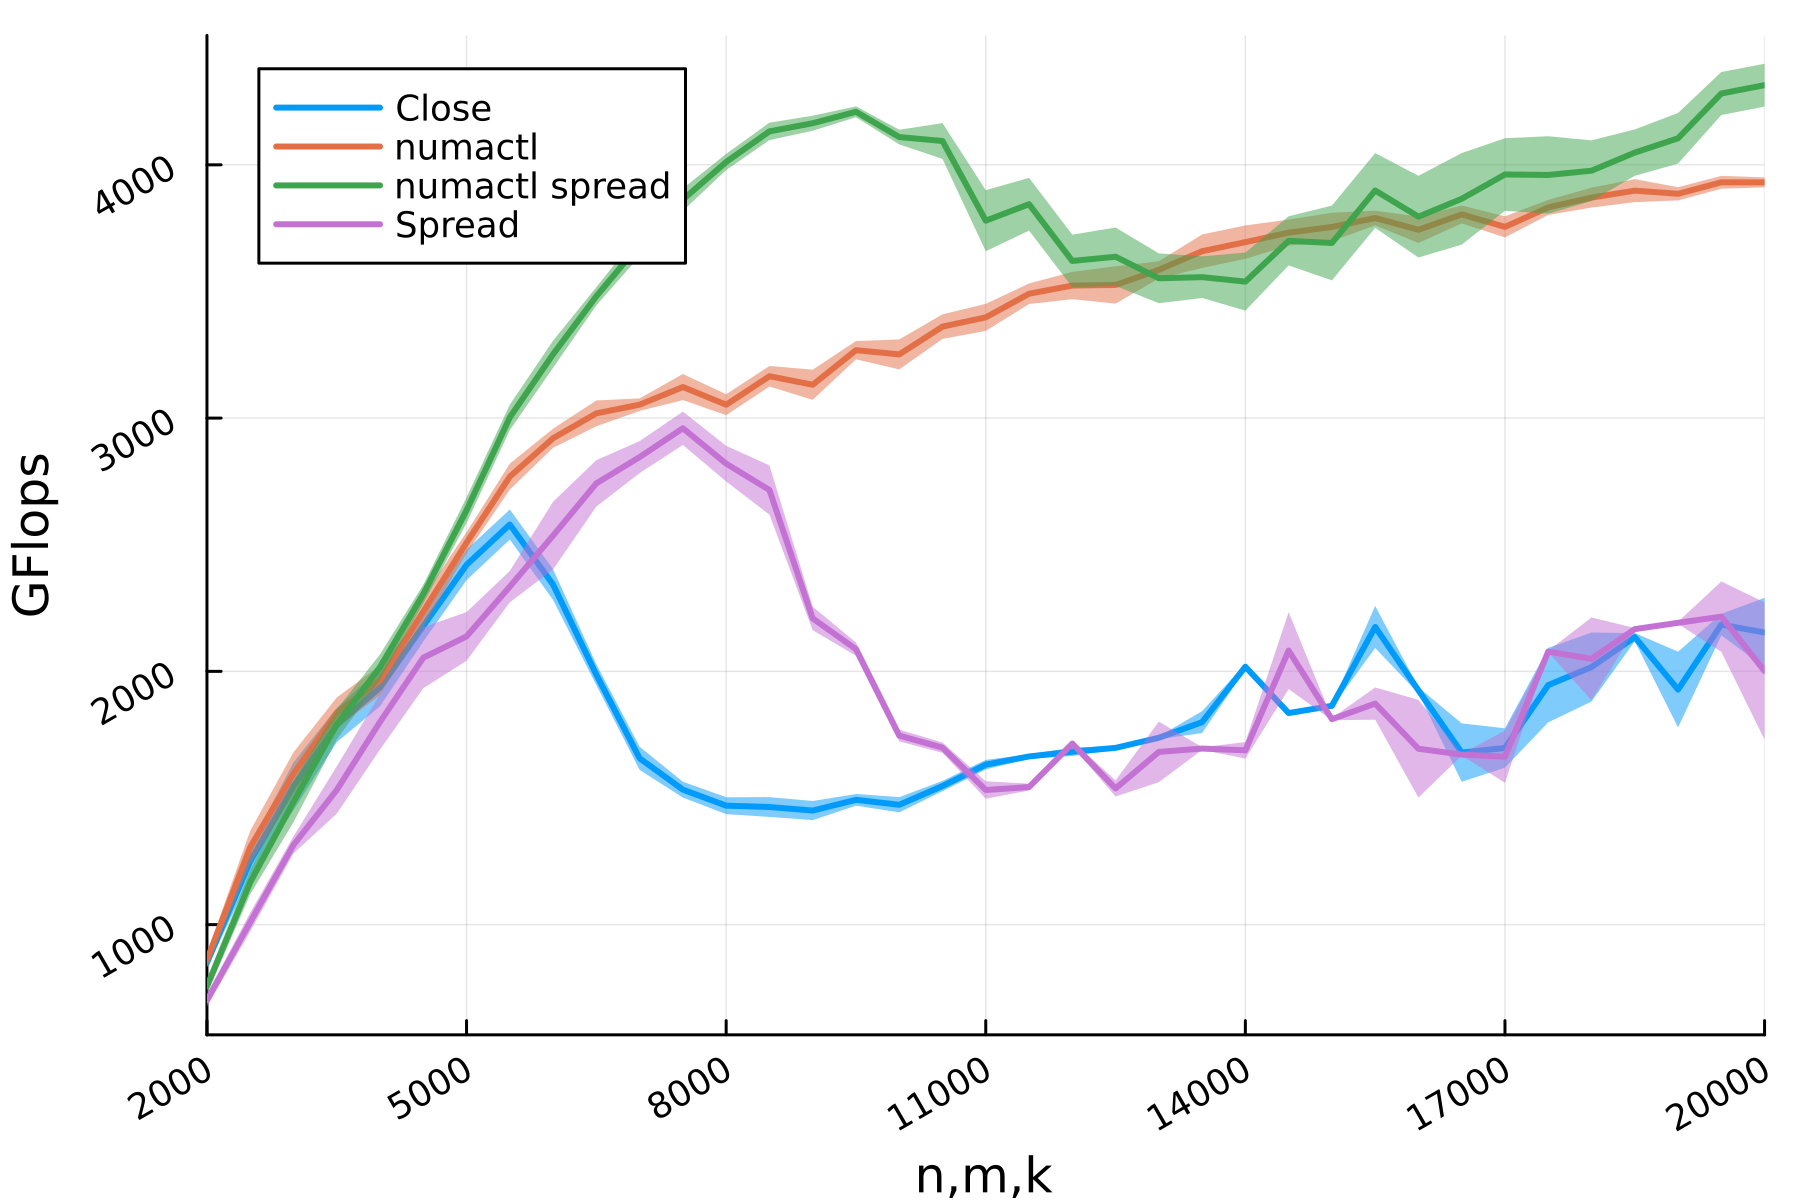
\includegraphics[width=\textwidth,height=3.64583in]{img/float_blis_comparison.png}

}

\caption{Comparison Blis - Float}

\end{figure}

\begin{figure}

{\centering 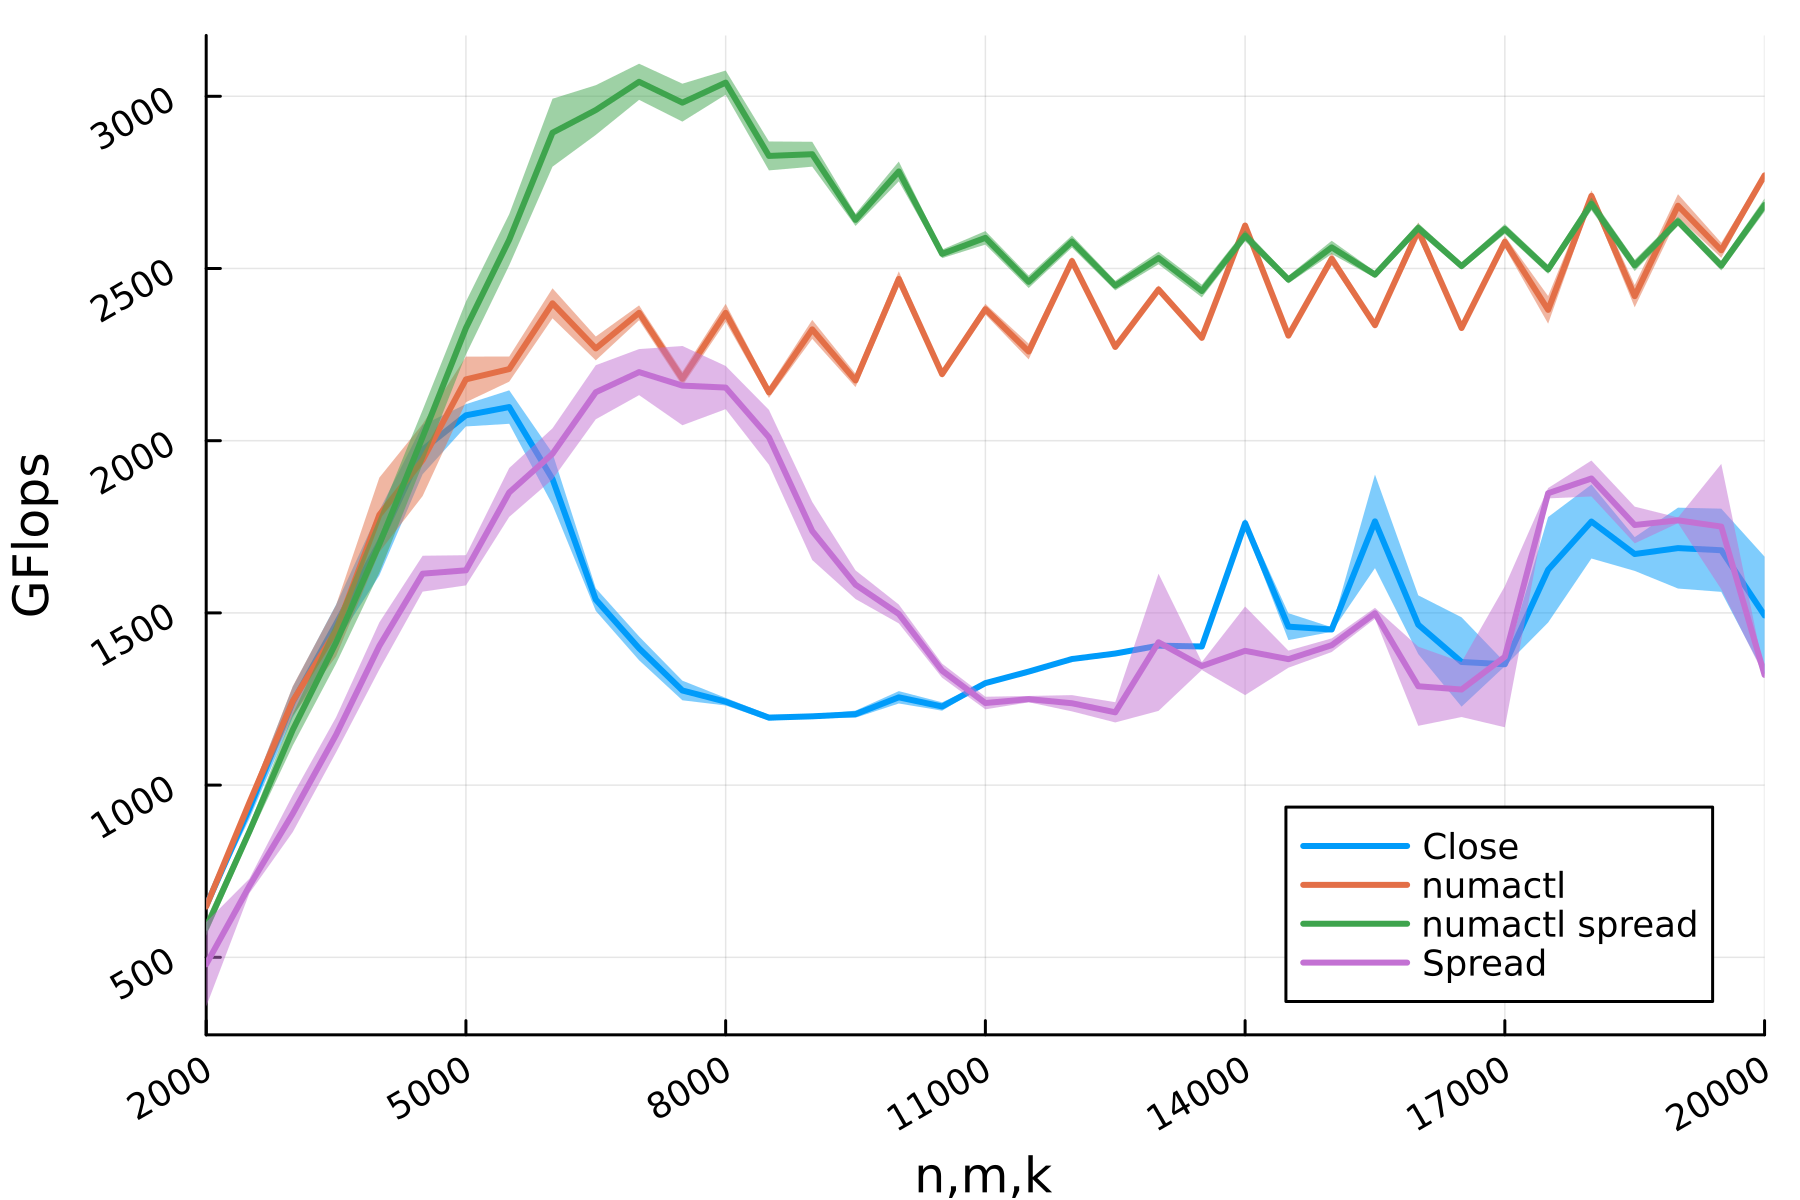
\includegraphics[width=\textwidth,height=3.64583in]{img/float_mkl_comparison.png}

}

\caption{Comparison MKL - Float}

\end{figure}

\newpage

In the graphs below I have gathered togheter the different math
libraries (one plot for each policy).

For the close policy with no numactl options we can see that at the
beggining Blis performs better then the other until \(n=m=k=5500\).
Starting from \(n=m=k=6000\) the GFlops of all the libraries fall down
until \(n=m=k=10000\). Note that from \(n=m=k=7000\) openBlas performs
better than Blis.

With the policy with \texttt{OMP\_PROC\_BIND=close} and
\texttt{numactl\ -\/-interleave=0,1,2,3} we have that Blis performs
slightly better than OpenBlas.

Finally with the policy \texttt{OMP\_PROC\_BIND=spread} and
\texttt{numactl\ -\/-interleave=0,1,2,3,4,5,6,7} Blis performs better
than the others from \(n=m=k=2000\) until \(n=m=k=1200\). After that
value Blis and OpenBlas are almost equivalent

\begin{figure}

{\centering 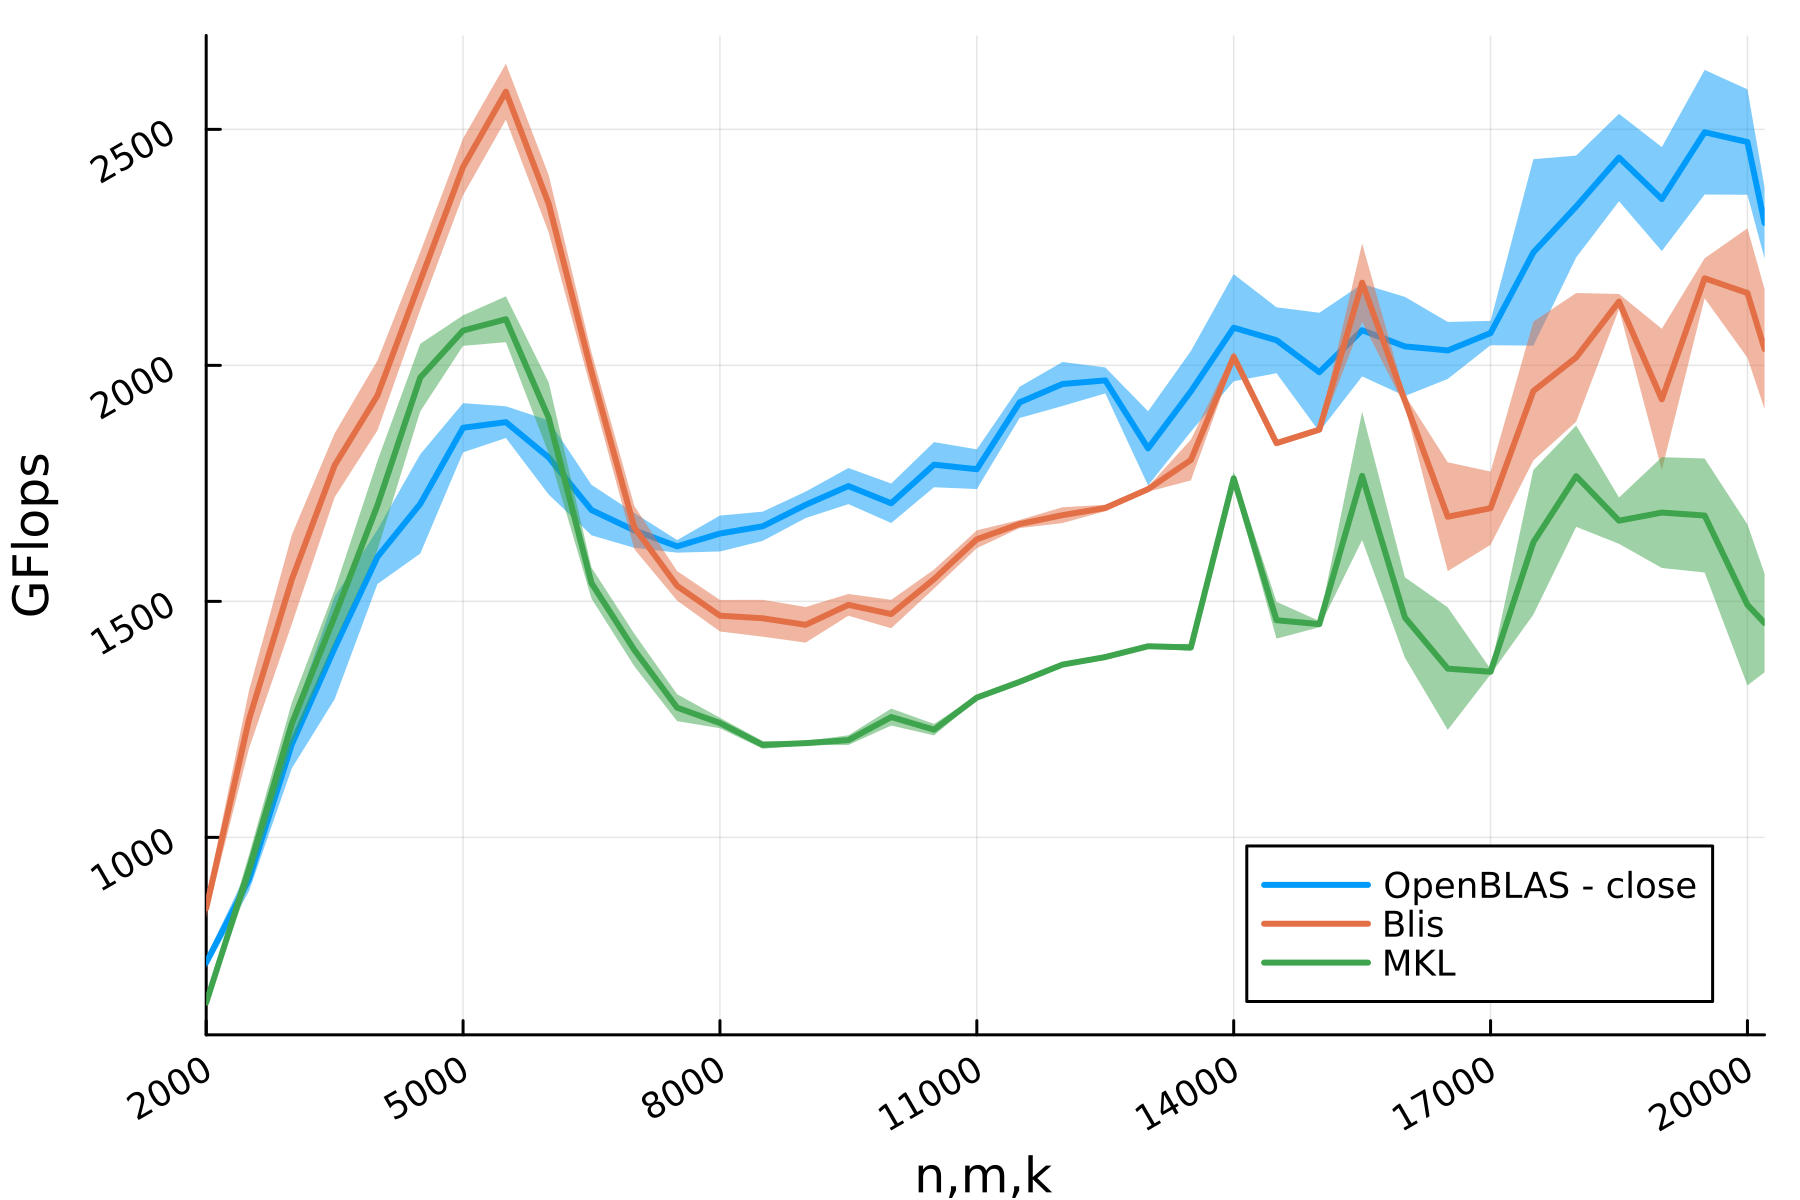
\includegraphics[width=\textwidth,height=3.64583in]{img/float_close_comparison.png}

}

\caption{Comparison close, no numactl options - Float}

\end{figure}

\begin{figure}

{\centering 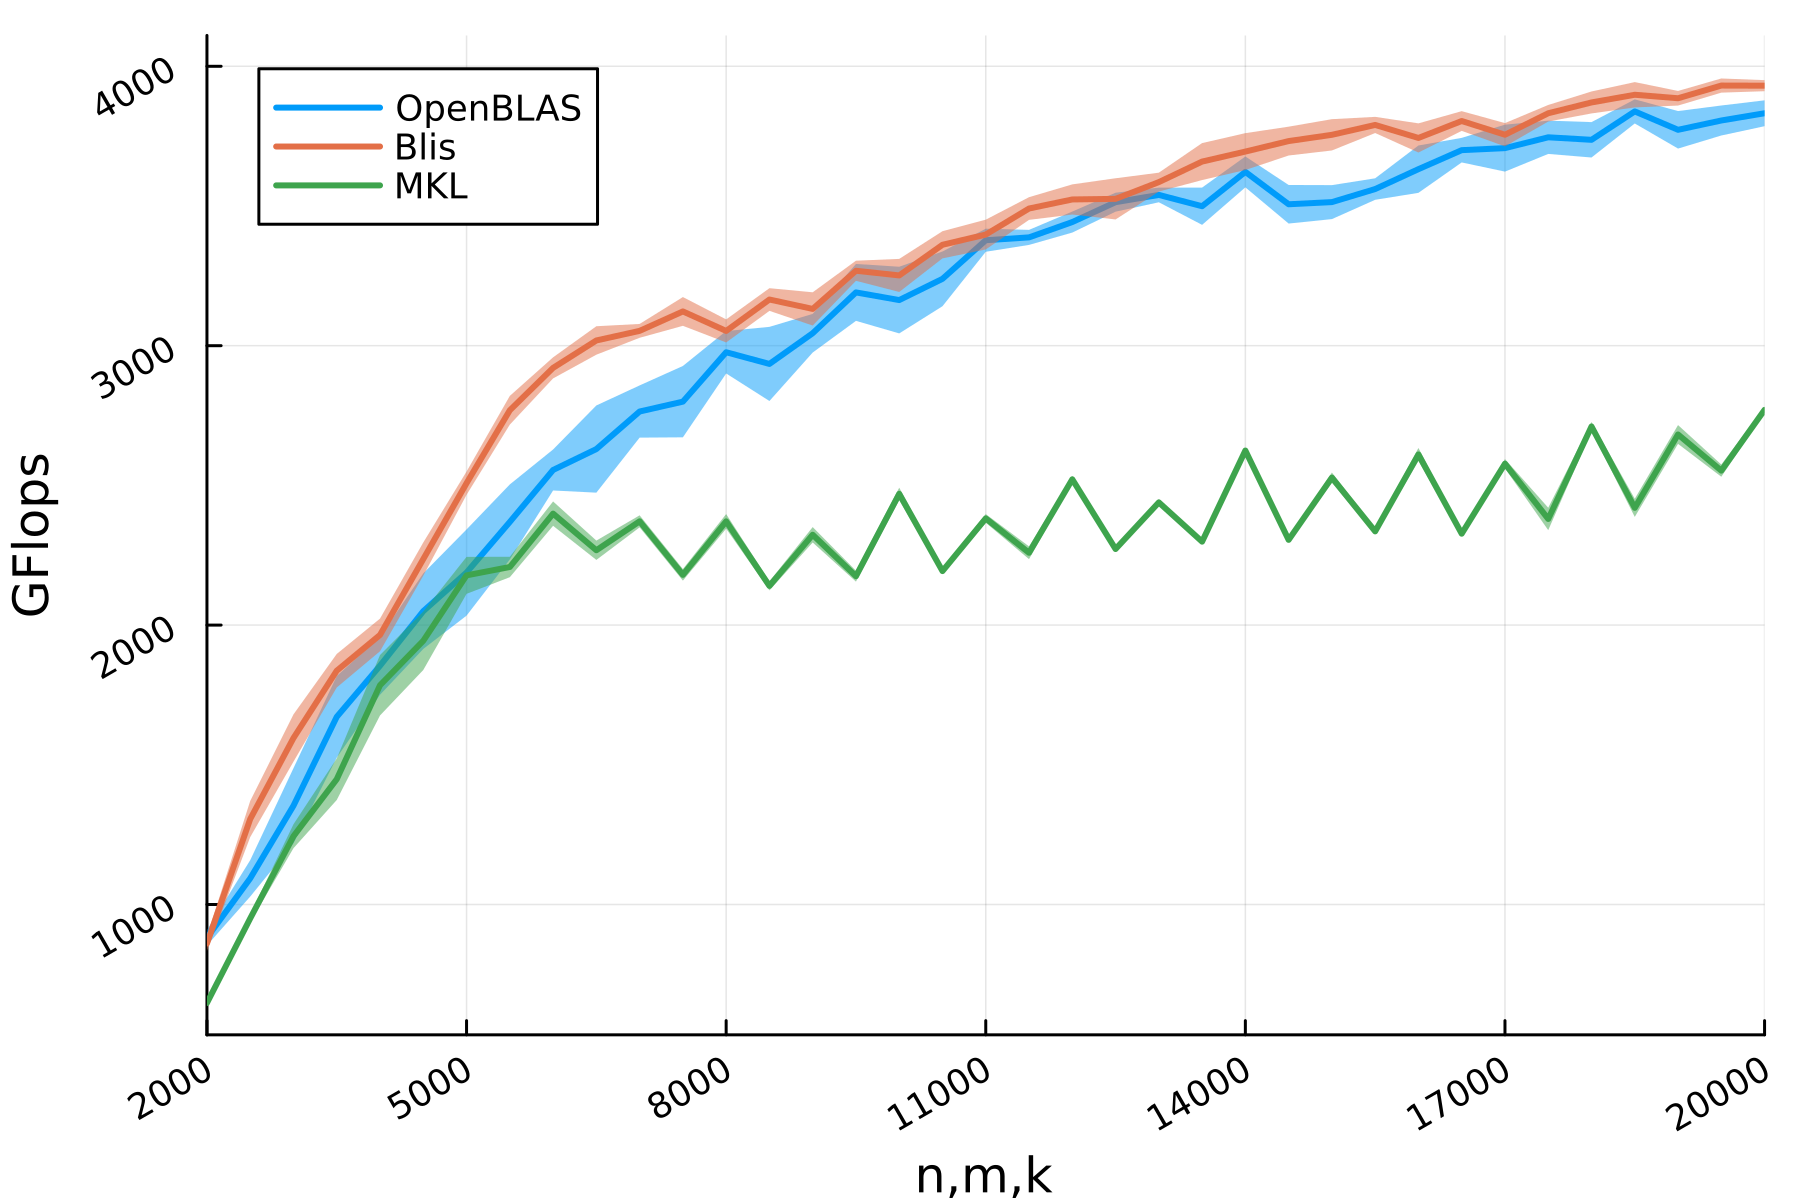
\includegraphics[width=\textwidth,height=3.64583in]{img/float_numactl_close_comparison.png}

}

\caption{Comparison close, with numactl - Float}

\end{figure}

\begin{figure}

{\centering 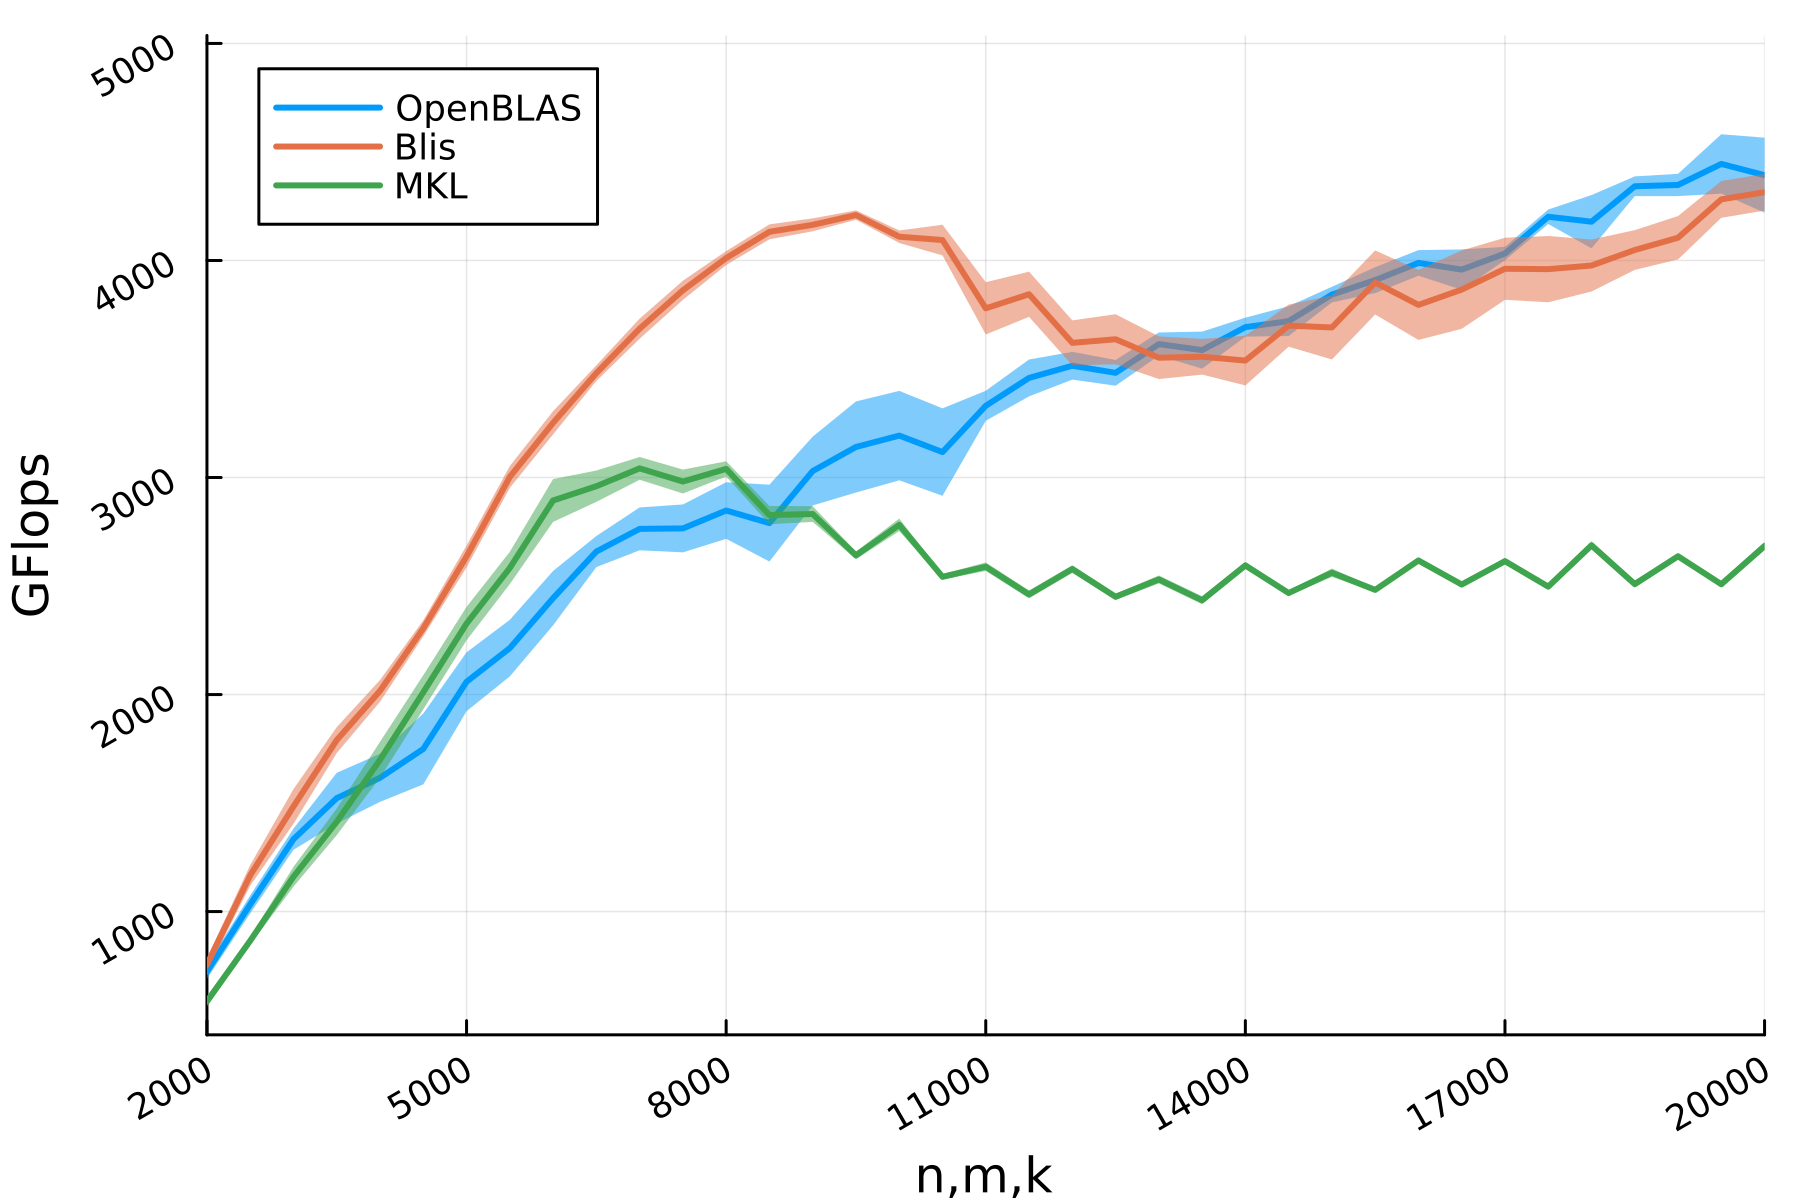
\includegraphics[width=\textwidth,height=3.64583in]{img/float_numactl_spread_comparison.png}

}

\caption{Comparison spread, with numactl - Float}

\end{figure}

\newpage

\hypertarget{double-precision}{%
\subsubsection{Double precision}\label{double-precision}}

The theoretical peak performance for a single socket on an epyc node is:

\[
P = n. cores\cdot frequency \cdot \frac{FLOPC}{cycle} = 64\cdot 2.6 GHz\cdot 16 Flops = 2662.4 GFlops
\]

The table below shows the peak performances:

\begin{longtable}[]{@{}
  >{\raggedright\arraybackslash}p{(\columnwidth - 12\tabcolsep) * \real{0.3725}}
  >{\raggedright\arraybackslash}p{(\columnwidth - 12\tabcolsep) * \real{0.0980}}
  >{\raggedright\arraybackslash}p{(\columnwidth - 12\tabcolsep) * \real{0.1471}}
  >{\raggedright\arraybackslash}p{(\columnwidth - 12\tabcolsep) * \real{0.0882}}
  >{\raggedright\arraybackslash}p{(\columnwidth - 12\tabcolsep) * \real{0.1078}}
  >{\raggedright\arraybackslash}p{(\columnwidth - 12\tabcolsep) * \real{0.0882}}
  >{\raggedright\arraybackslash}p{(\columnwidth - 12\tabcolsep) * \real{0.0980}}@{}}
\toprule()
\begin{minipage}[b]{\linewidth}\raggedright
Settings
\end{minipage} & \begin{minipage}[b]{\linewidth}\raggedright
OpenBlas
\end{minipage} & \begin{minipage}[b]{\linewidth}\raggedright
Size OpenBlas
\end{minipage} & \begin{minipage}[b]{\linewidth}\raggedright
Blis
\end{minipage} & \begin{minipage}[b]{\linewidth}\raggedright
Size Blis
\end{minipage} & \begin{minipage}[b]{\linewidth}\raggedright
MKL
\end{minipage} & \begin{minipage}[b]{\linewidth}\raggedright
Size MKL
\end{minipage} \\
\midrule()
\endhead
close, no numactl & 1134.09 & 16000 & 1168.78 & 16500 & 881.48 &
16000 \\
close, --interleave=0,1,2,3 & 1842.97 & 18500 & 1909.73 & 16500 &
1683.39 & 20000 \\
spread, no numactl & 1225.07 & 17000 & 1222.11 & 17000 & 974.12 &
16500 \\
spread, --interleave=0,1,2,3,4,5,6,7 & 2244.77 & 20000 & 2583.36 & 20000
& 1618.16 & 20000 \\
\bottomrule()
\end{longtable}

The graphs below represent the scaling of math library when the policy
changes (one graph for each policy).

From the OpenBLAS plot we can see that the usage of numactl improves the
performance. If we look at \texttt{OMP\_PROC\_BIND=close} and
\texttt{OMP\_PROC\_BIND=spread} both with the usage of numactl we can
understand that until \(n=m=k=15000\) they are almost equivalent. After
that \texttt{OMP\_PROC\_BIND=spread} overcame
\texttt{OMP\_PROC\_BIND=close} if we consider the curves with numactl.

The Blis graph shows that \texttt{OMP\_PROC\_BIND=spread} with the usage
of numactl is the best policy almost everywhere. It is important to
highlight that there is a large drop in performance at \(n=m=k=11000\)
for all the policies.

As it concern MKL we can se that the policy
\texttt{OMP\_PROC\_BIND=spread} with the usage of numactl performs
better in the initial part and, after a peak at \(n=m=k=10000\), it has
a drop in performances. On the tail the policy
\texttt{OMP\_PROC\_BIND=close} with numactl works better then the
others.

\begin{figure}

{\centering 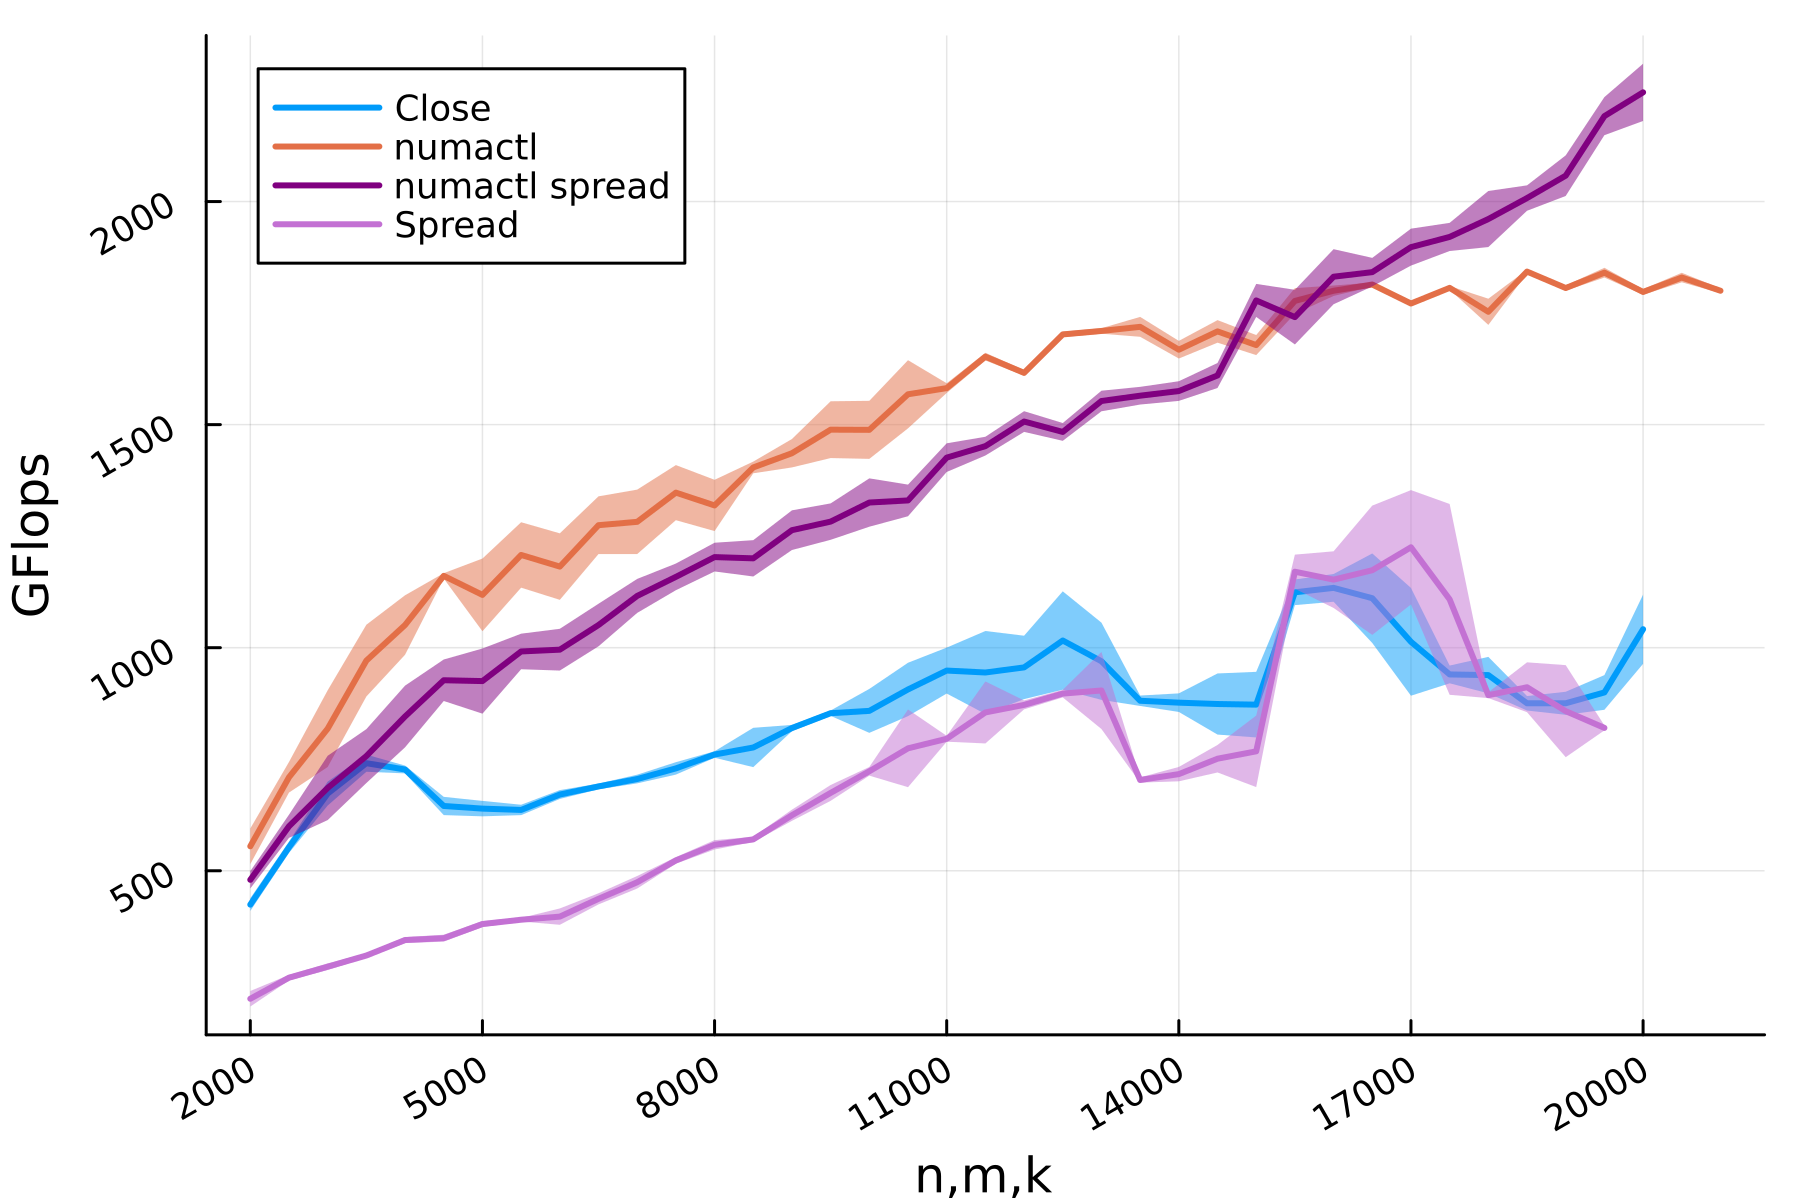
\includegraphics[width=\textwidth,height=3.64583in]{img/double_obblas_comparison.png}

}

\caption{Comparison OpenBlas - Double}

\end{figure}

\begin{figure}

{\centering 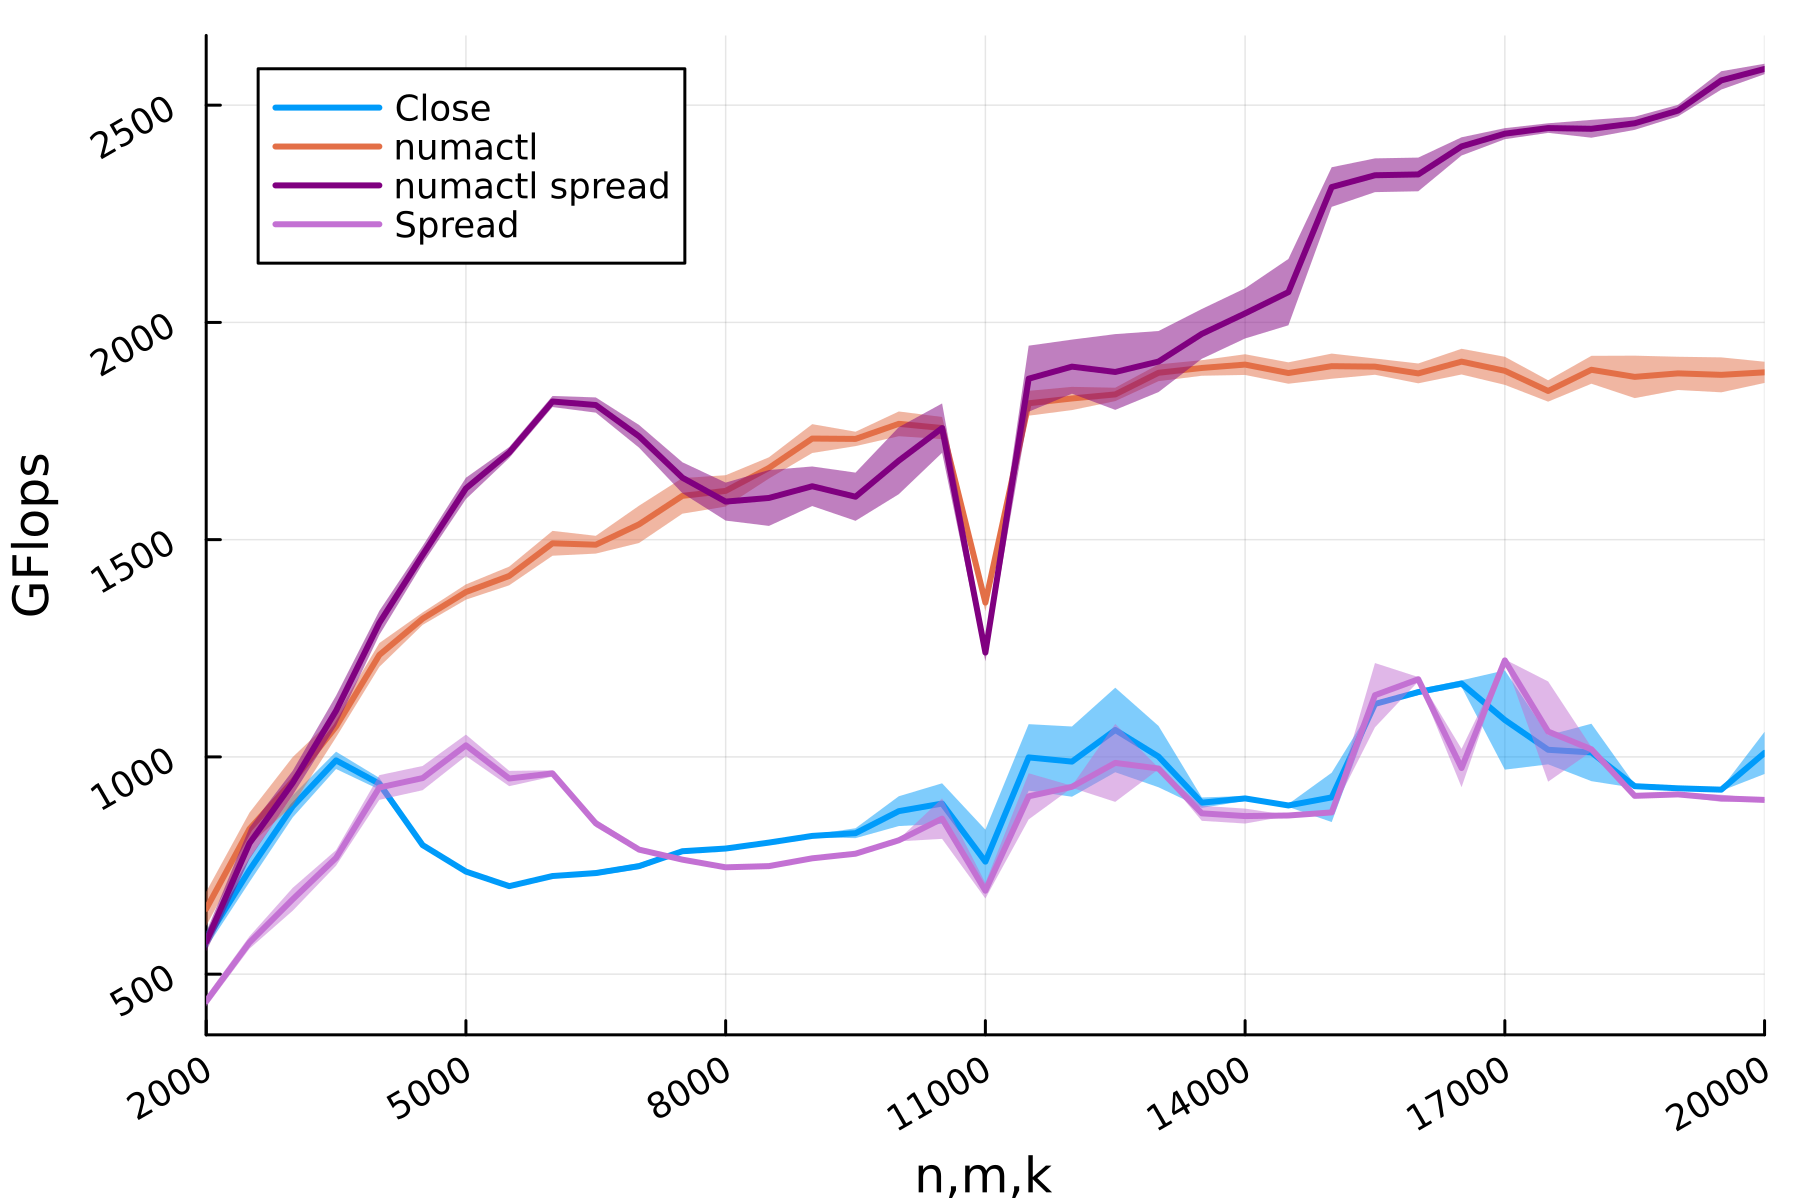
\includegraphics[width=\textwidth,height=3.64583in]{img/double_blis_comparison.png}

}

\caption{Comparison Blis - Double}

\end{figure}

\begin{figure}

{\centering 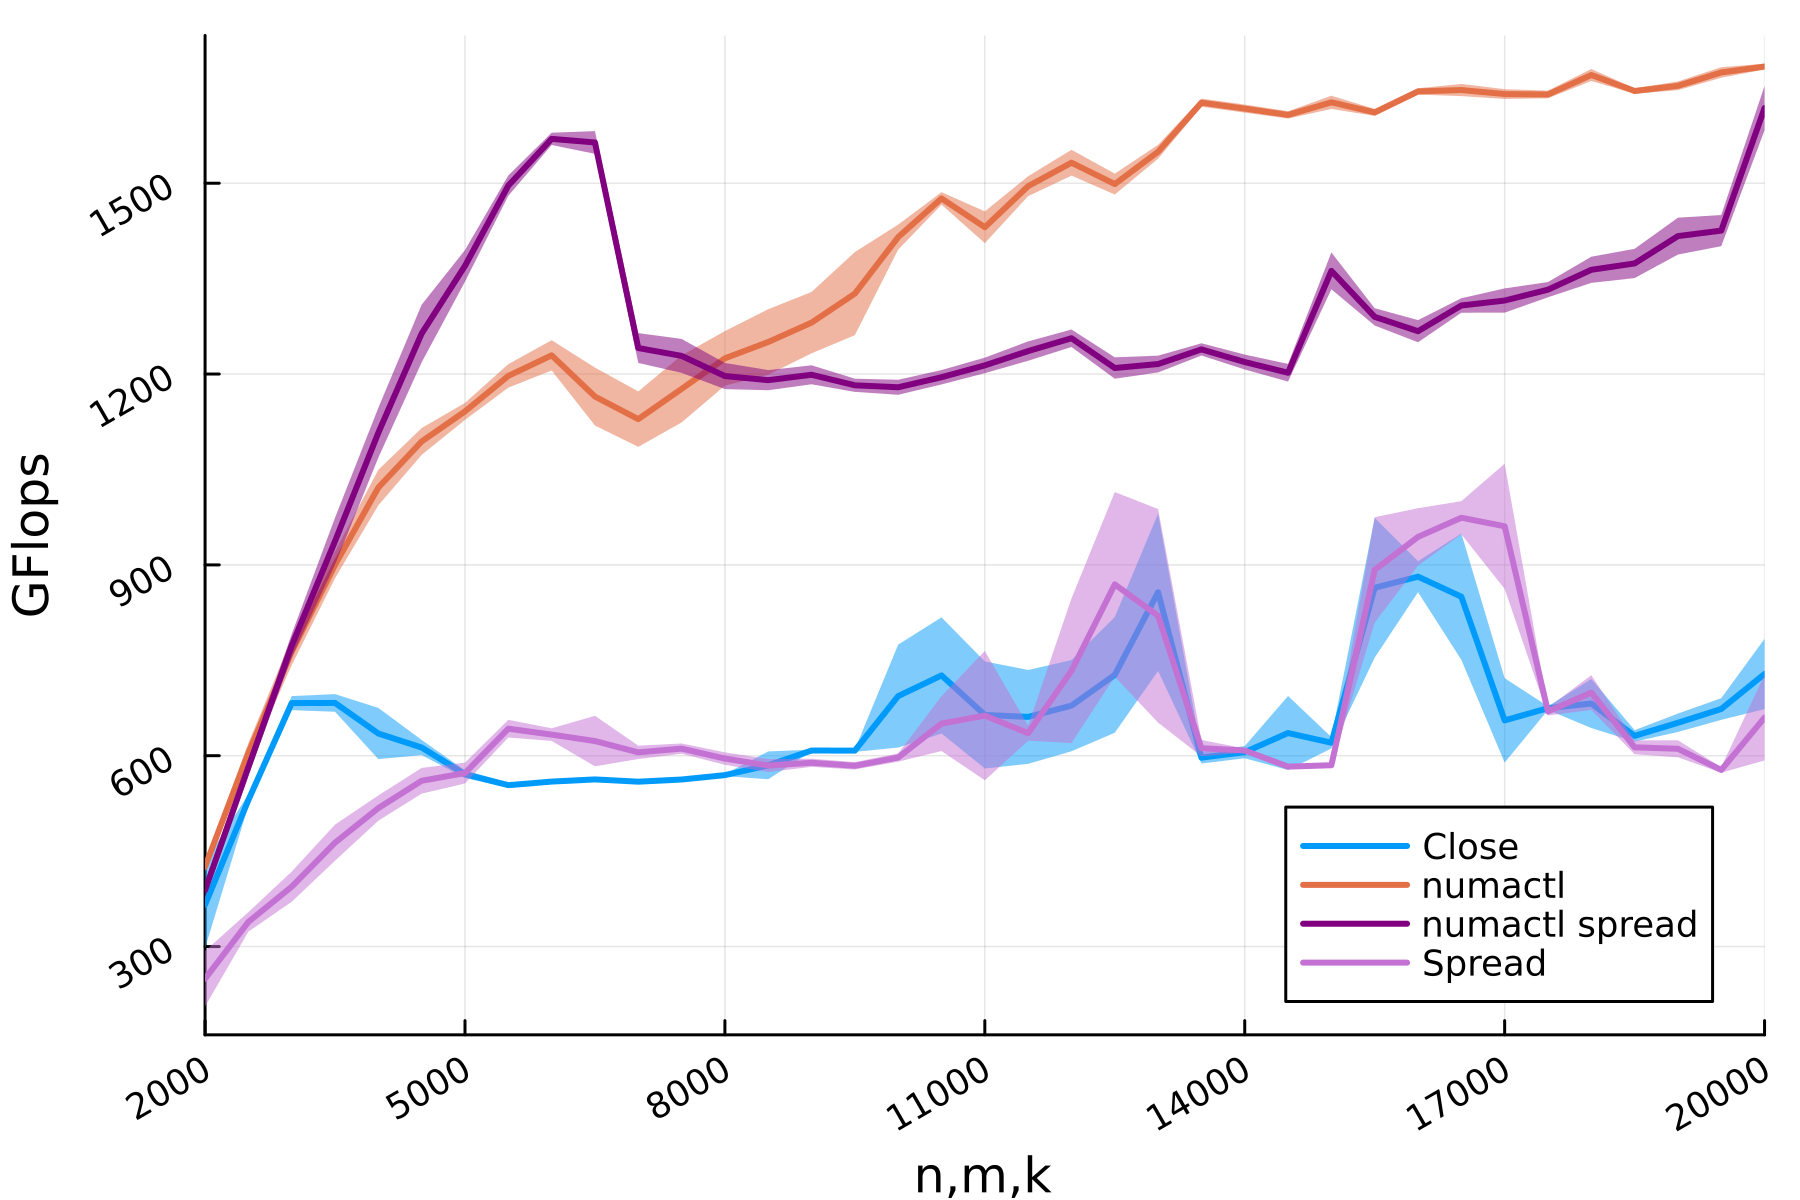
\includegraphics[width=\textwidth,height=3.64583in]{img/double_mkl_comparison.png}

}

\caption{Comparison MKL - Double}

\end{figure}

\newpage

In the graphs below I have gathered togheter the different math
libraries (one plot for each policy).

If we look the graph of the policy \texttt{OMP\_PROC\_BIND=close} with
the usage of numactl we can see that the best math library is Blis
followed by OpenBlas. The worst one is MKL. All the three lines follows
almost the same trend

In the end, the graph of the policy \texttt{OMP\_PROC\_BIND=spread} with
the usage of numactl show us that the best library is Blis followed by
openBlas and MKL. In this case the peak performance of the best library
(Blis) is 2244.77, much larger than the peak performance in the other
cases.

\begin{figure}

{\centering 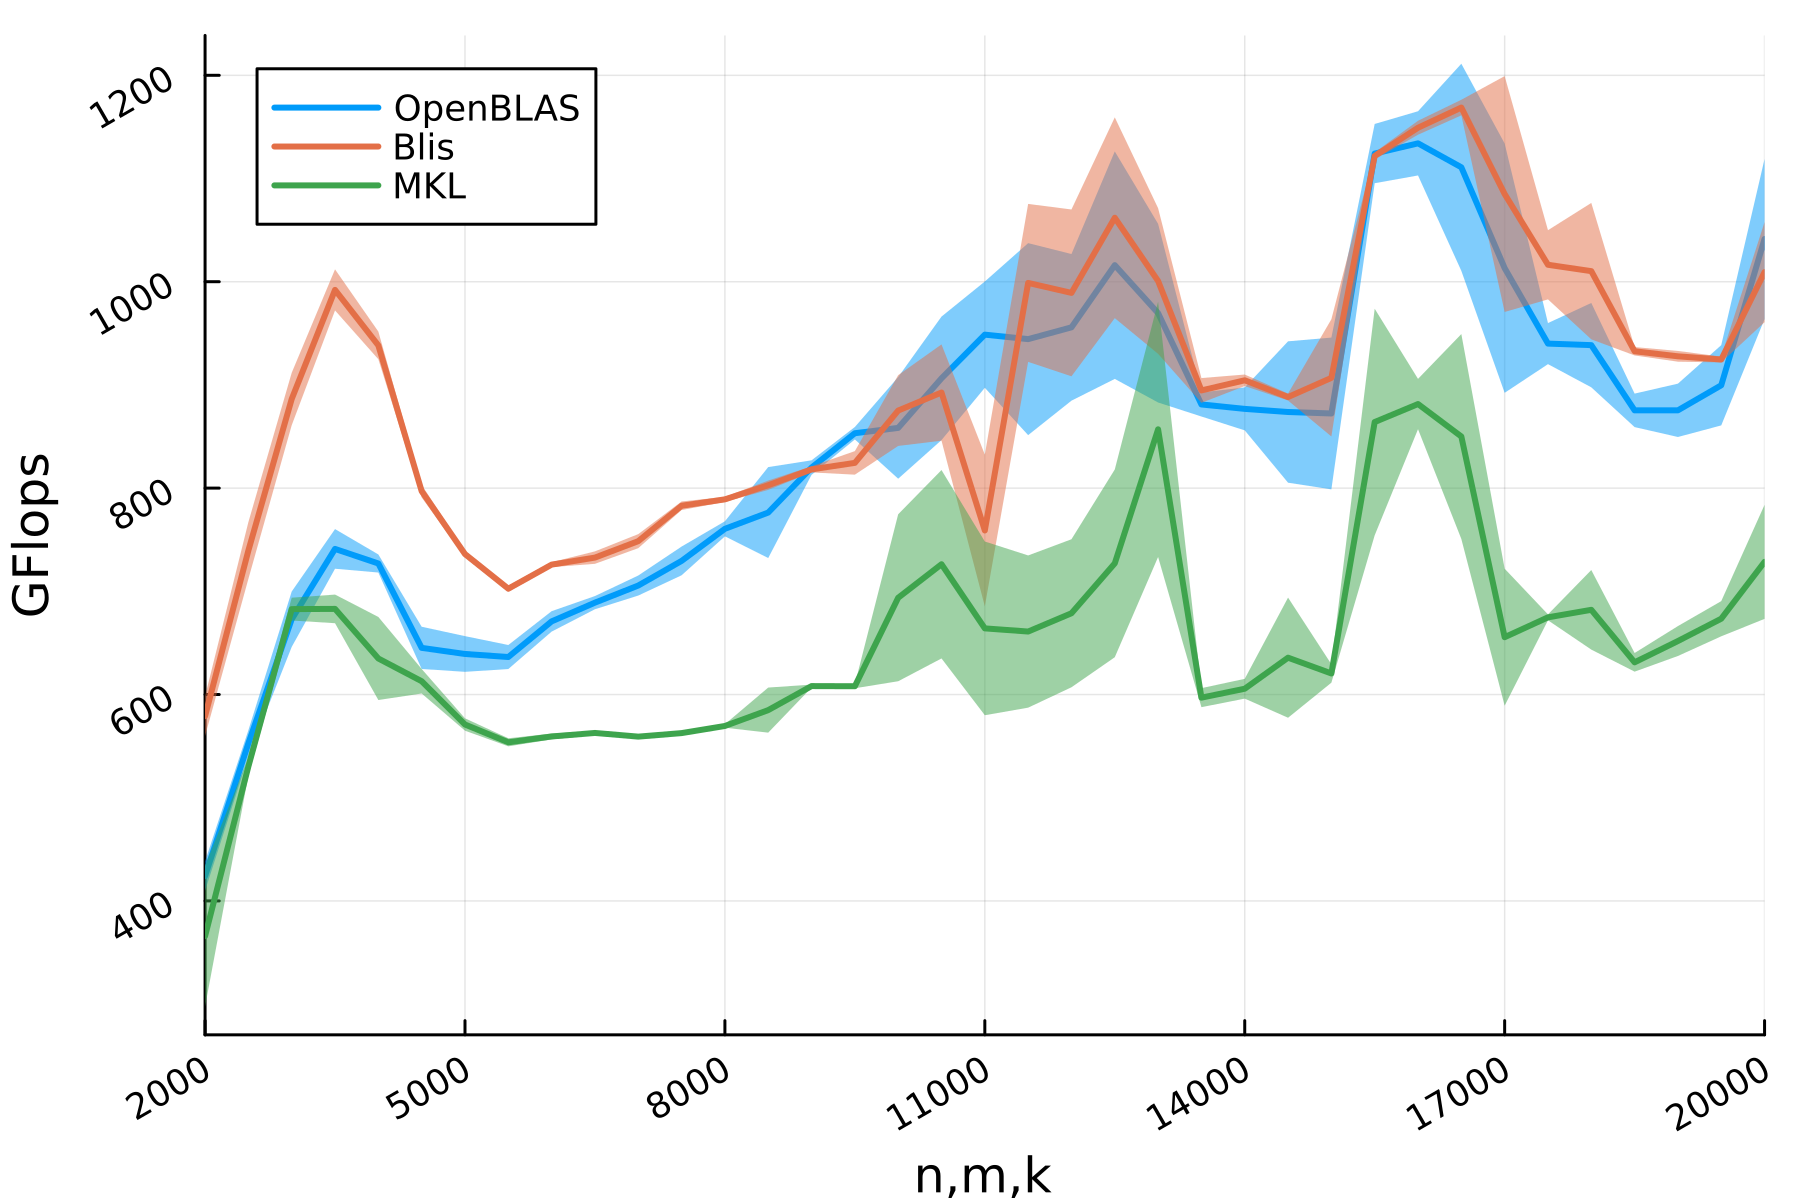
\includegraphics[width=\textwidth,height=3.64583in]{img/double_close_comparison.png}

}

\caption{Comparison close, no numactl options - Double}

\end{figure}

\begin{figure}

{\centering 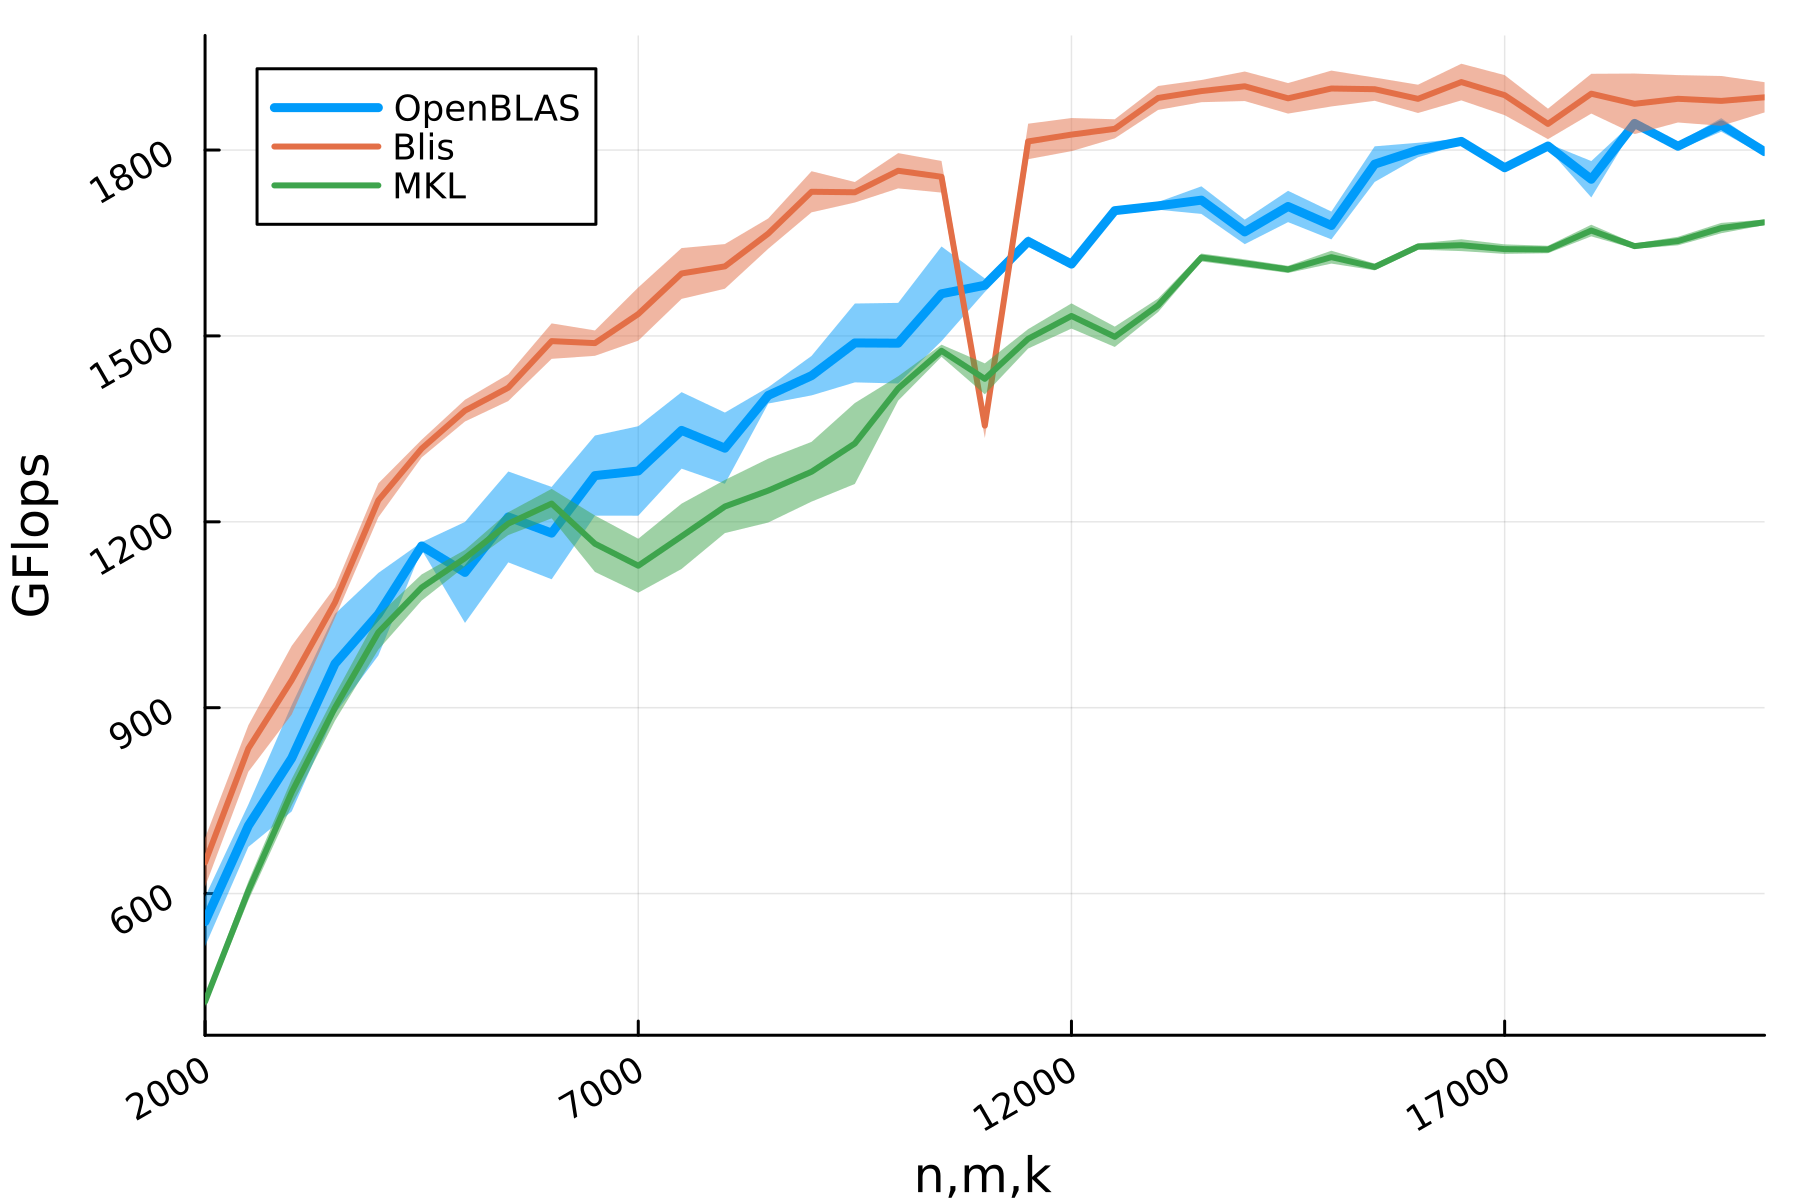
\includegraphics[width=\textwidth,height=3.64583in]{img/double_numactl_close_comparison.png}

}

\caption{Comparison close, with numactl - Double}

\end{figure}

\begin{figure}

{\centering 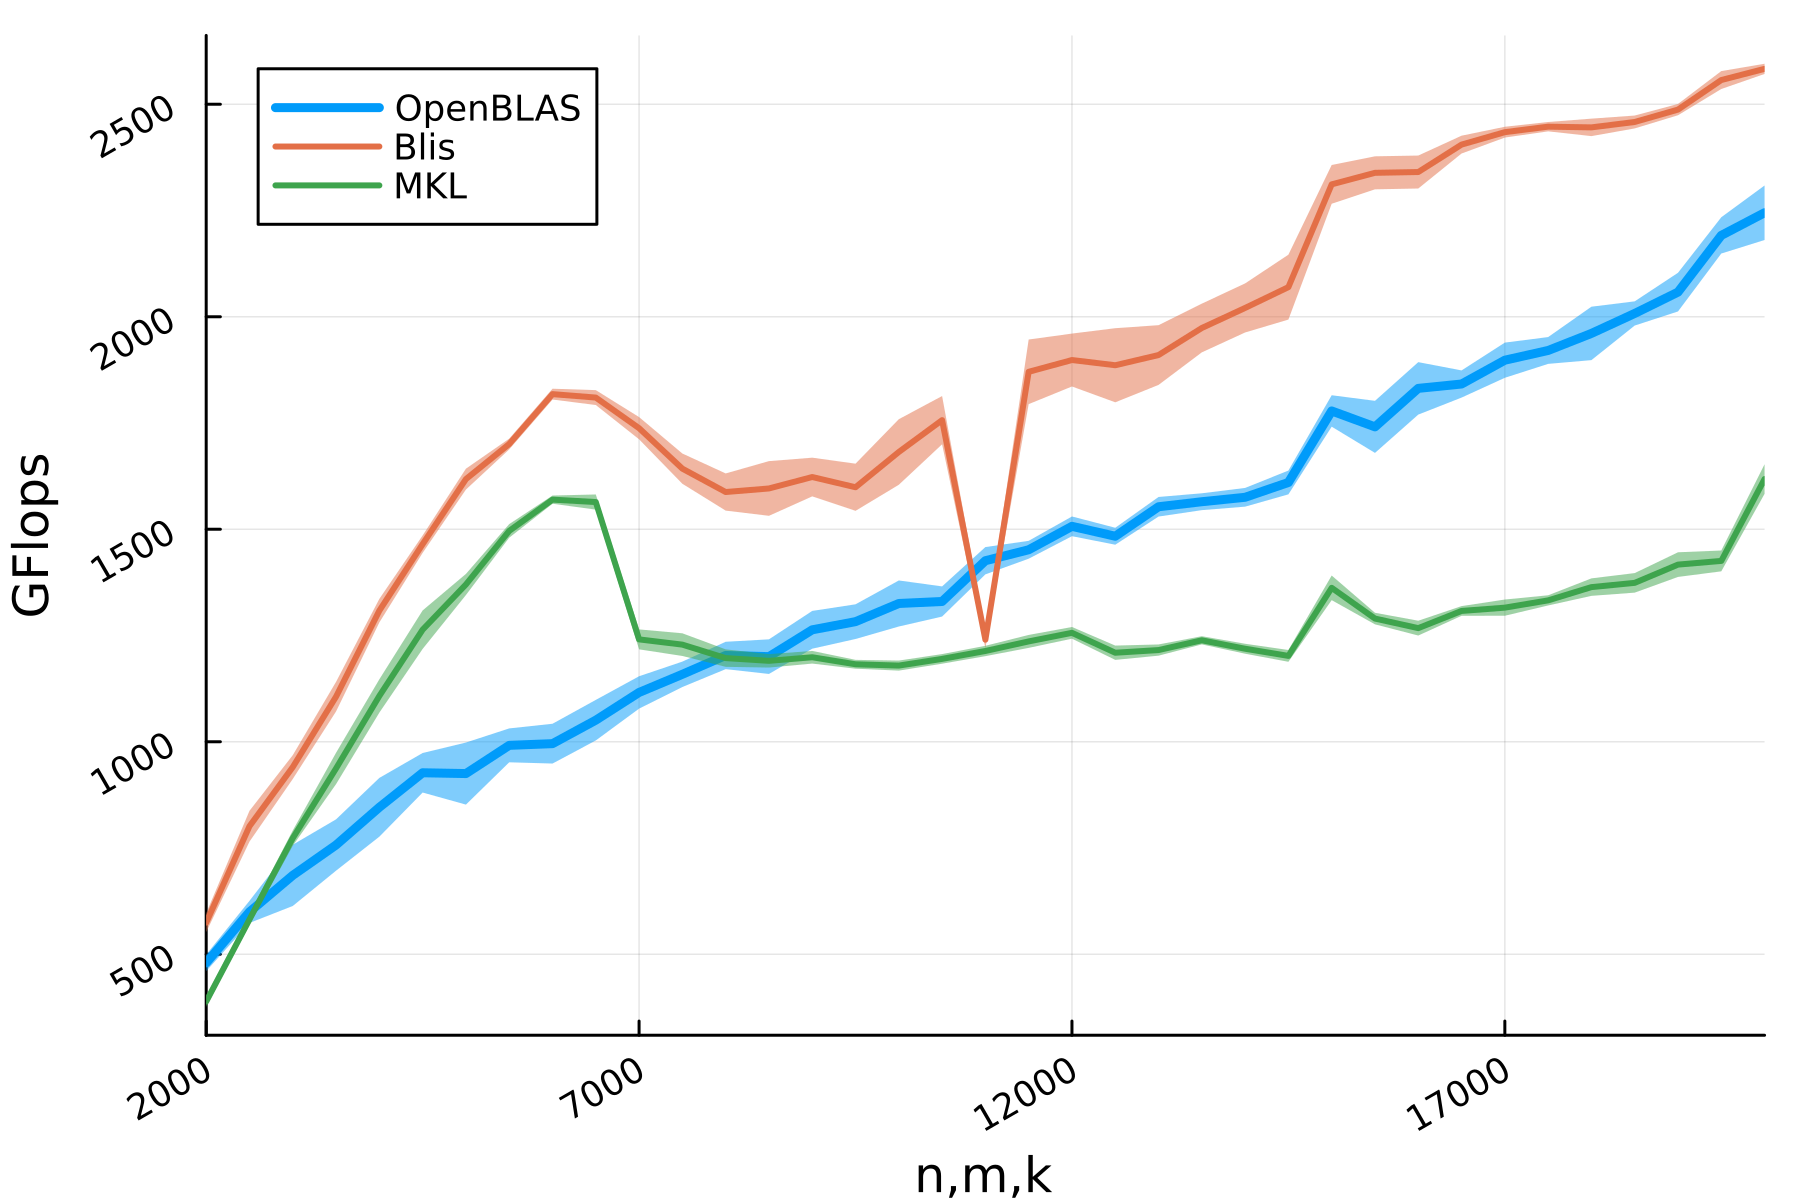
\includegraphics[width=\textwidth,height=3.64583in]{img/double_numactl_spread_comparison.png}

}

\caption{Comparison spread, with numactl - Double}

\end{figure}

\newpage

\hypertarget{core-scaling}{%
\subsection{Core scaling}\label{core-scaling}}

In this section I analyze the behaviour of the different math libraries
on a fixed value of \(n,m,k\) when the number of OpenMP threads
increases. I have run the program for two different values of the
parameter, \(10000\) and \(20000\). The policy that I have tested are:

\begin{itemize}
\tightlist
\item
  \texttt{OMP\_PROC\_BIND=close} whitout numactl options
\item
  \texttt{OMP\_PROC\_BIND=close} with the following numaclt policy:

  \begin{itemize}
  \tightlist
  \item
    From 1 to 16 OpenMP threads: \texttt{-\/-interleave=0}
  \item
    From 17 to 32 OpenMP threads: \texttt{-\/-interleave=0,1}
  \item
    From 33 to 48 OpenMP threads: \texttt{-\/-interleave=0,1,2}
  \item
    From 49 to 64 OpenMP threads: \texttt{-\/-interleave=0,1,2,3}
  \end{itemize}
\item
  \texttt{OMP\_PROC\_BIND=spread} without numaclt policy:
\end{itemize}

\hypertarget{single-precision}{%
\subsubsection{Single precision}\label{single-precision}}

The plots below show the OpenMP scalability. In all the three cases we
have the maximum scalability when we use the policy
\texttt{OMP\_PROC\_BIND=close} and numactl. The graphs of Blis and MKL
when \(n=m=k=10000\) shows that the speed up with
\texttt{OMP\_PROC\_BIND=spread} has a strange behavious on the right
tail.

\begin{figure}

{\centering 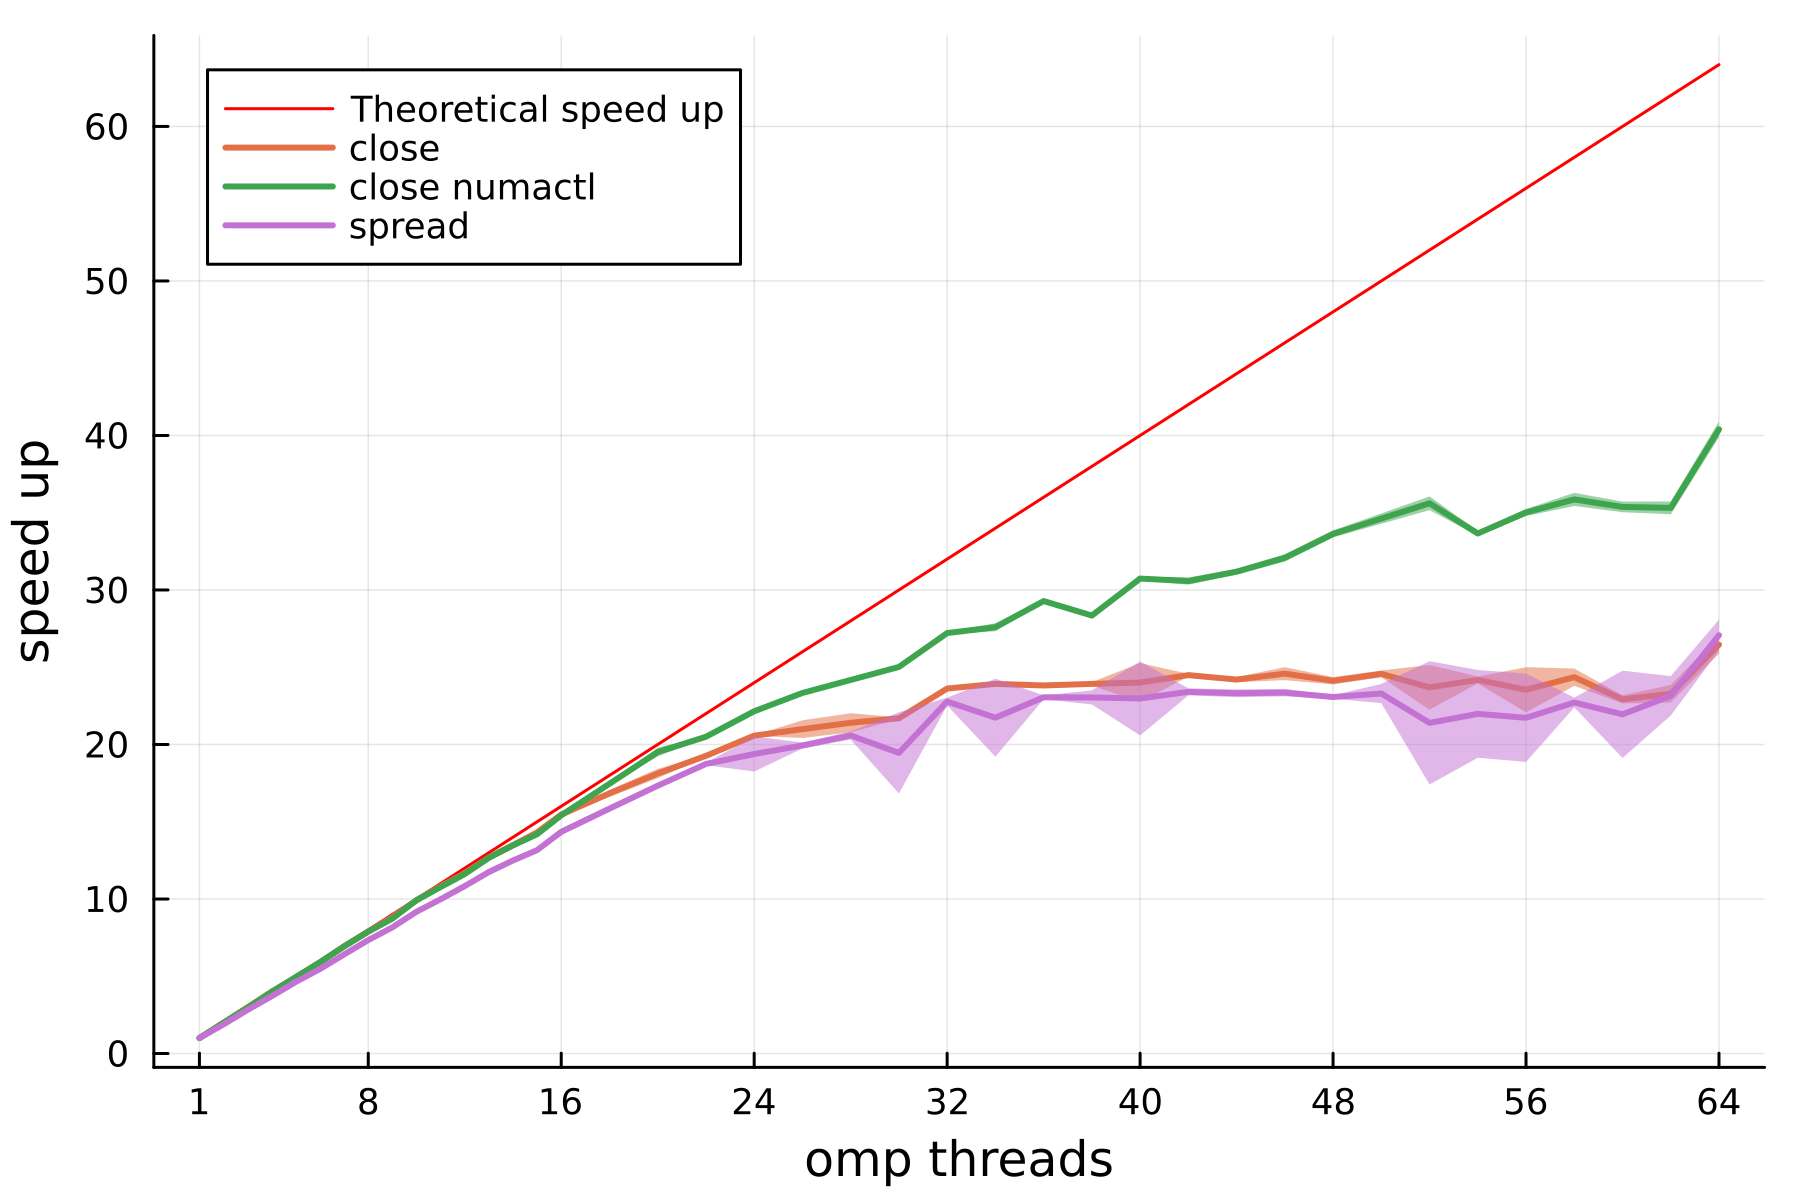
\includegraphics[width=\textwidth,height=3.64583in]{img/oblas_scalability_20000.png}

}

\caption{OpenBlas scalability, n=m=k=20000 - Float}

\end{figure}

\begin{figure}

{\centering 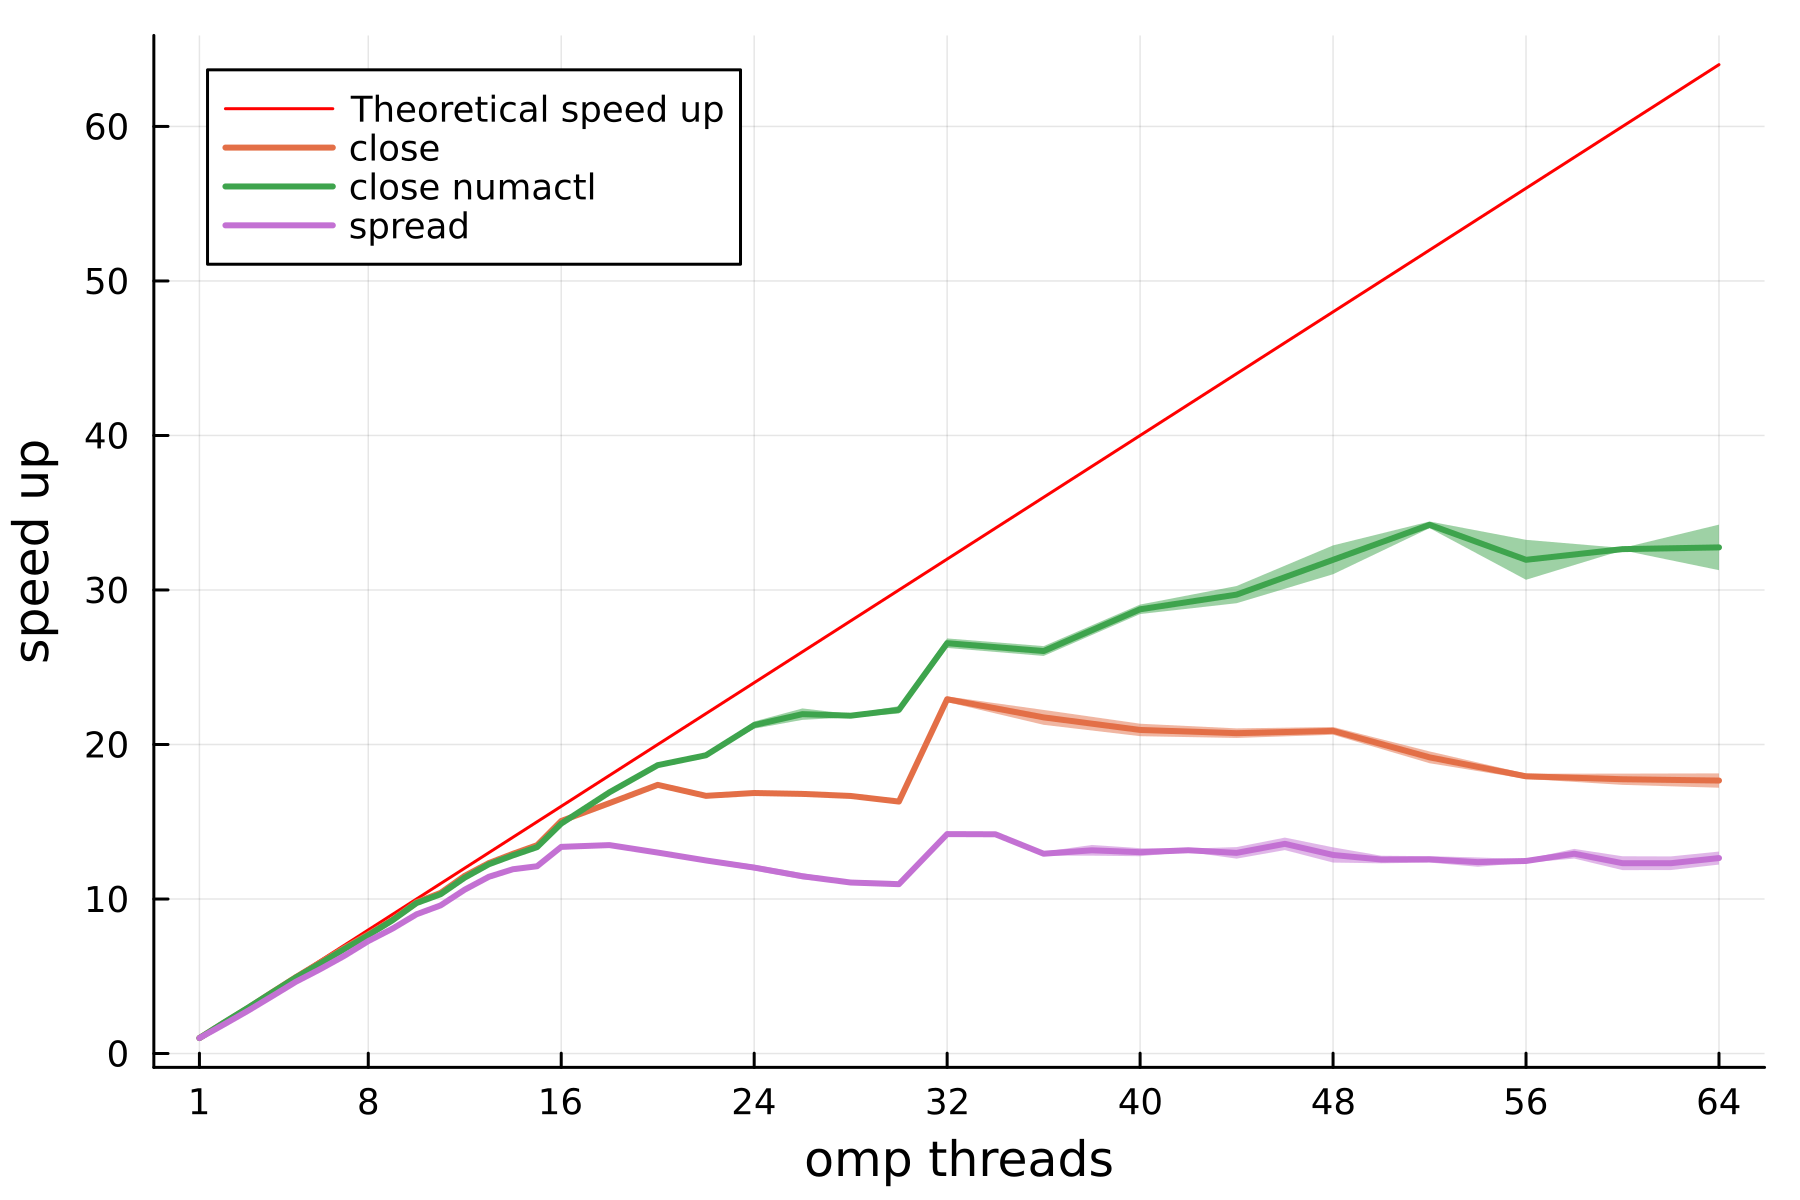
\includegraphics[width=\textwidth,height=3.64583in]{img/oblas_scalability_10000.png}

}

\caption{OpenBlas scalability, n=m=k=10000 - Float}

\end{figure}

\begin{figure}

{\centering 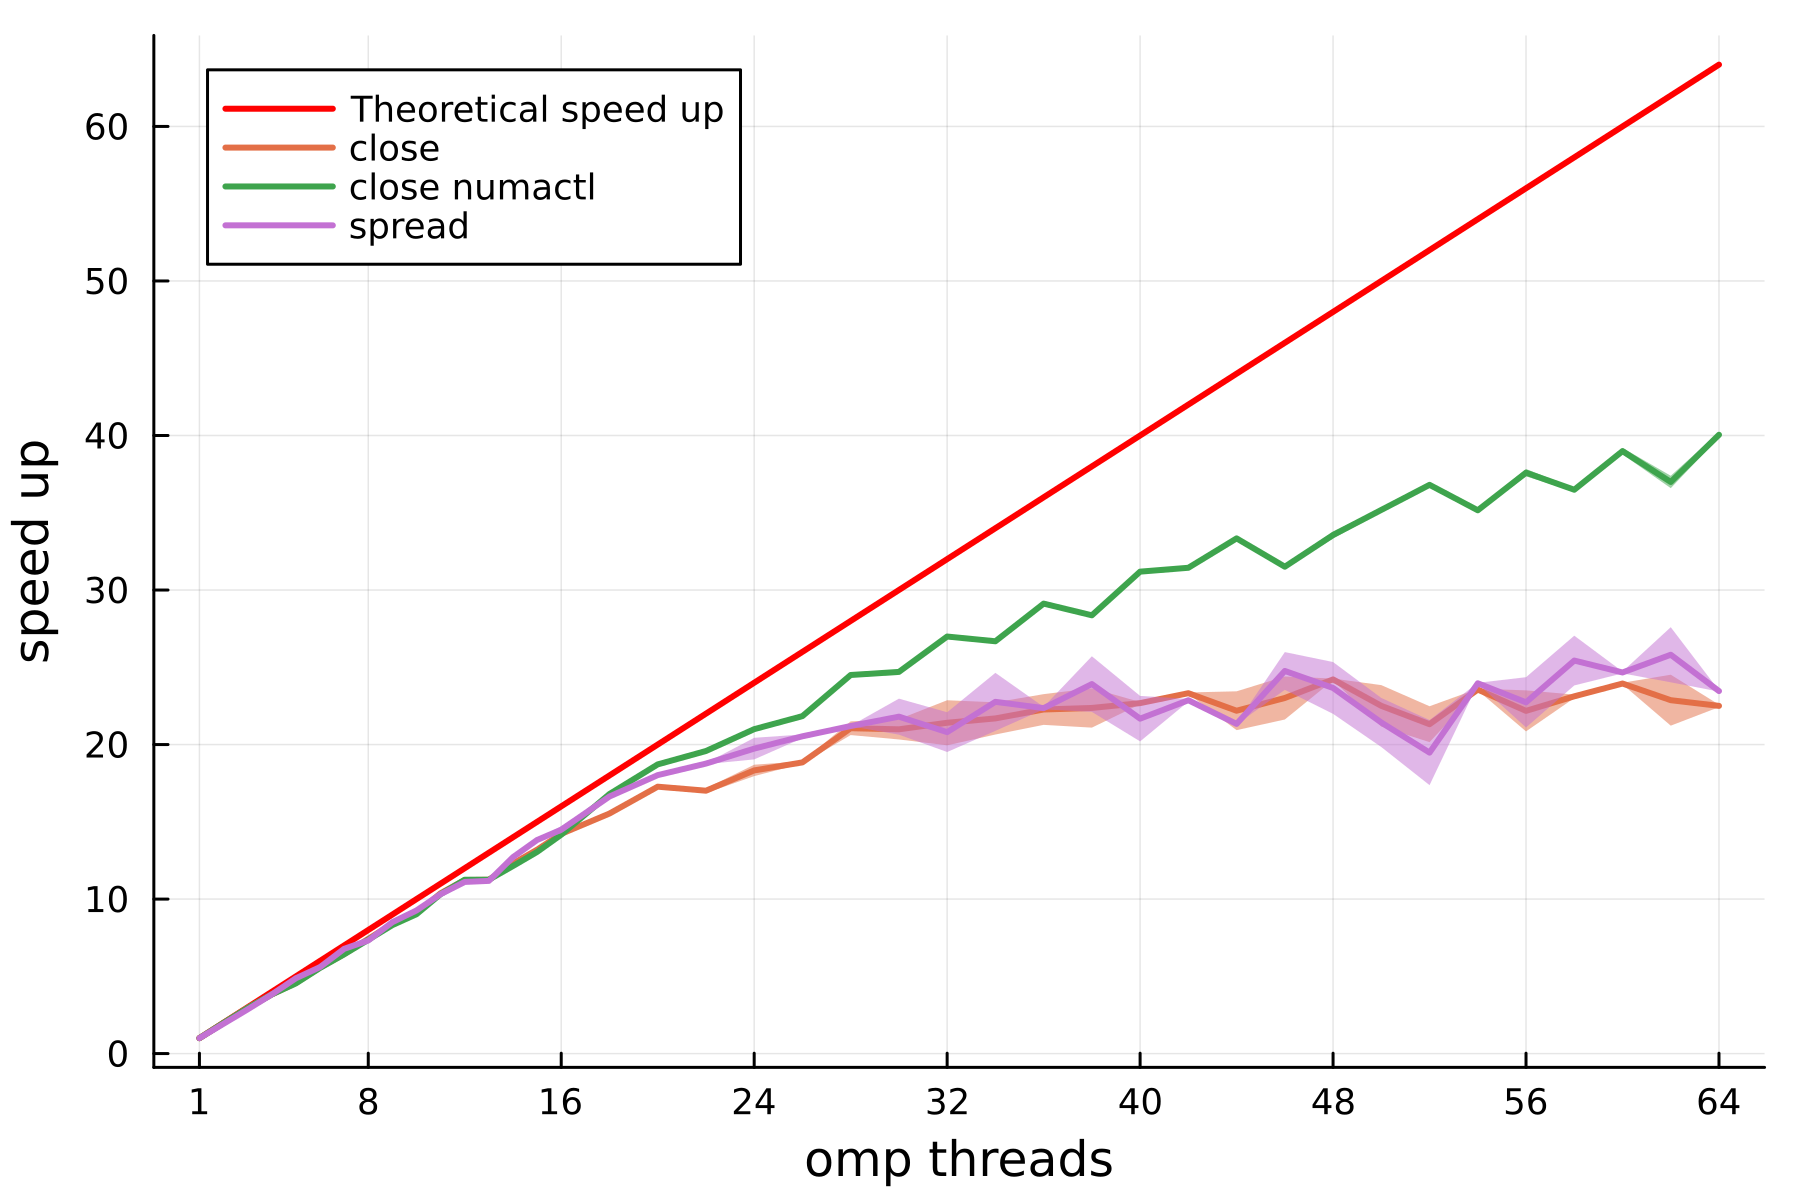
\includegraphics[width=\textwidth,height=3.64583in]{img/blis_scalability_20000.png}

}

\caption{Blis scalability, n=m=k=20000 - Float}

\end{figure}

\begin{figure}

{\centering 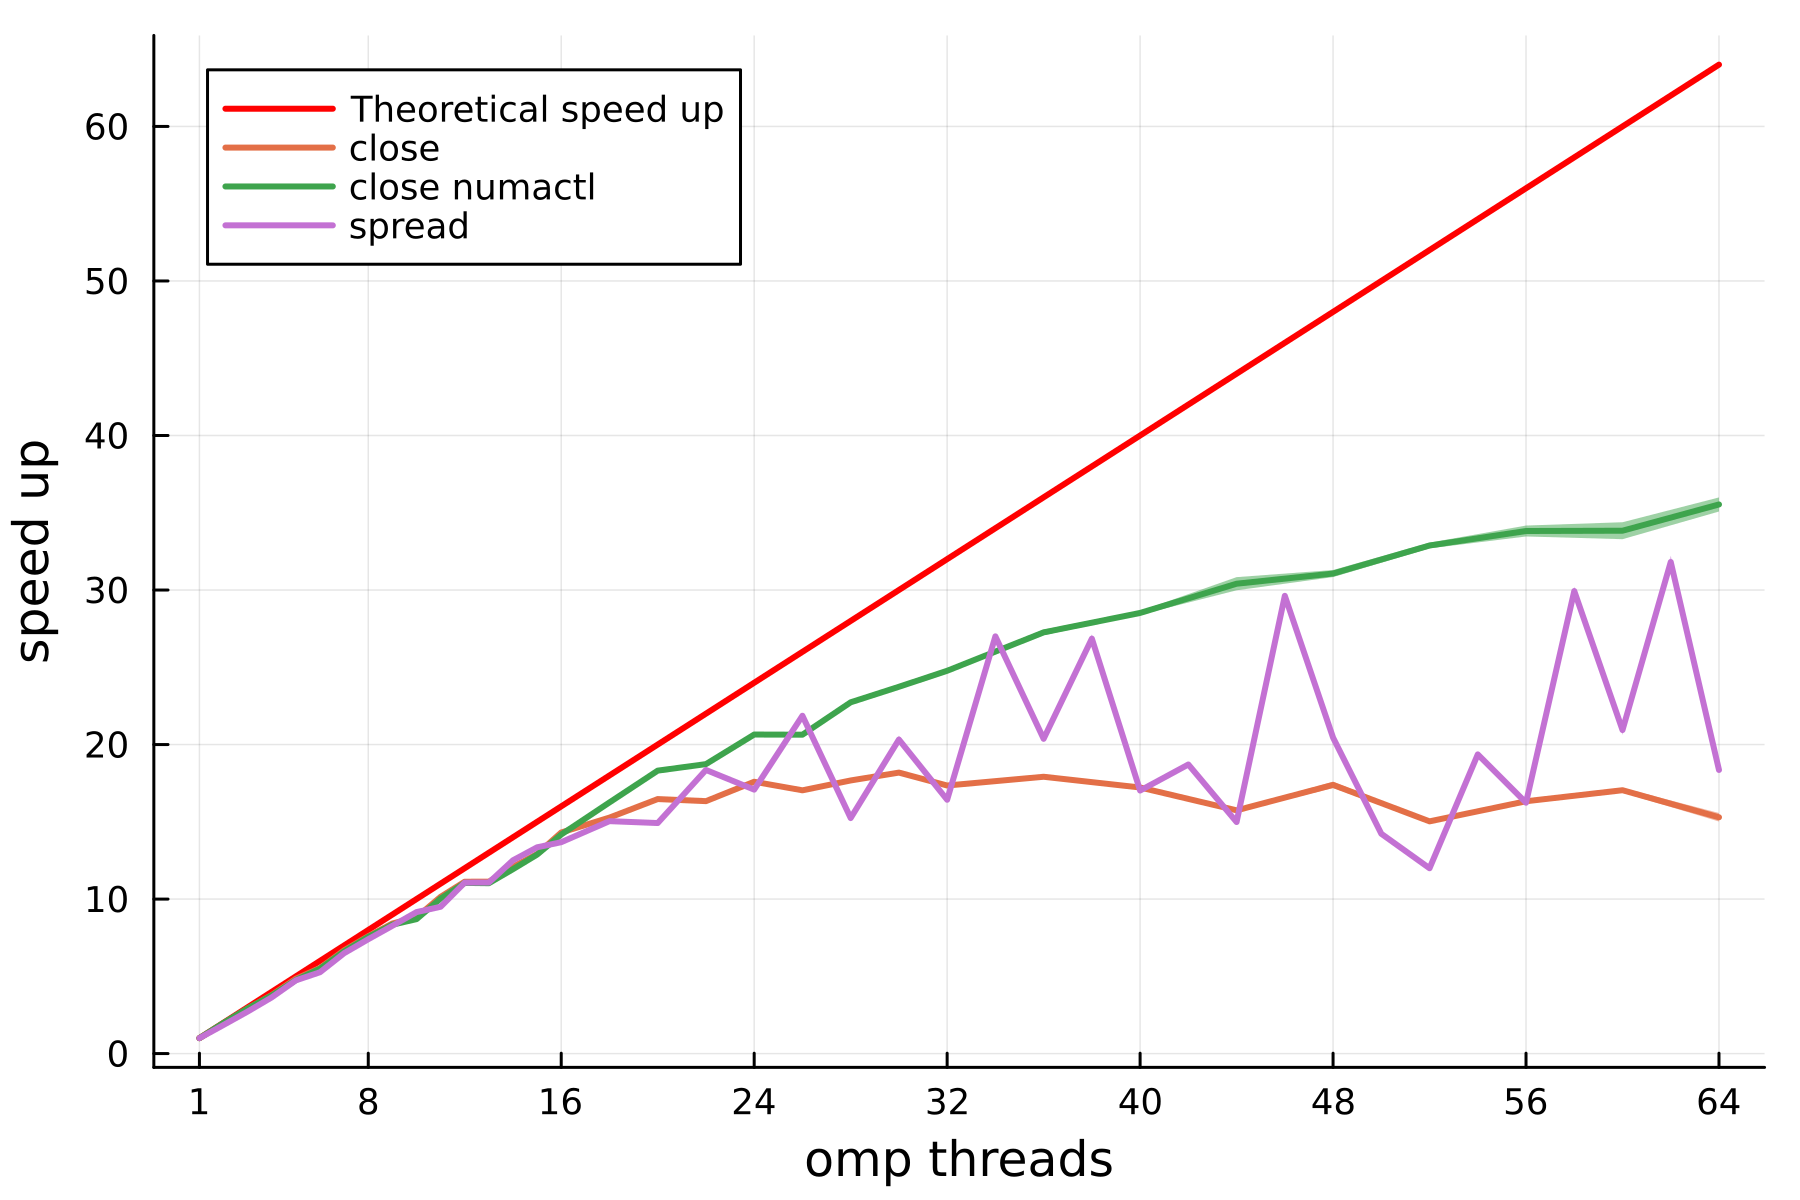
\includegraphics[width=\textwidth,height=3.64583in]{img/blis_scalability_10000.png}

}

\caption{Blis scalability, n=m=k=10000 - Float}

\end{figure}

\begin{figure}

{\centering 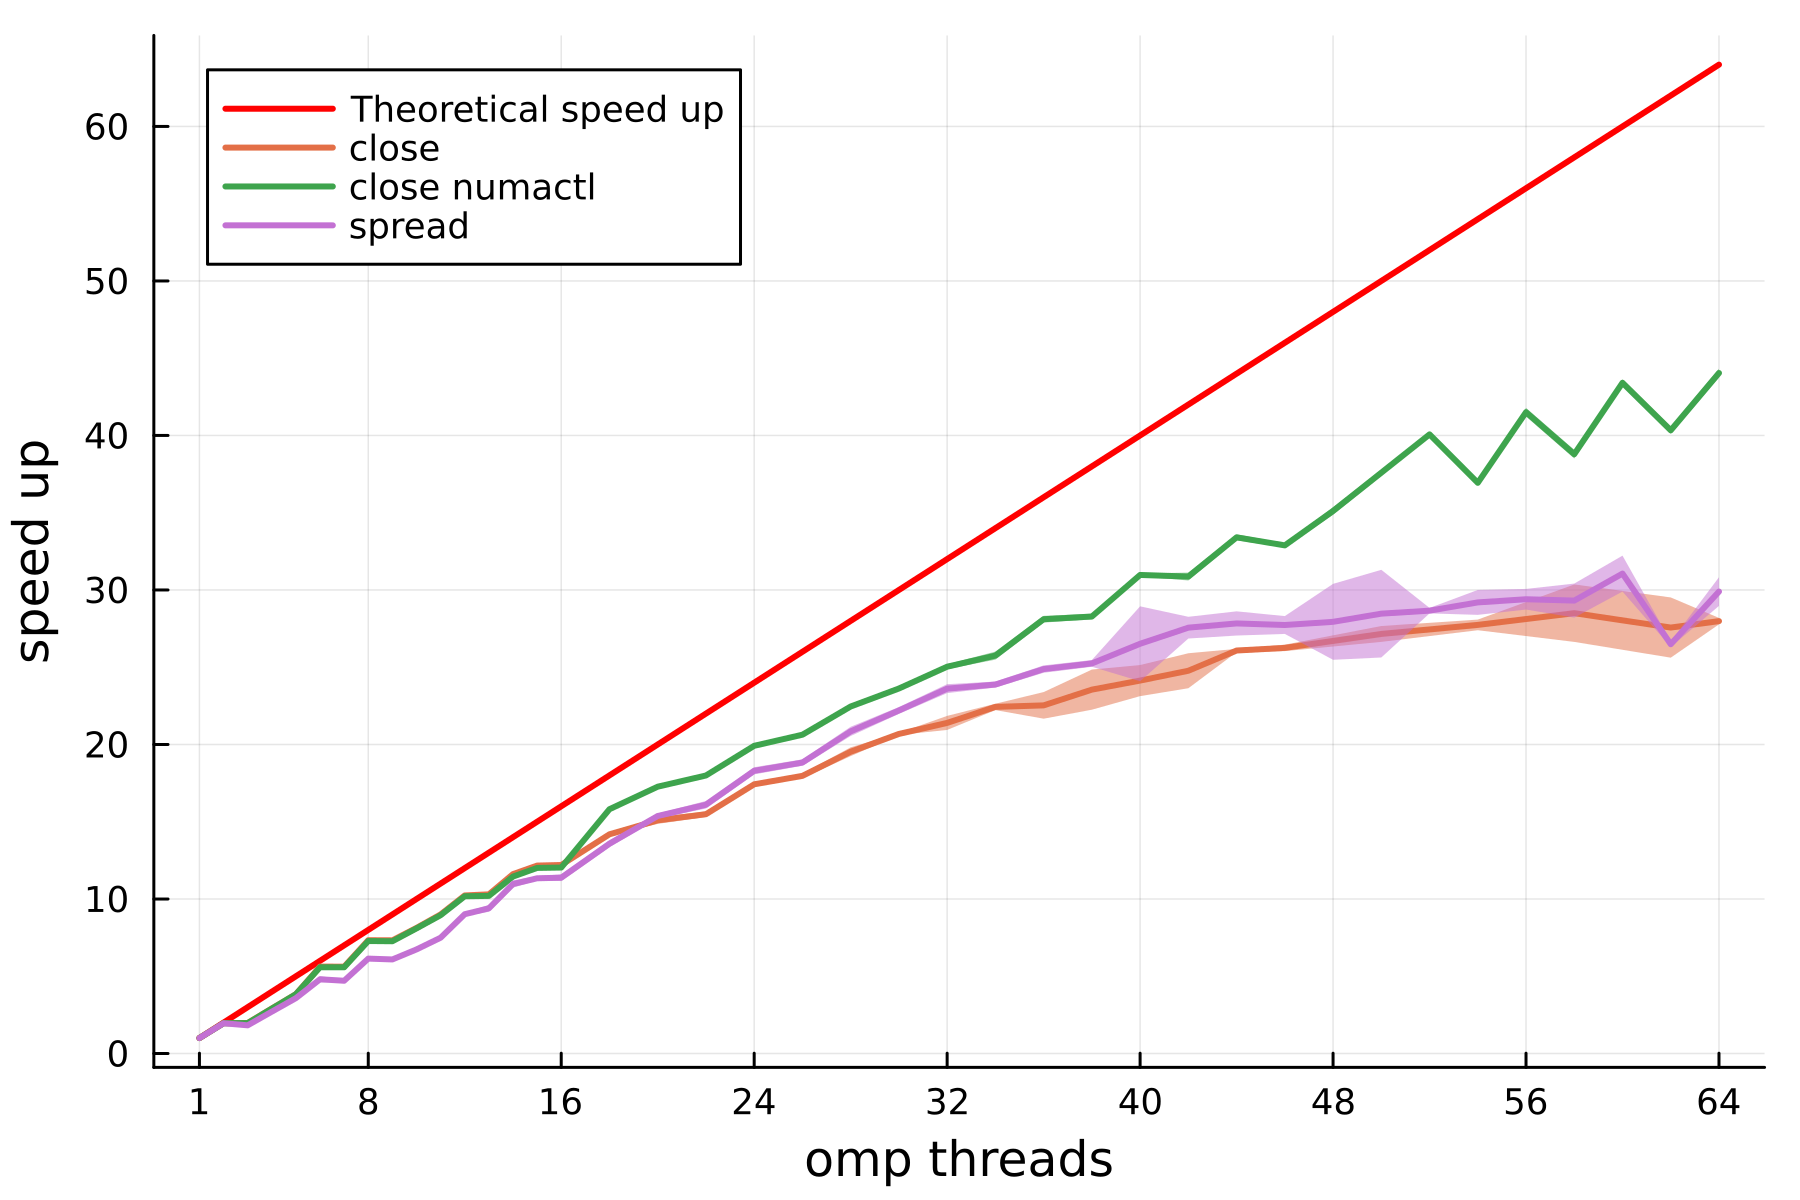
\includegraphics[width=\textwidth,height=3.64583in]{img/mkl_scalability_20000.png}

}

\caption{MKL scalability, n=m=k=20000 - Float}

\end{figure}

\begin{figure}

{\centering 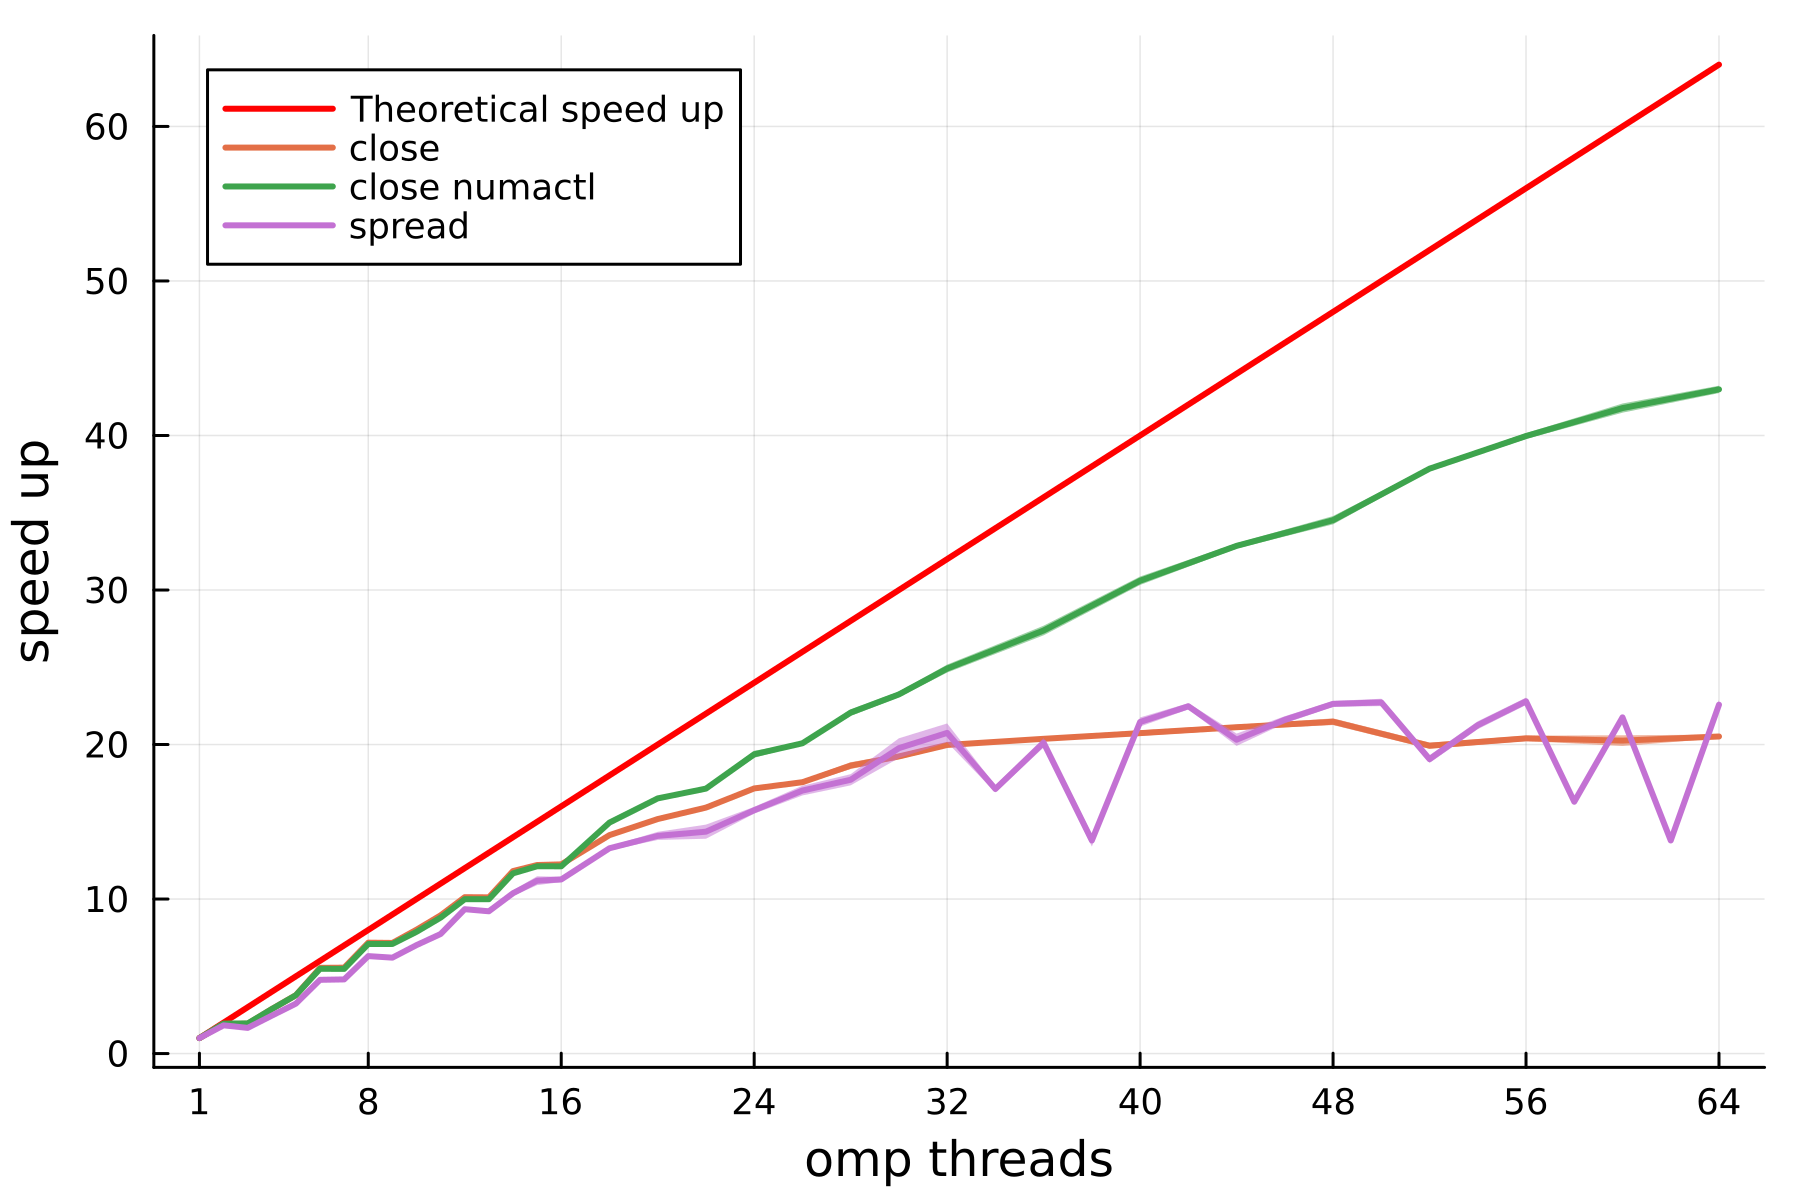
\includegraphics[width=\textwidth,height=3.64583in]{img/mkl_scalability_10000.png}

}

\caption{MKL scalability, n=m=k=10000 - Float}

\end{figure}

\newpage

\hypertarget{double-precision-1}{%
\subsubsection{Double precision}\label{double-precision-1}}

The plots below show the OpenMP scalability. In all the three cases we
have the maximum scalability when we use the policy
\texttt{OMP\_PROC\_BIND=close} and numactl. We can notice, also in this
case, a strage behaviour of the speed up for Blis with
\texttt{OMP\_PROC\_BIND=spread} and \(n=m=k=10000\).

\begin{figure}

{\centering 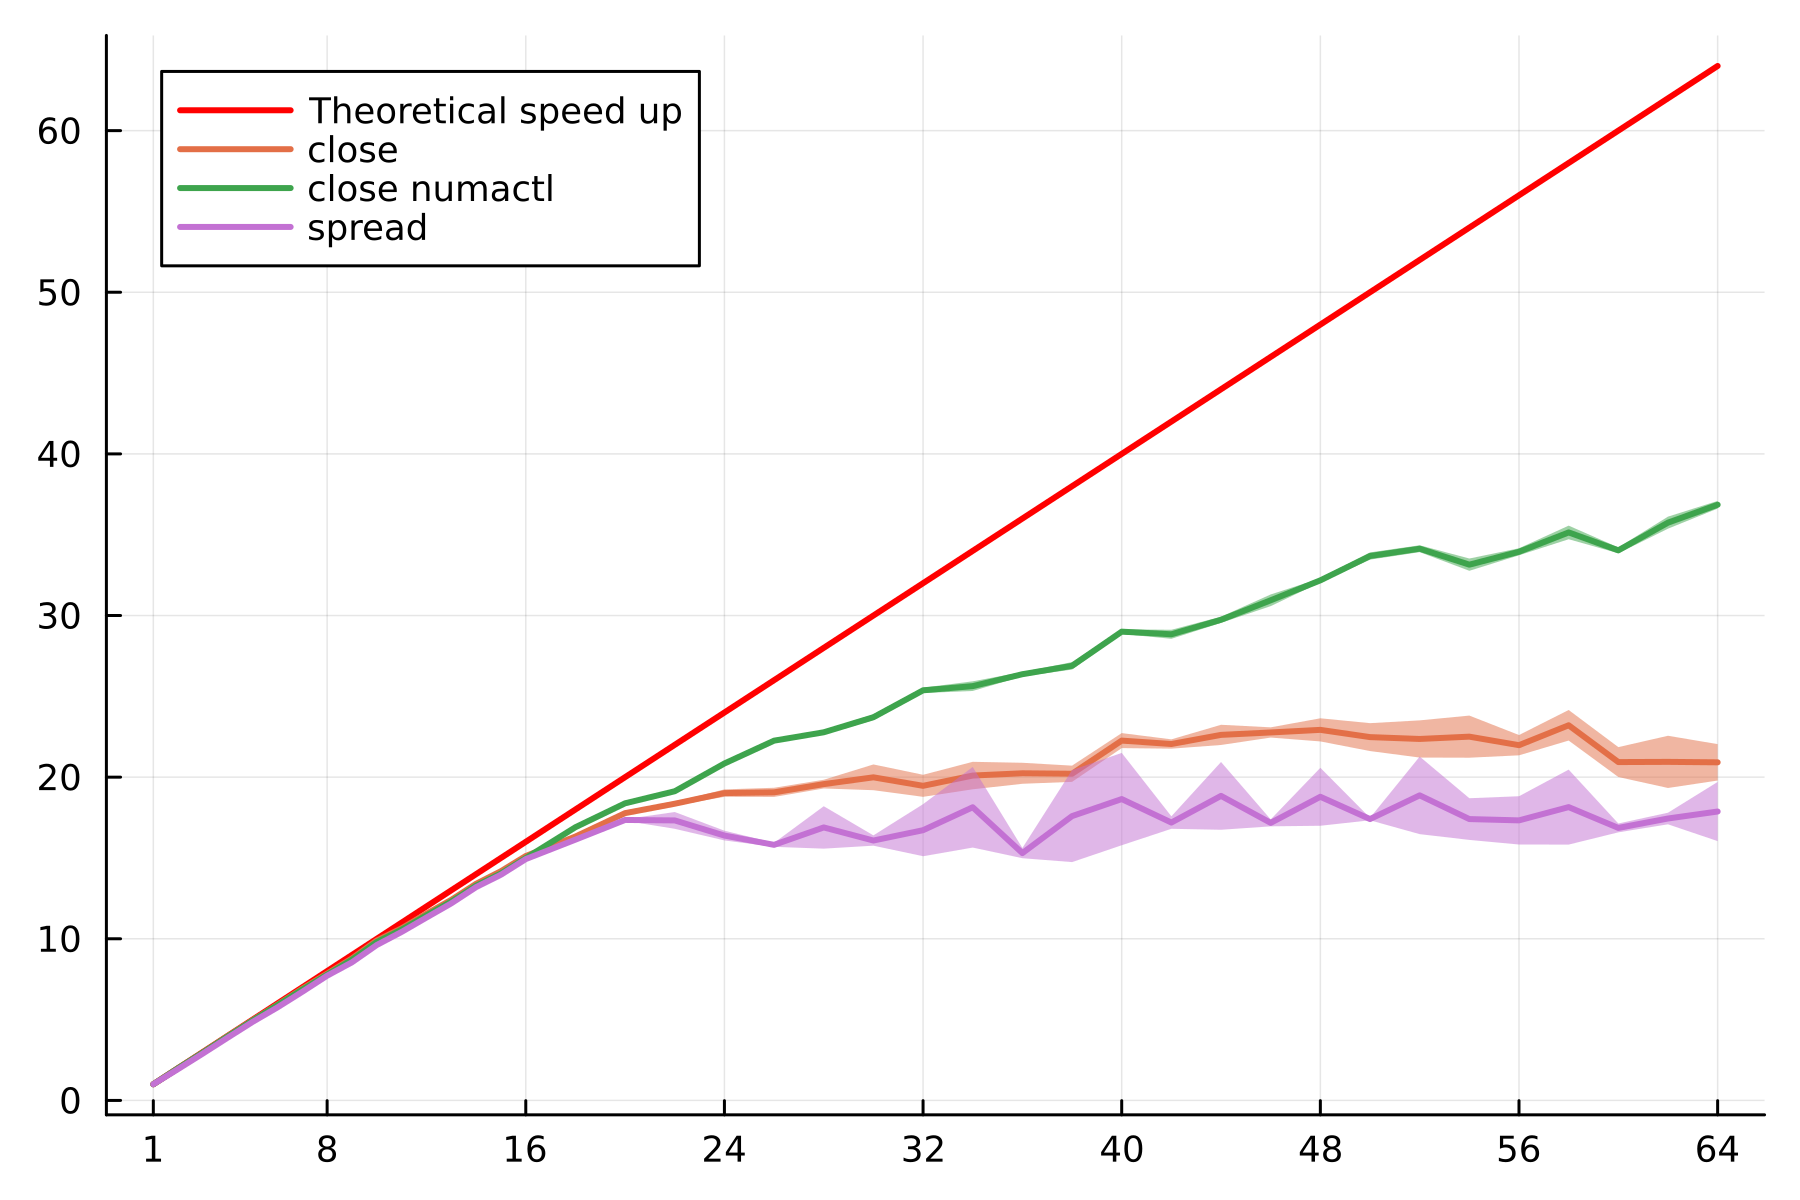
\includegraphics[width=\textwidth,height=3.64583in]{img/oblas_scalability_double_20000.png}

}

\caption{OpenBlas scalability, n=m=k=20000 - Double}

\end{figure}

\begin{figure}

{\centering 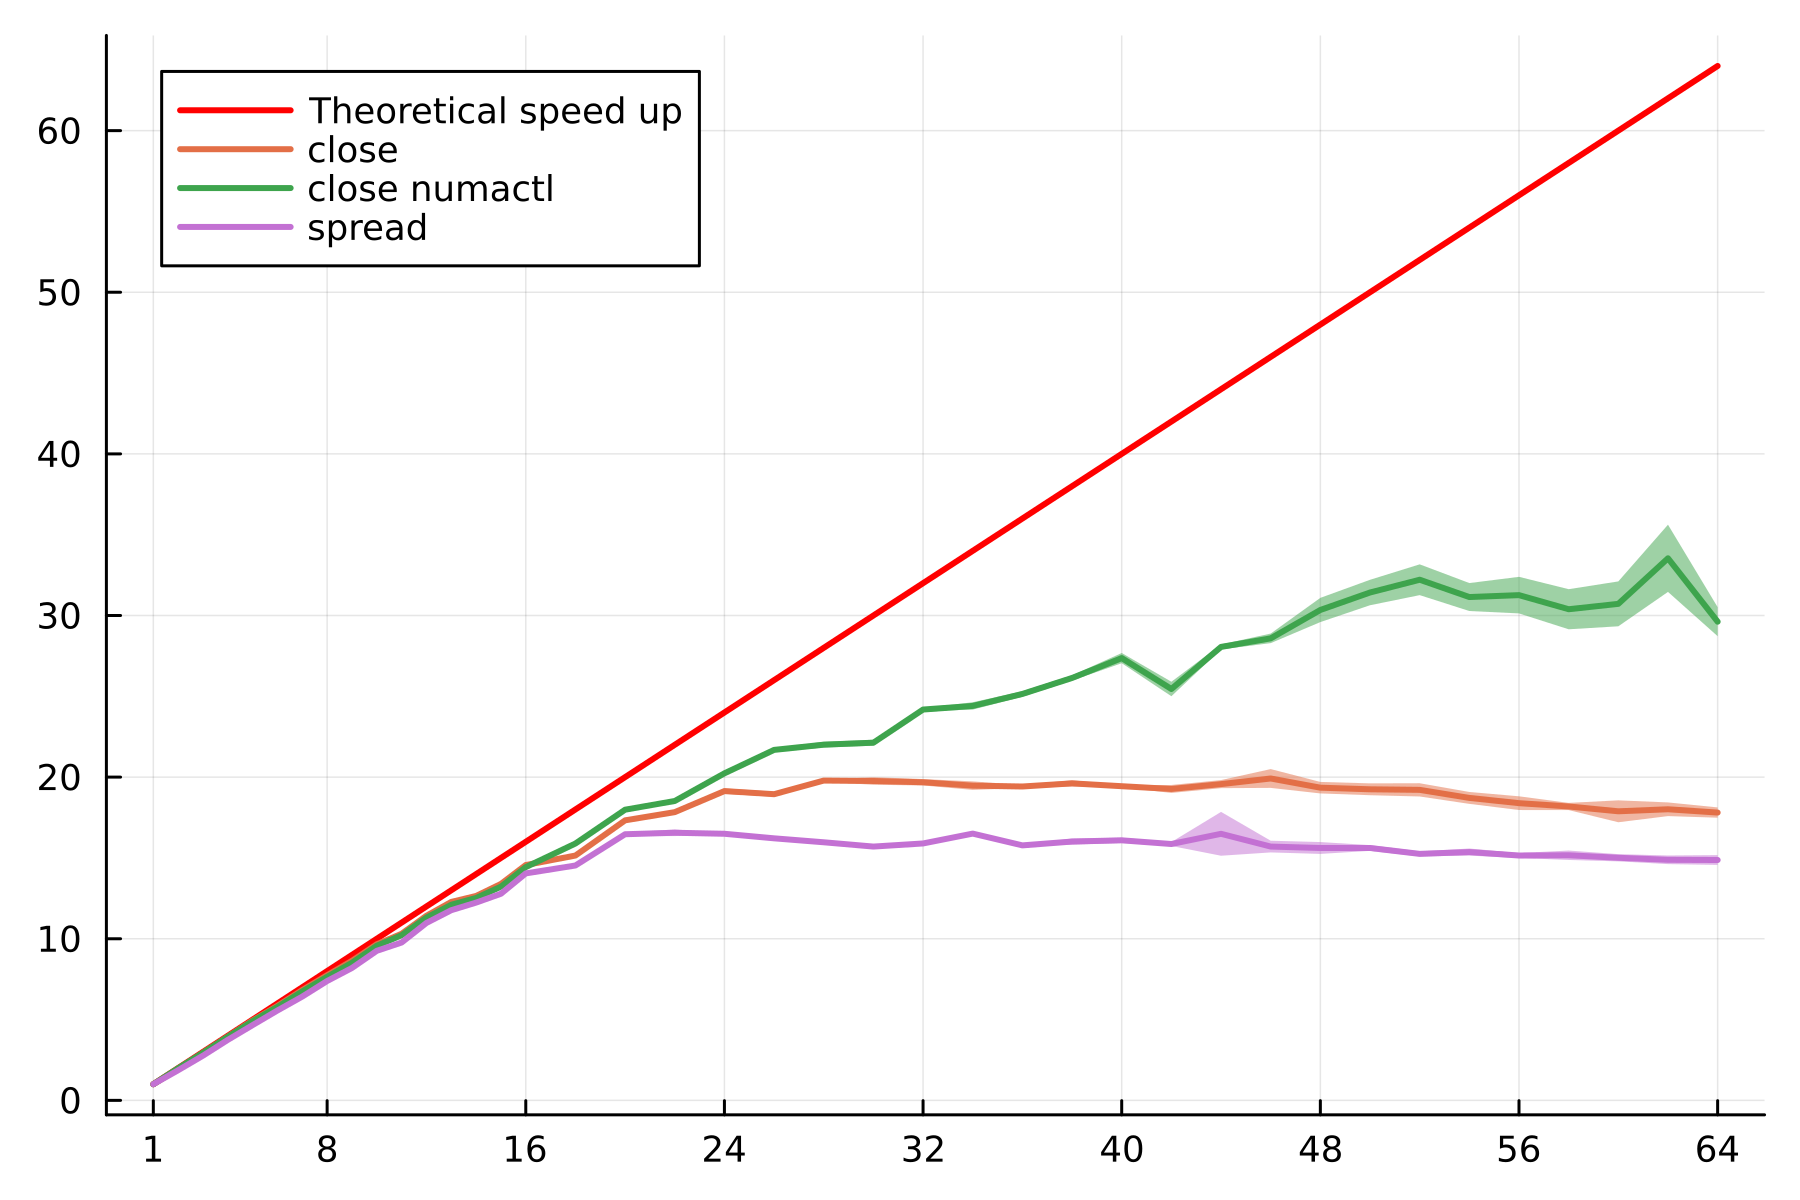
\includegraphics[width=\textwidth,height=3.64583in]{img/oblas_scalability_double_10000.png}

}

\caption{OpenBlas scalability, n=m=k=10000 - Double}

\end{figure}

\begin{figure}

{\centering 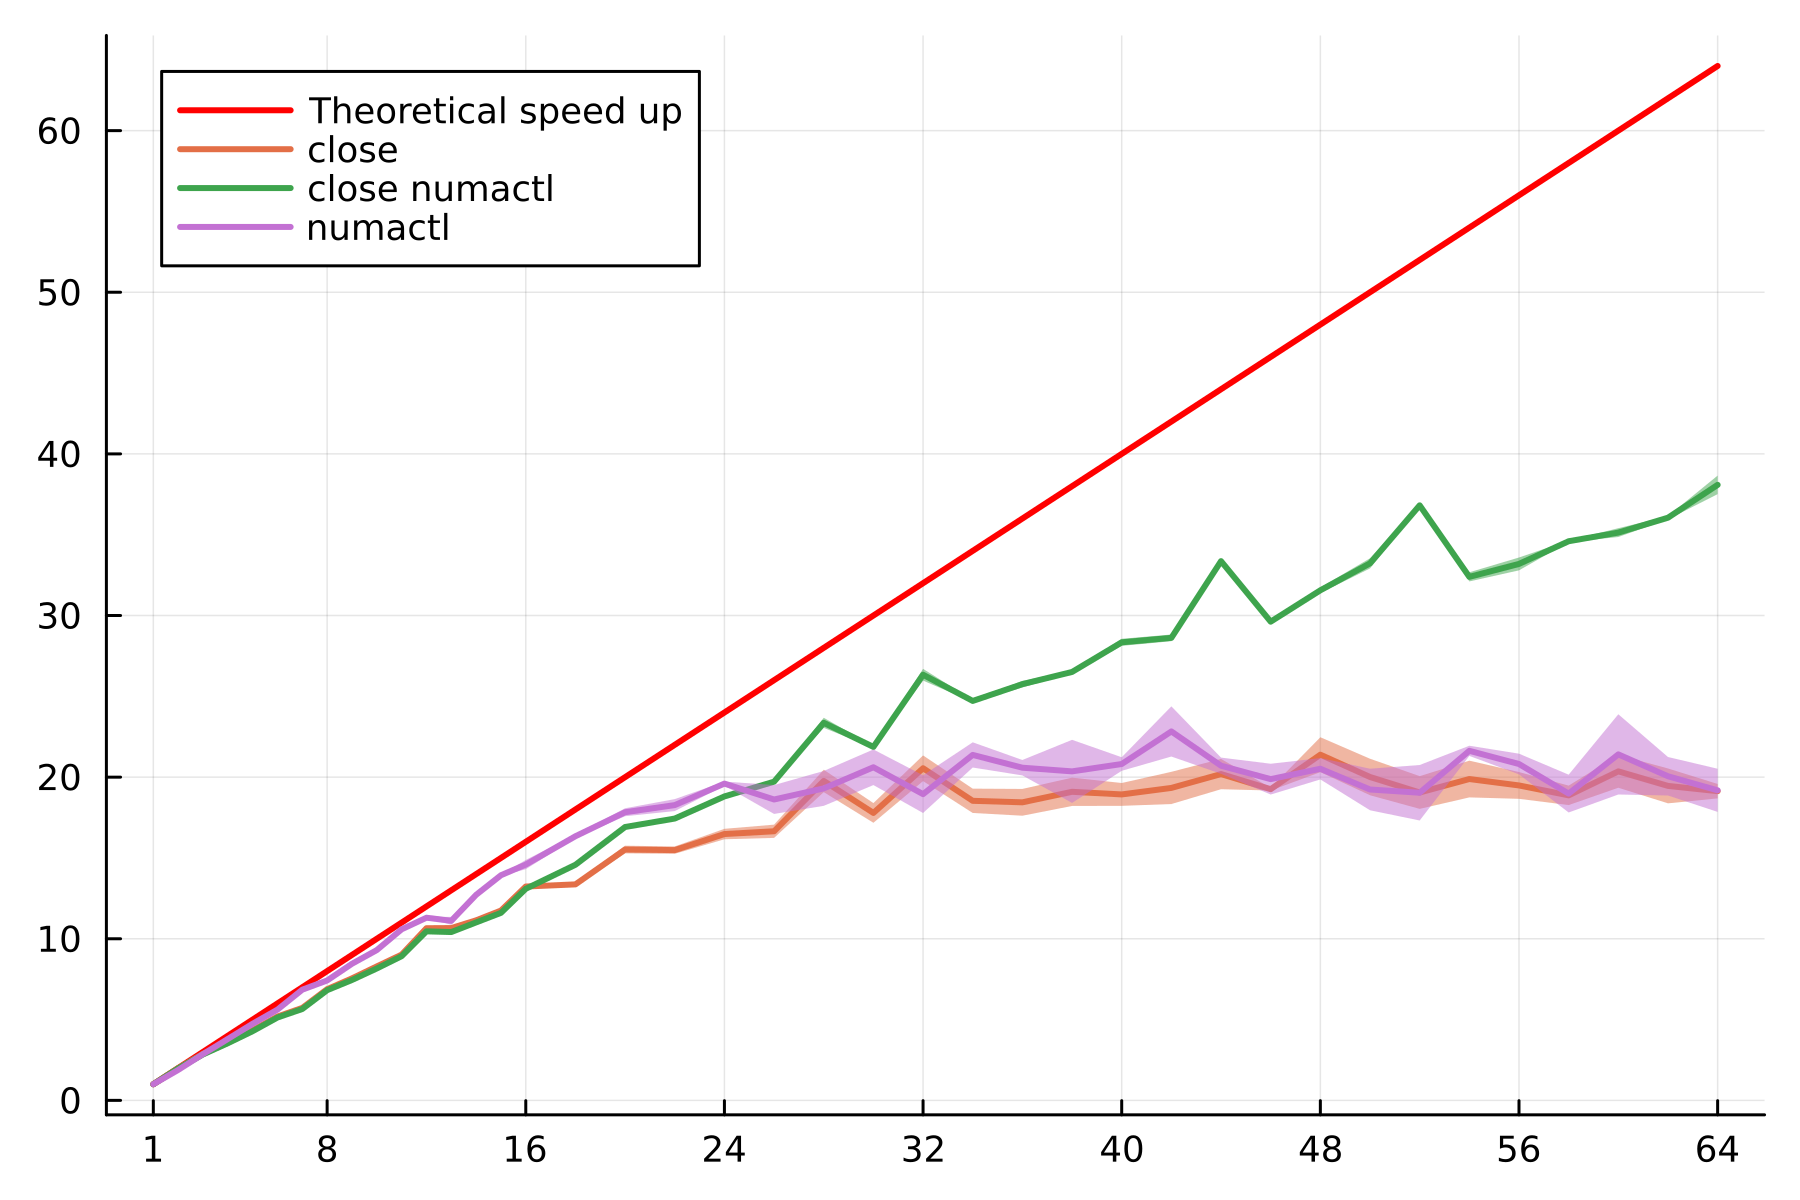
\includegraphics[width=\textwidth,height=3.64583in]{img/blis_scalability_double_20000.png}

}

\caption{Blis scalability, n=m=k=20000 - Double}

\end{figure}

\begin{figure}

{\centering 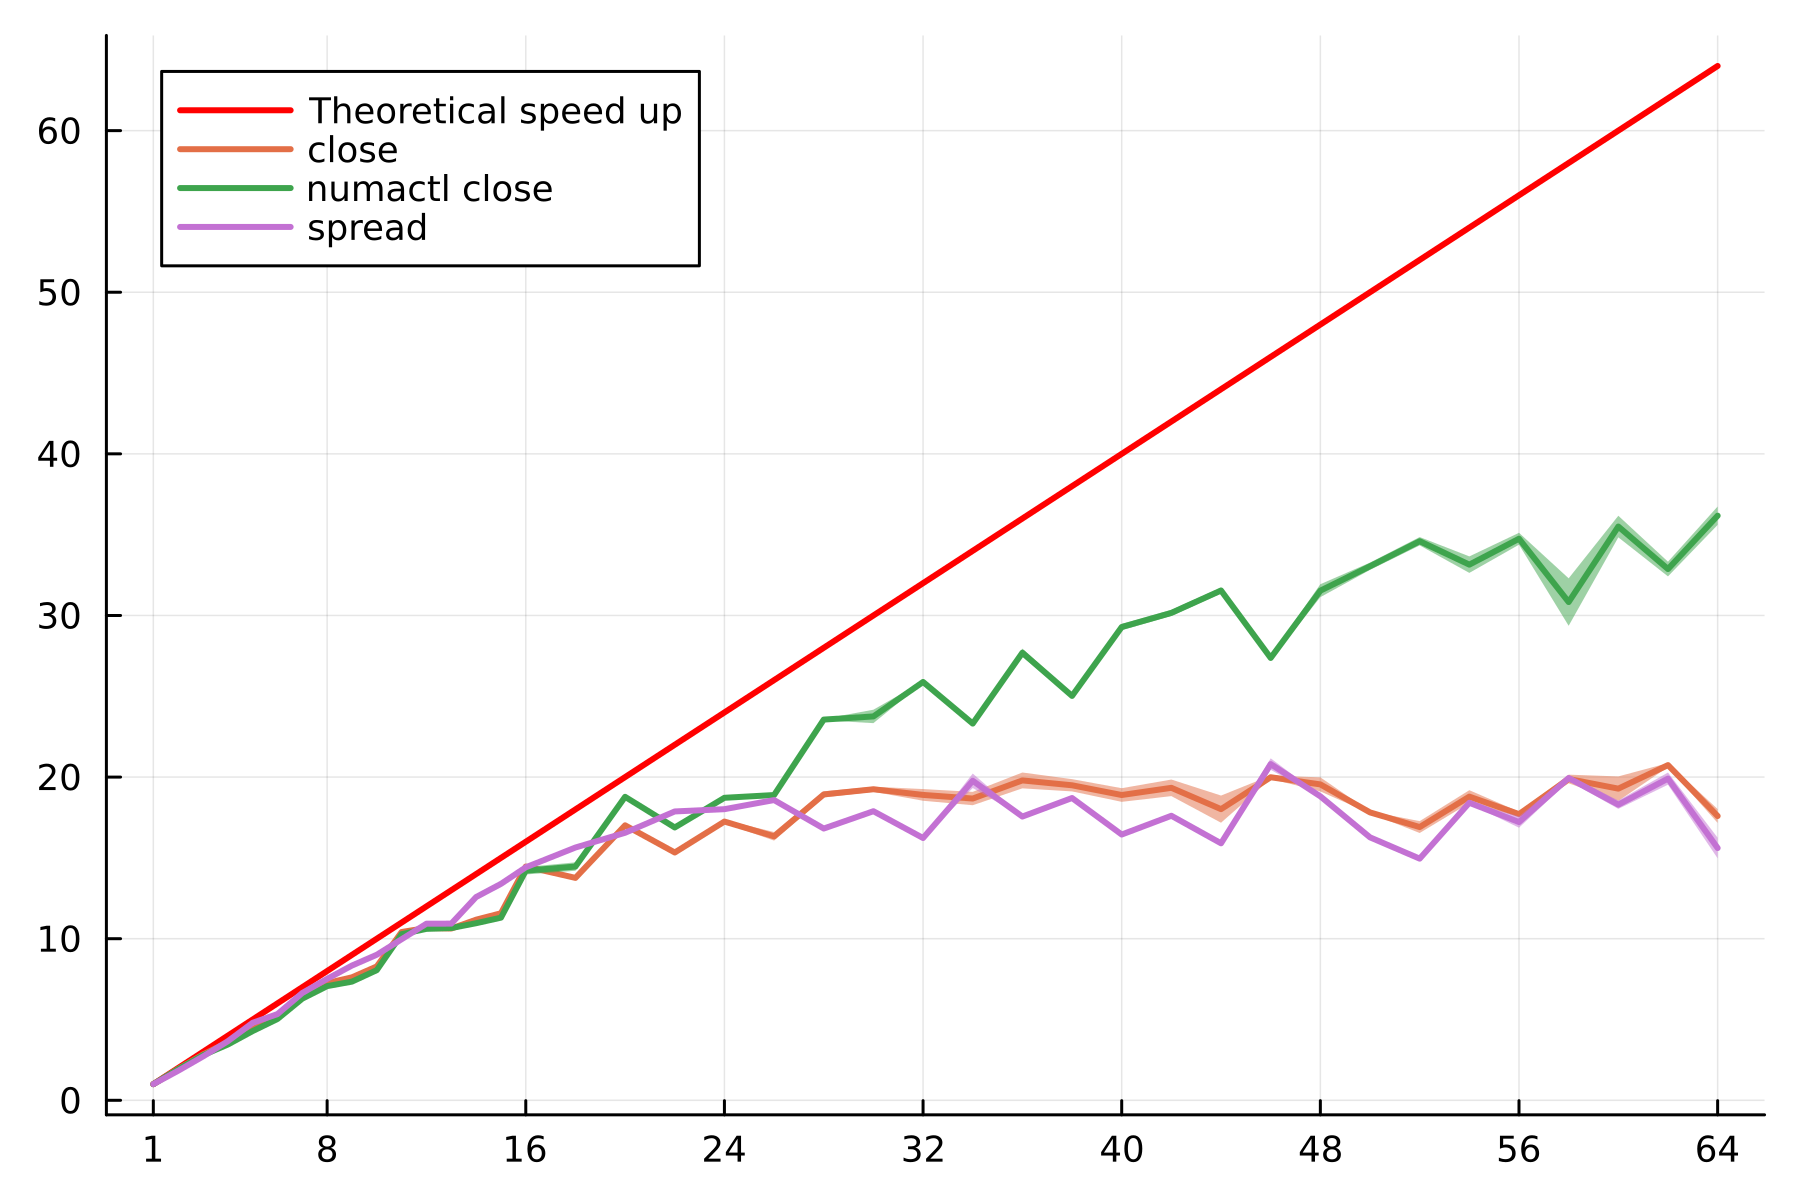
\includegraphics[width=\textwidth,height=3.64583in]{img/blis_scalability_double_10000.png}

}

\caption{Blis scalability, n=m=k=10000 - Double}

\end{figure}

\begin{figure}

{\centering 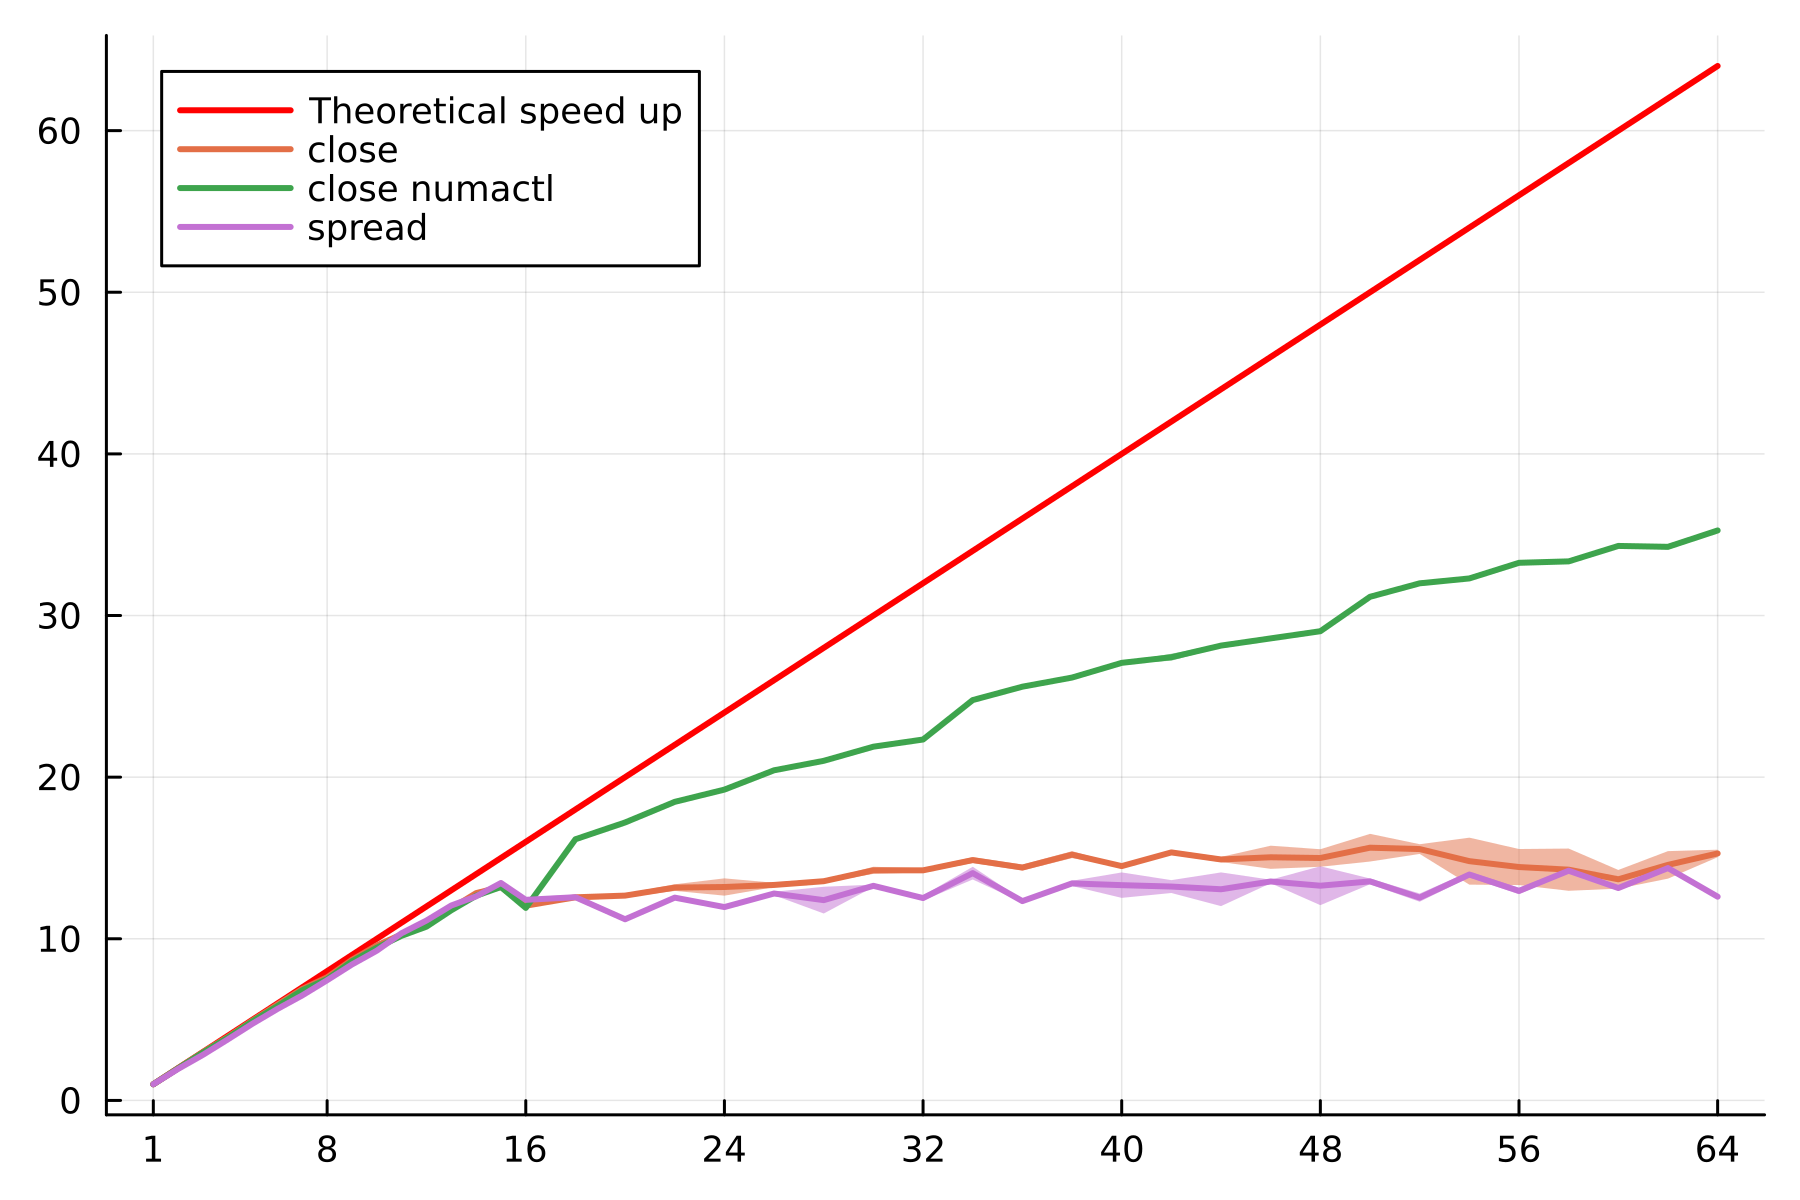
\includegraphics[width=\textwidth,height=3.64583in]{img/mkl_scalability_double_20000.png}

}

\caption{MKL scalability, n=m=k=20000 - Double}

\end{figure}

\begin{figure}

{\centering 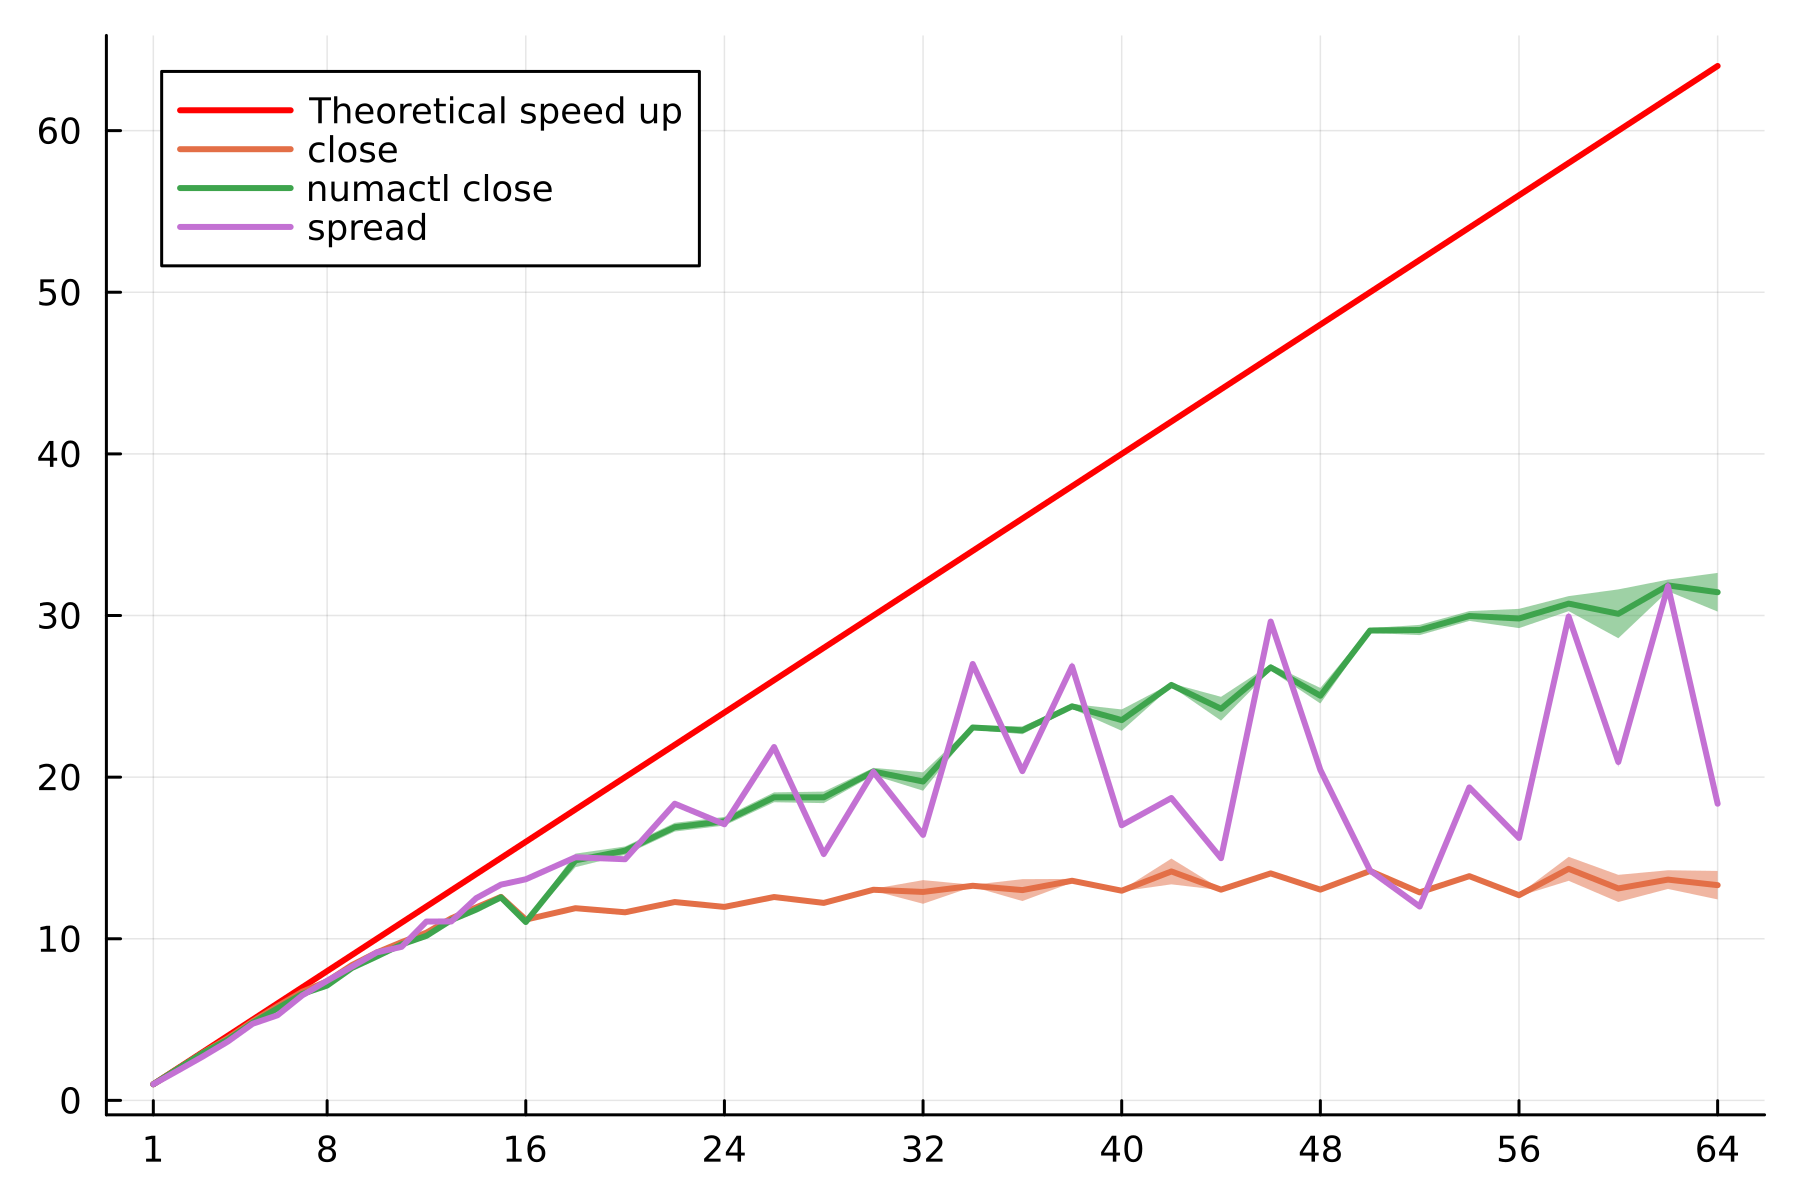
\includegraphics[width=\textwidth,height=3.64583in]{img/mkl_scalability_double_10000.png}

}

\caption{MKL scalability, n=m=k=10000 - Double}

\end{figure}



\end{document}
